%%%%%%%%%%%%%%%%%%%%%%%%%%%%%%%%%%%%%%%%%%%%%%%%%%%%%%%%%%%%
\documentclass[a4paper,english]{report}    % list options between brackets

\RequirePackage[dvips]{color}
\RequirePackage{setspace}
\RequirePackage{floatflt,epsfig}
\RequirePackage{float}
\RequirePackage{amsfonts}
\RequirePackage{amsmath}
\RequirePackage{alltt}
\RequirePackage[sectionbib]{chapterbib}
\RequirePackage{ae}
\RequirePackage{times}
\RequirePackage{fancyheadings}
\RequirePackage{multirow}

\usepackage{makeidx}  
\makeindex             

%%%%%%%%%%%%%%%%%%%%%%%%%%%%%%%%%%%%%%%%%%%%%%%%%%%%%%%%%%%%

\newcommand{\Sf}[1]{\textsf{#1}}
\newcommand{\Bf}[1]{{\sffamily\bfseries}}
\newcommand{\Bfm}[1]{\mbox{\boldmath{${#1}$}}}
\newcommand{\URL}[1]{\texttt{#1}}

% Some new commands...
\def\xwin{X Window System}
\def\xbr{Xbrowse}
\def\prag{\Tt{\#pragma}}

\newcommand{\inxgra}[2]{{\centerline{\includegraphics[width=#1]{#2}}}}
\newcommand{\inygra}[2]{{\centerline{\includegraphics[height=#1]{#2}}}}
\newcommand{\incgra}[2]{{\centerline{\includegraphics[height=#1]{#2}}}}

\providecommand{\ftn}{Fort\-ran~90}
\providecommand{\Idx}[1]{{#1}\index{#1}}

\newcommand{\ttbegin}{\begin{alltt}}
\newcommand{\ttend}{\end{alltt}}
\newcommand{\keno}{$\backslash$}
%%%%%%%%%%%%%%%% Definitions for Elmer Solver Manuals %%%%%%%%%%%%%%%%%

%\newcommand{\Vec}[1]{\mathify{\mathbf{#1}}}
%\newcommand{\Vec}[1]{\vec{#1}}
\newcommand{\Div}{\nabla\cdot}
\newcommand{\Curl}{\nabla\times}
\newcommand{\Grad}{\nabla}


\definecolor{SifCol}{rgb}{0.5,0.5,0.5}
%normal item, with text also (2 parameters + text)
\newcommand{\sifitem}[2]{\item[\tt{#1}]\hspace{1mm}{\color{SifCol}\hspace{1mm}\tt{#2}}\newline} 
%item with two fields but no text
\newcommand{\sifitemnt}[2]{\item[\tt{#1}]\hspace{1mm}{\color{SifCol}\hspace{1mm}\tt{#2}}} 
\newcommand{\sifbegin}{\begin{description}}
\newcommand{\sifend}{\end{description}}
\newcommand{\modinfo}[2]{{\bf{#1}}: {#2}\newline}

\newcommand{\Matr}[1]{\mbox{\boldmath{${#1}$}}}
\newcommand{\Der}[2]{\frac{\partial{#1}}{\partial{#2}}}
\newcommand{\Secder}[2]{\frac{\partial^2{#1}}{\partial{#2}^2}}
\newcommand{\Inv}[1] {\frac{1}{#1}}
%\DeclareMathOperator{\Div}{div}
%\DeclareMathOperator{\Grad}{grad}
%\DeclareMathOperator{\Curl}{curl}

% Use these to make the printable area bigger
% Also have the option 'ownsize' active in the documentclass
\setlength{\hoffset}{-15mm}
\setlength{\voffset}{-10mm}
\addtolength{\textwidth}{30mm}
\addtolength{\textheight}{20mm}
%\addtolength{\headwidth}{30mm}

% Make the headings fancier
\pagestyle{fancy}
\lhead[\normalfont\small\bf\thepage]{\normalfont\small\slshape\rightmark}
\rhead[\small\slshape\lefthead]{\normalfont\small\bf \thepage}
\setlength{\headrulewidth}{0.4pt}
%\renewcommand{\chaptermark}[1]{\markright{\bf \chaptername \ \thechapter.\ #1}{}}
\renewcommand{\chaptermark}[1]{\markright{\bf \thechapter.\ #1}{}}
\renewcommand{\sectionmark}[1]{}
\renewcommand{\subsectionmark}[1]{}
\cfoot{}


% This sets the Elmer version in the documentation
\newcommand{\elmerversion}{~5.4}



%%%%%%%%%%%%%%%%%%%%%%%%%%%%%%%%%%%%%%%%%%%%%%%%%%%%%%%%%%%%

\title{\Huge{\bf ElmerSolver Manual} \\ \mbox{} \\
\huge{\bf Still Under Construction!}}
\author{CSC, the Finnish IT Center for Science}
\date{\today}

%%%%%%%%%%%%%%%%%%%%%%%%%%%%%%%%%%%%%%%%%%%%%%%%%%%%%%%%%%%%

\begin{document}
\maketitle

\chapter*{Copyrights}

This document gives practical examples of the use of Elmer,
a finite element software for multiphysical problems.
The copyright if this document and Elmer software belong to
CSC -- IT Center for Science, Finland, 1995--2008. 

Elmer program is free software; you can redistribute it and/or
modify it under the terms of the GNU General Public License
as published by the Free Software Foundation; either version 2
of the License, or (at your option) any later version.

This program is distributed in the hope that it will be useful,
but WITHOUT ANY WARRANTY; without even the implied warranty of
MERCHANTABILITY or FITNESS FOR A PARTICULAR PURPOSE.  See the
GNU General Public License for more details.

CSC assumes no responsibility or liability on any errors or inaccuracies in 
Elmer program or documentation. Any kind of material damages or other indirect
consequences resulting from any Elmer part, documentation discrepancies and 
errors or non-anticipated program behavior are limited to the value of 
appropriate products purchased from CSC. 

This document is for informational use only. All information and specifications
given have been carefully prepared by the best efforts of CSC, and are believed
to be true and accurate as of time publishing. CSC reserves the right to 
modify Elmer and its documents without notice. \\  \mbox{} \\

\textbf{Additional software product copyrights included in Elmer}

Copyright, and License:

UMFPACK Version 4.3, Jan. 16, 2004. Copyright (c) 2004 by Timothy
A. Davis, University of Florida, davis@cise.ufl.edu. All Rights
Reserved. 


UMFPACK License: 

Your use or distribution of UMFPACK or any derivative code implies
that you agree to this License. 

      THIS MATERIAL IS PROVIDED AS IS, WITH ABSOLUTELY NO WARRANTY
      EXPRESSED OR IMPLIED. ANY USE IS AT YOUR OWN RISK. 

      Permission is hereby granted to use or copy this program,
      provided that the Copyright, this License, and the Availability
      of the original version is retained on all copies. User
      documentation of any code that uses UMFPACK or any modified
      version of UMFPACK code must cite the Copyright, this License,
      the Availability note, and "Used by permission." Permission to
      modify the code and to distribute modified code is granted,
      provided the Copyright, this License, and the Availability note
      are retained, and a notice that the code was modified is
      included. This software was developed with support from the
      National Science Foundation, and is provided to you free of
      charge. 


\chapter*{About ElmerGrid Manual}

The ElmerGrid Manual is part of the documentation of 
Elmer finite element software package.
ElmerGrid Manual gives instruction 
on the usage of ElmerGrid, the mesh generation and manipulation utility of Elmer.

The present ElmerGrid Manual
corresponds to software version \elmerversion{}.
The latest versions of Elmer software and its documentation
are available at the Elmer homepage at
\URL{http://www.csc.fi/elmer}. 




%%%%%%%%%%%%%%%%%%%%%%%%%%%%%%%%%%%%%%%%%%%%%%%%%%%%%%%%%%%%

\pagestyle{empty}
% Table of contents:
\setcounter{secnumdepth}{2}
\setcounter{tocdepth}{1}  
\tableofcontents

%%%%%%%%%%%%%%%%%%%%%%%%%%%%%%%%%%%%%%%%%%%%%%%%%%%%%%%%%%%%

\newpage
%\renewcommand{\chaptername}{Chapter}
%\pagenumbering{arabic}
\pagestyle{fancy}

%%%%%%%%%%%%%%%%%%%%%%%%%%%%%%%%%%%%%%%%%%%%%%%%%%%%%%%%%%%%


% input file
\graphicspath{{./}{input/}}
\chapter{Solver Input File}
\noindent
                                                                                                                 
\section{Introduction}

Solving partial differential equation (PDE) models with the solver of Elmer
requires that a precise description of the problem is given using 
the so-called solver input file\index{solver input file}, briefly referred to as the sif file. 
This file contains user-prepared input data which specify the location of mesh files and 
control the selection of physical models, material parameters, boundary conditions, 
initial conditions, stopping tolerances for iterative solvers, etc. 
In this chapter, the general structure of the file is described. We explain
how the input data is organized into different sections and describe the general keyword syntax 
which is used in these sections to define the values of various model parameters and to control
the solution procedures.

In the case of simple problem setups the solver input file may be written automatically by 
the preprocessor of Elmer software, so that knowing the solver input file format may be unnecessary.
Creating a more complicated setup, or using keywords introduced by the user, however, requires 
the knowledge of the file format and keyword syntax. 

In the following the general structure of the input file is first illustrated by using simple examples,
without trying to explain all possibilities in an exhaustive manner.
We then describe the keyword syntax in more detail, showing also how model parameters 
whose values depend on solution fields can be created. The later chapters of this manual, 
and Elmer Models Manual, which focuses on describing the PDE models Elmer can handle, provide more
detailed material on specific issues. Elmer Tutorial Manual also gives complete
examples of solver input files.

%Such dependencies can generally be created by means of
%tabular data,  MATC  functions, or Fortran  functions. MATC has the benefit of being an interpreted 
%language, making an additional compilation step with a compiler unnecessary.

                                                                                                                 
%The solver input (.sif) file describes the
%computational case for the solver.  The
%input file is used to give the solver
%the mesh directory,  material parameters, initial
%conditions, boundary conditions, etc.
%One  may add his/her own keywords to the file,
%which solvers may ask using special runtime routines.
%The different parameters given in input file may
%depend on solution fields, and may be given as constants, tabulated
%values,  MATC  functions, or Fortran  functions. MATC is an
%interpreted language, which doesn't need any
%additional compilation step, or a compiler.

\section{The sections of solver input file}

The material of the solver input file is organized into different sections.  
Each section is generally started with a row containing the name of the section, followed by a number of
keyword commands, and ended with a row containing the word {\tt End}. 
The names for starting new sections are\index{solver input file!section names}
\begin{itemize}
\item {\tt Header}
\item {\tt Simulation}
\item {\tt Constants}
\item {\tt Body n}
\item {\tt Material n}
\item {\tt Body Force n}
\item {\tt Equation n}
\item {\tt Solver n}
\item {\tt Boundary Condition n}
\item {\tt Initial Condition n}
\end{itemize}
Here {\tt n} associated with the section name represents an integer identifier needed for distinguishing between 
sections of the same type. A basic keyword command included in a section
is nothing more than a statement which sets the value of a keyword
with an equal sign. 

In the following we describe how the sections are basically arranged without 
trying to explain all possibilities in an exhaustive manner. 
The later chapters of this manual and Elmer Models Manual provide more
detailed material on specific issues. Elmer Tutorial Manual also gives complete
examples of solver input files. 

\paragraph{Header section.}
The location of mesh files is usually given in the header section. Often this is also
the only declaration given in the header section. If the Elmer mesh files (see Appendix A) are located in the 
directory ./1d, the header section may simply be 
% A sample input file header might be 
\ttbegin
Header
  Mesh DB "." "1d"
End
\ttend
Note that separate equations can nevertheless be discretized using different meshes if the location of mesh files is given 
in the solver section described below. 
%Other commands that may be given in the header section are 

\paragraph{Simulation section.}
The simulation section is used for giving general information that is not specific
to a particular PDE model involved in the simulation. This information describes the coordinate system used,
indicates whether the problem is stationary or evolutionary, defines the file names for outputting, etc.
%The simulation
%section contains several fields that concern the case as a whole:
Without trying to describe many possibilities and the details of commands, 
we only give the following simple example:  
\ttbegin
Simulation
  Coordinate System = "Cartesian 1D"
  Coordinate Mapping(3) = 1 2 3
  Simulation Type = Steady State
  Steady State Max Iterations = 1
  Output Intervals(1) = 1
  Post File = "1dheat.ep"
  Output File = "1dheat.dat"
End
\ttend



\paragraph{Constants section.}
The constants section is used for defining certain physical constants. 
For example the gravity vector and the Stefan-Boltzmann constant may be defined using the commands 
\ttbegin
Constants
  Gravity(4) = 0 -1 0 9.82
  Stefan Boltzmann = 5.67e-08
End
\ttend
If the constants are not actually 
needed in the simulation, this section can also be left empty. 

\paragraph{Body, material, body force and initial condition sections.} 
The Elmer mesh files contain information on how the computational region
is divided into parts referred to as bodies. A body section associates
each body with an equation set, material properties, body forces, and initial conditions by 
referring to definitions given in a specified equation section, material section, body force section, and
initial condition section. To manage to do this, the different sections of the same type are distinguished
by integer identifiers that are parts of the section names. Note that the integer in the body section name 
is an identifier for the body itself. 

For example, one may define 
\ttbegin
Body 1
  Material = 1
  Body Force = 1
  Equation = 1
  Initial Condition = 2
End
\ttend
Material properties, body forces, an equation set, and initial conditions 
are then defined in the material section 
\ttbegin
Material 1
  ...
End
\ttend
the body force section
\ttbegin
Body Force 1
  ...
End
\ttend
the equation section
\ttbegin
Equation 1
  ...
End
\ttend
and the initial condition section
\ttbegin
 Initial Condition 2
  ...
End
\ttend
What material properties and body forces need to be specified depends on the mathematical models 
involved in the simulation, and the initial condition section used for giving initial values is only relevant
in the solution of evolutionary problems. We here omit the discussion of these very model-dependent 
issues; after reading this introductory chapter the reader should be able to understand
the related documentation given in Elmer Models Manual, which focuses on describing the different mathematical models,
while the contents of equation section will be described next.

%The computational domain might consist of several different subdomains or
%'bodies', for each body the equation definition section, initial condition
%section, body force section and material definition section numbers are
%given. These sections are described later.
%\ttbegin
%Body
%  Equation = 1
%  Material = 1
%  Body Force = 1
%End
%\ttend

%The body force definition is used to give the volume forces, if any,
%for the equation solvers. Here a source term for the Poisson equation
%is given as constant 1:

%\ttbegin
%Body Force 1
%  Source = Real 1
%End
%\ttend

\paragraph{Equation and solver sections.}
Equation section provides us a way to associate each body with a set of equation solvers. 
That is, if the set defined consists of more than one equation solver, several physical phenomena 
may be considered to occur simultaneously over the same region of space.
Individual equation solvers are actually defined in solver sections, the contents of an equation section
being basically a list of integer identifiers for finding the solver sections that define the solvers.
%The equation section defines the set of equation solvers for a subdomain
%of the whole computational  domain to be activated.  Note that previously
%we attached the equation definition to a body definition. This time only
%one equation solver is activated.
The keyword commands given in the solver sections then control the selection of physical models, 
linearization procedures of nonlinear models, 
the selection of solution methods for resulting linear equations, convergence tolerances, etc.  

For example, if only two solvers are needed, one may simply define a list of two solver identifiers 
\ttbegin
Equation 1
  Active Solvers(2) = 1 2
End
\ttend
%The solver sections are used to define the equations solver and all the
%solver dependent parameters, such as linear system solver options, and
%the file name and name of the solver procedure, the name of the solver
%variable, etc.
Then the solver definitions are read from the solver sections 
\ttbegin
Solver 1
  ...
End
\ttend
and 
\ttbegin
Solver 2
  ...
End
\ttend
Finally, we give an example of solver definitions, without trying to explain the commands at this point:
\ttbegin
Solver 1
 Equation = "Poisson"
 Variable = "Potential"
 Variable DOFs = 1
 Procedure = "Poisson" "PoissonSolver"
 Linear System Solver = "Direct"
 Steady State Convergence Tolerance = 1e-06
End
\ttend

\paragraph{Boundary condition section.}Boundary condition sections define the boundary conditions for the different
equations. The Elmer mesh files contain information on how the boundaries of the bodies are divided
into parts distinguished by their own boundary numbers. The keyword {\tt Target Boundaries} is used to list 
the boundary numbers that form the domain for imposing the boundary condition. 
%The boundary condition is mapped to boundaries of the mesh by
%giving the keyword Target Boundaries. Below the meaning is that Boundary
%Condition 1 is attached to boundaries 1, and 2:
For example the declaration 
\ttbegin
Boundary  Condition 1
  Target Boundaries(2) = 1 2
  ...
End
\ttend
means that the boundary condition definitions that follow concern the two parts having the boundary numbers 1 and 2.

\paragraph{}
We finally note that some commands, such as comments started with the symbol ! and MATC expressions described below, 
may also be placed outside section definitions. An exception of this type is also the command
\ttbegin
Check Keywords "Warn"
\ttend
usually placed in the beginning of the input file. When this command is given, the solver 
outputs warning messages if the input file contains keywords that are not listed in the file
of known keywords. If new keywords are introduced, misleading warning messages can be avoided
by adding the new keywords to the keyword file {\tt SOLVER.KEYWORDS}, located in the directory
of the shared library files of ElmerSolver. 
 
 


\section{Keyword syntax}\index{keyword syntax}
As already illustrated,
a basic keyword command used in the solver input file
is a statement which sets the value of a solution parameter with the equal sign.
Such a command in its full form also contains the data type declaration; for example
\ttbegin
Density = Real 1000.0
\ttend
Valid data types generally are
\begin{itemize}
\item {\tt Real}
\item {\tt Integer}
\item {\tt Logical}
\item {\tt String}
\item {\tt File}
\end{itemize}
If the keyword is listed in the keyword file {\tt SOLVER.KEYWORDS}, the data type declaration
may be omitted. Therefore, in the case of our example, we may also define
\ttbegin
Density = 1000.0
\ttend

The value of a keyword may also be an array of elements of specified data type, 
with the array size definition associated with the keyword. We recall our previous examples
of the equation and boundary condition sections, where we defined two lists of integers
using the commands
\ttbegin
Active Solvers(2) = 1 2
\ttend
and
\ttbegin
Target Boundaries(2) = 1 2
\ttend
Two-dimensional arrays are also possible and may be defined as
\ttbegin
My Parameter Array(3,3) = Real 1 2 3 \keno
                               4 5 6 \keno
                               7 8 9 

\ttend
%A keyword may be defined to be a array insted of a scalar
%value, the array may be defined by giving the size of the array as in

%If the keyword is not known to the Elmer Solver the type of the
%value  must also be given
%
%\ttbegin
%My Parameter = Real 1000
%\ttend


\paragraph{Defining parameters depending on field variables.}
Most solver parameters may depend on time, or on the field variables defined in the current simulation run. 
Such dependencies can generally be created by means of
tabular data,  \Idx{MATC}  functions, or Fortran  functions. MATC has the benefit of being an interpreted 
language, making an additional compilation step with a compiler unnecessary.

Simple interpolating functions can be created by means of tabular data. The following example
defines the parameter {\tt Density} the value of which depends on the variable 
{\tt Temperature}:
\ttbegin
Density = Variable Temperature
  Real
    0    900
    273 1000
    300 1020
    400 1000
End
\ttend
This means that the value of {\tt Density} is 900 when {\tt Temperature} is 0, and
the following lines are interpreted similarly. Elmer then uses linear interpolation
to approximate the parameter for argument values not given in the table.
%linearily interpolated between 0-273 between values 900 and 1000, etc.
If the value of the independent variable is outside the data set,
the first or the last interpolating function which can be created from the
tabulated values is used to extrapolate the value of the parameter. 

If the field variable has several independent components, such as the components of
displacement vector, the independent components may be used as arguments in 
a function definition.  
%The components of the array valued variables (defined for example in solver
%section) are given a name with the component number attached, i.e. 
For example, if a three-component field variable is defined in a solver section
using the commands
\ttbegin
Variable = "Displ"
Variable DOFs = 3
\ttend
then the solver of Elmer knows, in addition to the three-component vector {\tt Displ}, 
three scalar fields {\tt Displ 1}, {\tt Displ 2} and {\tt Displ 3}. 
These scalar fields may be used as independent variables in parameter definitions,
and used in the definitions of initial and boundary conditions, etc.

More complicated functions can be defined using MATC language.\index{MATC} Here the basic usage 
of MATC in connection with the solver input file is illustrated; 
for an additional documentation, see a separate manual for MATC. For example,
one may define
\ttbegin
Density = Variable Temperature
  MATC "1000*(1-1.0e-4*(tx-273))"
\ttend
This means that the parameter {\tt Density} depends on the value of {\tt Temperature} as
\begin{equation}
  \rho =  \rho_0(1-\beta(T-T_0)),
\end{equation}
with $\rho_0=1000, \beta=10^{-4}$ and $T_0=273$. Note that
the value of the independent variable is known as {\tt tx} in the MATC expression.
%Similarly, the variable {\tt st} is the current steady state iteration
%number or simulation time, if a steady, coupled problem or a transient problem, respectively,
%is solved.

If the independent variable has more than one component, the variable {\tt tx}
will contain all the components in values {\tt tx(0)},{\tt tx(1)},...,{\tt tx(n-1)}, where 
{\tt n} is the number of the components of the independent variable. 
A MATC expression may also take several scalar arguments; one may define, for example,
\ttbegin
My Parameter = Variable Time, Displ 1
  Real MATC "..."
\ttend
The values of the scalar fields {\tt Time} and {\tt Displ 1} 
can then be referred in the associated MATC expression by the names {\tt tx(0)} and {\tt tx(1)}, respectively.

In addition to using MATC functions, Fortran 90 functions may also be used to create parameter 
definitions, etc. In the same manner as MATC functions are used, we may define
\ttbegin
Density  = Variable Temperature
  Procedure "filename" "proc"
\ttend
In this case the file "filename" should contain a shareable .so (Unix) or .dll
(Windows) code for the user function whose name is "proc".  The call interface
for the Fortran function is as follows
\ttbegin
FUNCTION proc( Model, n, T ) RESULT(dens)
  USE DefUtils)
  IMPLICIT None
  TYPE(Model_t) :: Model
  INTEGER :: n
  REAL(KIND=dp) :: T, dens

  dens = 1000*(1-1.0d-4(T-273.0d0))
END FUNCTION proc
\ttend
The Model structure contains pointers to all information about the model, and may be
used to obtain field variable values, node coordinates, etc. The argument n is
the index of the node to be processed, and T is the value of the independent variable
at the node. The function should finally return the value of the dependent
variable. 

The independent variable can also be composed of
several independent components. We may thus define
\ttbegin
Density = Variable Coordinate
  Procedure "filename" "proc"
\ttend
Now the argument T in the Fortran function interface should be a real array of three values, 
which give the x,y and z coordinates of the current node. 

%A keyword may be defined to be a array insted of a scalar
%value, the array may be defined by giving the size of the array as in
%
%\ttbegin
%Active Solver(2) = 1 2
%Target Boundaries(3) = 2 4 5
%My Parameter Array(3,3) = Real 1 2 3 \keno
%                               4 5 6 \keno
%                               7 8 9 
%
%\ttend


\paragraph{Parameterized keyword commands.}\index{MATC!parameterized keyword commands}
The solver input file also offers possibilities
for creating parameterized commands that utilize MATC. In the solver input file an expression 
following the symbol \$ is generally interpreted to be in MATC language. If the solver input file
contains the lines
\ttbegin
\$solvertype = "Iterative"
\$tol = 1.0e-6
\ttend
then one may define, e.g.,
\ttbegin
Solver 1
  ...
  Linear System Solver = \$solvertype
  Linear System Convergence Tolerance = \$tol
  ...
End

Solver 2
  ...
  Linear System Solver = \$solvertype
  Linear System Convergence Tolerance = \$100*tol
  ...
End
\ttend







\bibliography{elmerbib}
\bibliographystyle{plain}


% fem utilities
\graphicspath{{./}{fem/}}
\chapter{Finite Element Utilities}
\noindent

\section{Introduction}

This section decribes Elmer Solver utilities related directly to Finite Element Method (FEM).
Finite element method is a common procedure to solve differential and integral equations numerically.


\section{Theory}


\section{Higher-order finite elements}

\subsection{Theory}

Higher-order finite elements are elements for which the degree of basis functions is higher than $1$. They differ from usual Lagrange -type elements in a sense that in addition to nodal basis functions there exists basis functions, which are associated with edges, faces and interiors of elements.

\begin{itemize}
\item \textbf{Size modes} get their values along some edge of element. They vanish towards other edges and all nodal points of element. Side modes are defined for all 2d and 3d elements. 
\item \textbf{Face modes} get their values along some face of element. They vanish towards other faces and all edges and nodal points of element. Face modes are only defined for 3d elements. 
\item \textbf{Internal modes} get their values inside element and vanish towards elements faces, edges and nodal points. They are defined for all 1d, 2d and 3d elements. 
\end{itemize}

Higher-order elements are usually also called $p$ -elements. Properties for good $p$-elements include computational efficiency, at least partial orthogonality and hierarchy of basis functions. With hierarchy we mean that if basis for some element of some given degree $p$ is $\mathcal{B}^p$ for $p+1$ it holds that $\mathcal{B}^p \subset \mathcal{B}^{p+1}$. Orthogonal properties of basis functions ensure, that condition number of the global stiffness matrix does not increase as dramatically as for nodal (Lagrange) elements of higher order. This ensures good numerical stability. Some good references to higher-order finite elements in literature are \cite{SzaboBabu} by Szabo and Babuska and \cite{Solin} by Solin et al. 

The usual element interpolant, now denoted as $u_{h,p}$, is for $p$ elements the sum of nodal, edge, face and bubble interpolants

\begin{equation}
 u_{h,p}=u_{h,p}^v+u_{h,p}^e+u_{h,p}^f+u_{h,p}^b
\end{equation}

\noindent where $u_{h,p}^v$ is nodal interpolant as defined before and $u_{h,p}^e$ edge, $u_{h,p}^f$ face and $u_{h,p}^b$ bubble interpolants. Let $n_e$ be the number of edges and $n_f$ number of faces in an element. Edge and face interpolants are defined as

\begin{eqnarray*}
u_{h,p}^e &=& \sum_{i=1}^{n_e} u_{h,p}^{e_i} \\
u_{h,p}^f &=& \sum_{i=1}^{n_f} u_{h,p}^{f_i}
\end{eqnarray*} 

Contribution of one $p$ -element to global system is equivalent to that of $h$-element. Naturally for higher-order elements the number of local stiffness matrix elements to contribute to global system is greater, because of the larger number of basis functions.  

Generally using $p$ -elements yields a better approximation than using normal linear elements. In fact, convergence for $p$ elements is exponential when there are no singularities inside or on the boundary of the solution domain. When there are singular points inside the domain convergence is algebraic. If singular point is a nodal point convergence is twice that of $h$-method, otherwise it is equal to the $h$-method.

\subsection{Higher-order elements in Elmer}

Elements implemented in Elmer follow the ones presented in \cite{SzaboBabu}. Now let us define some orthogonal polynomials based on Legendre polynomials $P_i(x), i\geq 0$. So called lobatto shape functions $\phi_k$ are defined as 

\begin{equation}
\phi_k(\xi)=\sqrt{\frac{1}{2(2k-1)}}(P_{k}(\xi)-P_{k-2}(\xi)),\
k=2,3,\ldots 
\end{equation}

\noindent where $P_k$ are Legendre polynomials. Function $\phi$ has two of its roots at $\pm 1$, so now define another function, $\varphi_i$ as

\begin{equation}
\varphi_k(\xi)=\frac{4\phi_k(\xi)}{1-\xi^2},\ k=2,\ldots,p
\end{equation}

\noindent Functions $\phi_i$ and $\varphi_i$ are used to define higher order elements. Different element shapes and their their basis functions are defined in appendix \ref{app:pbasis}. Pyramidal element used in Elmer is based loosely to Devloos representation in \cite{Devloo}. 

In Elmer elements with varying polynomial degree $p$ may be used in the same mesh. It is also possible to combine elements of different types in the same mesh, as defined basis functions for edges and faces for different element types are compatible with one another. Pyramidal and wedge higher-order elements to connect tetrahedral and brick elements are also supported. To achieve best possible converge the use of pyramidal elements in a mesh should be kept to a minimum. Global continuity of higher order finite element space used is enforced by the solver, when method \texttt{ElementInfo} is used for obtaining basis functions values for elements.  

To combine elements of varying degree in mesh maximum rule is used. Thus if two or more elements share an edge and have differing polynomial degrees, maximum of edge's degrees is choosed as degree of global edge. 

To declare polynomial degree greater than one to an element, element definition in \texttt{mesh.elements} -file needs to be changed. For $p$ -elements, element definition syntax is 

\[
T_e[\mbox{p}p_e]
\]

\noindent where $T_e=\{202,303,404,504,605,706,808\}$ is the element type and $p_e\geq 1$ polynomial degree of element. Setting $p_e=0$ equals using normal linear basis defined in Elmer. For example, a triangle with polymial degree $4$ could be defined in mesh.elements file as follows

\[
303\mbox{p}4
\]

The actual number of degrees of freedom for edges, faces or bubbles of element types is defined by element polynomial degree $p$. Each degree of freedom in element is associated with some basis function. The following table gives the number of degrees of freedom for elements used in Elmer.  

\begin{table}[H]
\begin{tabular}{|l|c|c|c|c|}
\hline
Element & Nodes & Edges & Faces & Bubbles \\
\hline \hline
Line & $2$ & - & - & $p-1$ \\
\hline
Quadrilateral & $4$ & $4(p-1)$ & - & $\frac{(p-2)(p-3)}{2}$ \\
\hline
Triangle & $3$ & $3(p-1)$ & - & $\frac{(p-1)(p-2)}{2}$ \\
\hline
Brick & $8$ & $12(p-1)$ & $ 3(p-2)(p-3)$ &
$\frac{(p-3)(p-4)(p-5)}{6}$ \\
\hline
Tetrahedron & $4$ & $6(p-1)$ & $2(p-1)(p-2)$ &
$\frac{(p-1)(p-2)(p-3)}{6}$ \\
\hline
Wedge & $6$ & $9(p-1)$ & - & $\frac{(p-2)(p-3)(p-4)}{6}$ \\
(quad. face) & - & - & $\frac{3(p-2)(p-3)}{2}$ & - \\
(triang. face) & - & - & $(p-1)(p-2)$ & - \\
\hline
Pyramidi & $5$ & $8(p-1)$ & -  &  $\frac{(p-1)(p-2)(p-3)}{6}$ \\
(quad. face) & - & - & $\frac{(p-2)(p-3)}{2}$ & - \\
(triang. face) & - & - & $2(p-1)(p-2)$ & - \\
\hline
\end{tabular}
\end{table} 

It is worth noting, however, that used Solver (HeatSolve, StressSolve, etc.) used must be modified to support elements of higher degree. Usually this only consists of making local stiffness matrix and force vector larger. 

A $p$-element passed to Elmer gaussian point generator \texttt{GaussPoints} defined in module \texttt{Integration} returns enough integration points to integrate worst case product of two element basis functions. Here worst case is integration over two basis functions for which $p_m=\max\{p_e,p_f,p_b\}$. As gaussian quadrature is accurate to degree $p=2n-1$, where $n$ is the number of points used, number of points for each element is calculated from 

\begin{equation}
n=\frac{2p_m+1}{2}
\end{equation} 

\noindent and rounded up to nearest integer. To get the final number of points for multiple integrals, $n$ is raised to the power of element dimension. If integral includes a non-constant factor, i.e $\int_K \alpha \phi_i\phi_j$ where $\alpha$ is a function of degree $k$, numerical integration is not accurate and number of integration points needs to be set manually. Now minimum number of gaussian points to integrate element accurately becomes

\begin{equation}
n=\frac{\min{\{2p_m+k,3p_m\}}+1}{2}
\end{equation}

\noindent which may again be rounded up to nearest integer and raised to power of element dimension to get the actual number of integration points. 

\subsubsection{Boundary conditions}

Boundary elements (elements, which lie on a boundary of a computational domain) obey the parity of their parent element. Basis for elements on boundary is defined so that it represents a projection from high to low dimension in element space. Thus it is possible to integrate along the boundary of the computational domain and use values obtained to set Neumann boundary conditions, for example. Treatment of Neumann and Newtonian is analogous to classical cases presented in many finite element method textbooks, except for the greater number of basis functions to set. 

In Elmer, Newtonial and Neumann boundary conditions are set by integrating over element boundaries and contributing these integrals to global system. For higher order elements this procedure may also be used, because higher order functions of boundary elements are given the direction of their parent. Thus values returned for boundary element are equal to values of their parent elements higher order functions on element boundary. Indexes for contribution to global system may be acquired from procedure defined in module \texttt{DefUtils}

\ttbegin
getBoundaryIndexes( Mesh, Element, Parent, Indexes, indSize )
\ttend

\noindent which returns global indexes of contribution for boundary element \texttt{Element} to given vector \texttt{Indexes}, given the finite element mesh \texttt{Mesh} and parent element \texttt{Parent} of boundary element. Also the size of created index vector is returned to \texttt{indSize}. 

Nonhomogeneous Dirichlet type boundary conditions, e.g. $u=g$, on $\partial T$ are more difficult to handle for higher order elements. Even though the nodal values are known, the coefficients of higher order functions are linear combinations over whole element boundary and thus it cannot be set as a nodal value.

Subroutine \texttt{DefaultDirichletBCs} solves unknown coefficients of higher order functions by minimizing boundary problem energy. Problem given is then equivalent to that of standard fem, except that integrals and functions are calculated along boundary of the computational domain. Generally, from a solver user point of view, Dirichlet boundary conditions need no extra actions compared to the use of normal elements. 

\subsubsection{Some practical aspects}

Typical singular points in the solution are points where boundary condition or material parameters change abruptly or vertex type singularities (such as the inner node of a l-shaped beam or a crack tip). In these cases convergence of the $p$-method is twice that of $h$-method. 

However, it is much more expensive computationally to use high polynomial degree than use many elements of low degree. Therefore, if possible,  mesh should be designed in a way that near nodal singularities small low degree ($p=1$) elements were used. In other parts of the solution domain, where the solution is smoother, large elements with high polynomial degree are adviced. As Elmer is not $hp$-adaptive, and element polynomial degree is not modified by the solver, mesh design issues must be taken into account for computational efficiency. 

It is well known that for linear problems it is possible reduce the size of the global problem by leaving out all bubble functions. This procedure is often called condensation. In Elmer condensation for local stiffness matrix may be done (and is adviced to be done) for linear systems which do not need stabilization. Condensation is done by routine \texttt{CondensateP} located in module \texttt{SolverUtils}. More precisely routine is expressed as

\ttbegin
CondensateP(N, Nb, K, F, F1)
\ttend

\noindent where \texttt{N} is the number of all nodal, edge and face degrees of freedom, \texttt{Nb} the number of internal degrees of freedom, \texttt{K} local stiffness matrix, \texttt{F} local force vector and \texttt{F1} optional second force vector.

\subsection{ElmerSolver services for higher-order elements} 

This section describes some of the services related to $p$ elements, which are included in different parts of the Solver. 

\subsubsection{Properties of $p$ element}

For determining $p$ element properties there are several utilities. First of all it is possible to check if some element is a $p$ element by checking elements \texttt{isPElement} flag. If flag is set to true, element is a $p$-element. Functions 

\ttbegin
isPTriangle( Element )
isPTetra( Element )
isPPyramid( Element )
isPWedge( Element )
\ttend

\noindent check if given element is $p$ type triangle, tetrahedron, pyramid or wedge. They are implemented because used $p$ reference triangles, tetrahedrals, pyramids and wedges are different than those defined for Lagrange type elements.  For determining maximum degrees of element edges or faces, routines 

\ttbegin
getEdgeP( Element, Mesh )
getFaceP( Element, Mesh )
\ttend 

\noindent return the maximum polynomial degree of elements edges or faces, when given \texttt{Element} and finite element mesh \texttt{Mesh}.

\subsubsection{Fields related to $p$ elements}

In module \texttt{Types}, type \texttt{Element\_t} has following $p$ element related fields

\ttbegin
INTEGER :: TetraType
LOGICAL :: isPElement
LOGICAL :: isEdge
INTEGER :: localNumber
INTEGER :: GaussPoints 
\ttend

\texttt{Tetratype} defines type of tetrahedral $p$ element. For nontetrahedral elements \texttt{Tetratype=0}, for tetrahedral elements \texttt{Tetratype=}$\{1,2\}$. 

\texttt{isPElement} defines if an element is of higher-order. \texttt{isPElement=.TRUE.} for $p$-elements, \texttt{.FALSE.} otherwise.

\texttt{isEdge} defines if an element is edge element for some higher entity, i.e. edge or face of a 2d or 3d element. If \texttt{isEdge=.TRUE.} element is an edge, \texttt{.FALSE.} otherwise.

\texttt{localNumber} defines the local number of boundary elements, that is which local edge or face number boundary element has in respect to its' parent element. 

\texttt{GaussPoints} defines the number of gauss points for element. Value is calculated from $n=(\frac{2p_m+1}{2})^d$, where $d$ is element dimension and $p_m$ element maximum polynomial degree. $n$ is rounded up to nearest integer. Variable \texttt{GaussPoints} has enough quadrature points to integrate function of degree $2p_m$ accurately. 

When modifying local solver to support higher order elements, the maximum size for some element stiffness matrix or force vector may be obtained from mesh variable \texttt{MaxElementDOFs}. This variable is set by the mesh read-in process to the maximum degrees of freedom for single element in mesh.  

\subsubsection{Higher order basis and element mappings}

Basis for higher order elements is defined in module \texttt{PElementBase}. Module contains also definitions for $\phi$ and $\varphi$ -functions and Legendre polynomials. These definitions have been generated to implicit form with symbolic program \textbf{Maple} \cite{Maple} up to $p_{\max}\leq 20$. This mean that no recursion is needed for generation of values of Legendre polynomials or other lower level components based on them, if used $p<p_{\max}$. 

Generally higher order basis functions take as their arguments the point in which to calculate function value and indexing $i$,$m(i,j)$ or $m(i,j,k)$ depending on the function type. All edge functions take in addition to these parameters a special optional flag, namely \texttt{invertEdge}, which defines if direction of edge basis function needs to be inverted. In Elmer all edges are globally traversed from smaller to higher node. That is, let $A$ and $B$ be global node numbers of edges. The varying parameter of edge function then varies between $[-1,1]$ from $A \rightarrow B$ globalle. Inversion is then used for enforcing global continuity of edge basis functions which are not properly aligned.  Edge rule is presented in figure \ref{fig:parityedge}

\begin{figure}[tbhp]
\begin{center}
\label{fig:parityedge}
\input{fem/parity_line.pstex_t}
\end{center}
\caption{Global direction of edge. For global node indexes $A<B$}
\end{figure}

Most of the face functions take as their optional argument the local numbering based on which face functions are formed. This local direction is formed according to global numbers of face nodes. There are rules for triangular and square faces. Let $A,B,C$ be global nodes of a triangular face. Globally face is aligned so that $A<B<C$. For square faces $A=\min\{v_i\}$ where $v_i$ are global nodes of square face and $B,C$ are nodes next to node $A$ on face. Square face is aligned by rule $A<B<C$ for these nodes. These rules are presented in figure \ref{fig:parityqt}.

\begin{figure}[tbhp]
\begin{center}
\label{fig:parityqt}
\input{fem/parity_qt.pstex_t}
\end{center}
\caption{Global direction of triangular and quadrilateral faces. For global node indexes $A<B<C$; $A$ has lowest index among indexes of face.}
\end{figure}

Tetrahedral element is an exception to the above interface rules, i.e. edge and face functions of tetrahedral elements take type of tetrahedral element as their optional argument. This is due to fact that it is possible to reduce any tetrahedral element to one of the two reference tetrahedral elements for which all edges and faces are defined so that their local orientation matches global orientation. This means, that for tetrahedral elements, global continuity does not need to be enforced, if proper reduction to one of the two reference elements has been made. 

Mappings from element nodal numbers to different $p$ element edges or faces are defined in module \texttt{PElementMaps}. Mappings generally define which nodes of element belong to certain local edge or face of elements. Mappings to elements edges, faces and from faces to local edge numbers may be obtained from routines \texttt{GetElementEdgeMap}, \texttt{GetElementFaceMap} and \texttt{GetElementFaceEdgeMap}. Mappings may also be accessed by via methods \texttt{get}$T_e$$P_e$\texttt{Map}, where $T_e$ is element name and $P_e=\{$Edge,Face$\}$ is part of element to get map for. Routine \texttt{getElementBoundaryMap} returns mappings for element boundaries depending on element type. 

For example, to get global nodes for brick face number $4$, one would use the following \texttt{Fortran90} code

\ttbegin
map(1:4) = getBrickFaceMap(4)
nodes(1:4) = Element \% NodeIndexes(map)
\ttend

\subsection{Higher-order elements}

\label{app:pbasis}

Let $\lambda_1,\lambda_2,\lambda_3 \in \{\pm\xi,\pm\eta,\pm\zeta \}$
and additionally $\bigcap_i\lambda_i=\phi$. 

\subsection{Line}

\begin{figure}[tbhp]
\begin{center}
\input{fem/line.pstex_t}
\caption{Line element}
\end{center}
\end{figure}

\subsubsection{Nodal basis}

\begin{eqnarray*}
L_1&=&\frac{1-\xi}{2} \\
L_2&=&\frac{1+\xi}{2}
\end{eqnarray*}

\subsubsection{Bubble basis}

\begin{eqnarray*}
L_i^{(0)}&=&\phi_i(\xi),\ i=2,\ldots,p
\end{eqnarray*}

\subsection{Quadrilateral}

\begin{figure}[tbhp]
\begin{center}
\input{fem/quad.pstex_t}
\caption{Quadrilateral element}
\end{center}
\end{figure}

\subsubsection{Nodal basis}

\begin{eqnarray*}
N_1&=&\frac{1}{4}(1-\xi)(1-\eta) \\
N_2&=&\frac{1}{4}(1+\xi)(1-\eta) \\
N_3&=&\frac{1}{4}(1+\xi)(1+\eta) \\
N_4&=&\frac{1}{4}(1-\xi)(1+\eta)
\end{eqnarray*}

\subsubsection{Edge basis}

\begin{eqnarray*}
N_i^{(1,2)}&=&\frac{1}{2}(1-\eta)\phi_i(\xi), \ i=2,\ldots,p \\
N_i^{(2,3)}&=&\frac{1}{2}(1+\xi)\phi_i(\eta), \ i=2,\ldots,p \\
N_i^{(4,3)}&=&\frac{1}{2}(1+\eta)\phi_i(\xi), \ i=2,\ldots,p \\ 
N_i^{(1,4)}&=&\frac{1}{2}(1-\xi)\phi_i(\eta), \ i=2,\ldots,p
\end{eqnarray*} 

\subsubsection{Bubble basis}

\begin{eqnarray*}
N_{m(i,j)}^{(0)}&=&\phi_i(\xi)\phi_j(\eta)
\end{eqnarray*}

\noindent where\ $i,j\geq 2,\ i+j=4,\ldots,p$

\subsection{Triangle}

\begin{figure}[tbhp]
\begin{center}
\input{fem/triangle.pstex_t}
\caption{Triangle element}
\end{center}
\end{figure}

\subsubsection{Nodal basis}

\begin{eqnarray*}
L_1&=&\frac{1}{2}(1-\xi-\frac{1}{\sqrt{3}}\eta) \\
L_2&=&\frac{1}{2}(1+\xi-\frac{1}{\sqrt{3}}\eta) \\
L_3&=&\frac{\eta}{\sqrt{3}}
\end{eqnarray*}

\subsubsection{Edge basis}

\begin{eqnarray*}
N_i^{(1,2)}=L_1L_2\varphi_i(L_2-L_1),\ i=2,\ldots,p \\
N_i^{(2,3)}=L_2L_3\varphi_i(L_3-L_2),\ i=2,\ldots,p \\
N_i^{(3,1)}=L_3L_1\varphi_i(L_1-L_3),\ i=2,\ldots,p
\end{eqnarray*}

\subsubsection{Bubble basis}

\begin{eqnarray*}
N_{m(j,n)}^{(0)}=L_1L_2L_3 P_{1}(L_2-L_1)^{j}P_{1}(2L_3-1)^{n}
\end{eqnarray*}

\noindent where\ $j,n=0,\ldots,i-3$, $j+n=i-3,\ i=3,\ldots,p$

\subsection{Brick}

\begin{figure}[tbhp]
\begin{center}
\input{fem/brick.pstex_t}
\caption{Brick element}
\end{center}
\end{figure}

\subsubsection{Nodal basis}

\begin{eqnarray*}
N_1&=&\frac{1}{8}(1-\xi)(1-\eta)(1-\zeta) \\
N_2&=&\frac{1}{8}(1+\xi)(1-\eta)(1-\zeta) \\
N_3&=&\frac{1}{8}(1+\xi)(1+\eta)(1-\zeta) \\
N_4&=&\frac{1}{8}(1-\xi)(1+\eta)(1-\zeta) \\
N_5&=&\frac{1}{8}(1-\xi)(1-\eta)(1+\zeta) \\
N_6&=&\frac{1}{8}(1+\xi)(1-\eta)(1+\zeta) \\
N_7&=&\frac{1}{8}(1+\xi)(1+\eta)(1+\zeta) \\
N_8&=&\frac{1}{8}(1-\xi)(1+\eta)(1+\zeta)
\end{eqnarray*}

\subsubsection{Edge basis}
 
\begin{eqnarray*}
N_{i-1}^{1,2}&=&\frac{1}{4}\phi_i(\xi)(1-\eta)(1-\zeta) \\
N_{i-1}^{2,3}&=&\frac{1}{4}\phi_i(\eta)(1+\xi)(1-\zeta) \\
N_{i-1}^{4,3}&=&\frac{1}{4}\phi_i(\xi)(1+\eta)(1-\zeta) \\
N_{i-1}^{1,4}&=&\frac{1}{4}\phi_i(\eta)(1-\xi)(1-\zeta) \\
N_{i-1}^{1,5}&=&\frac{1}{4}\phi_i(\zeta)(1-\xi)(1-\eta) \\
N_{i-1}^{2,6}&=&\frac{1}{4}\phi_i(\zeta)(1+\xi)(1-\eta) \\
N_{i-1}^{3,7}&=&\frac{1}{4}\phi_i(\zeta)(1+\xi)(1+\eta) \\
N_{i-1}^{4,8}&=&\frac{1}{4}\phi_i(\zeta)(1-\xi)(1+\eta) \\
N_{i-1}^{5,6}&=&\frac{1}{4}\phi_i(\xi)(1-\eta)(1+\zeta) \\
N_{i-1}^{6,7}&=&\frac{1}{4}\phi_i(\eta)(1+\xi)(1+\zeta) \\
N_{i-1}^{8,7}&=&\frac{1}{4}\phi_i(\xi)(1+\eta)(1+\zeta) \\
N_{i-1}^{5,8}&=&\frac{1}{4}\phi_i(\eta)(1-\xi)(1+\zeta)
\end{eqnarray*}

\subsubsection{Face basis}

\begin{eqnarray*}
N_{m(i,j)}^{(1,2,5,6)}=\frac{1}{2}(1-\eta)\phi_i(\xi)\phi_j(\zeta) \\
N_{m(i,j)}^{(1,2,4,3)}=\frac{1}{2}(1-\zeta)\phi_i(\xi)\phi_j(\eta) \\
N_{m(i,j)}^{(1,4,5,8)}=\frac{1}{2}(1-\xi)\phi_i(\eta)\phi_j(\zeta) \\
N_{m(i,j)}^{(4,3,8,7)}=\frac{1}{2}(1+\eta)\phi_i(\xi)\phi_j(\zeta) \\
N_{m(i,j)}^{(5,6,8,7)}=\frac{1}{2}(1+\zeta)\phi_i(\xi)\phi_j(\eta) \\
N_{m(i,j)}^{(2,3,6,7)}=\frac{1}{2}(1+\xi)\phi_i(\eta)\phi_j(\zeta)
\end{eqnarray*}

\noindent where $i,j=2,3,\ldots,p-2$, $i+j=4,5,\ldots,p$

\subsubsection{Bubble basis}

\begin{eqnarray*}
N_{m(i,j,k)}^{(0)}=\phi_i(\xi)\phi_j(\eta)\phi_k(\zeta)
\end{eqnarray*}

\noindent where $i,j,k=2,3,\ldots,p-4$, $i+j+k=6,7,\ldots,p$

\subsection{Tetrahedron}

\begin{figure}[tbhp]
\begin{minipage}{.5\textwidth}
\begin{center}
\input{fem/tetra1.pstex_t}
\end{center}
\end{minipage}
\begin{minipage}{.5\textwidth}
\begin{center}
\input{fem/tetra2.pstex_t}
\end{center}
\end{minipage}
\caption{Tetrahedral elements of types 1 and 2}
\end{figure}

\subsubsection{Nodal basis}

\begin{eqnarray*}
L_1&=&\frac{1}{2}(1-\xi-\frac{1}
{\sqrt{3}}\eta-\frac{1}{\sqrt{6}}\zeta) \\
L_2&=&\frac{1}{2}(1+\xi-\frac{1}
{\sqrt{3}}\eta-\frac{1}{\sqrt{6}}\zeta) \\
L_3&=&\frac{\sqrt{3}}{3}(\eta-\frac{1}{\sqrt{8}}\zeta) \\
L_4&=&\sqrt{\frac{3}{8}}\zeta
\end{eqnarray*}

\subsubsection{Edge basis}

\noindent \textbf{Type 1}

\begin{eqnarray*}
N_{i-1}^{(1,2)}&=&L_1L_2\varphi_i(L_2-L_1),\ i=2,\ldots,p \\
N_{i-1}^{(1,3)}&=&L_1L_3\varphi_i(L_3-L_1),\ i=2,\ldots,p \\
N_{i-1}^{(1,4)}&=&L_1L_4\varphi_i(L_4-L_1),\ i=2,\ldots,p \\
N_{i-1}^{(2,3)}&=&L_2L_3\varphi_i(L_3-L_2),\ i=2,\ldots,p \\
N_{i-1}^{(2,4)}&=&L_2L_4\varphi_i(L_4-L_2),\ i=2,\ldots,p \\
N_{i-1}^{(3,4)}&=&L_3L_4\varphi_i(L_4-L_3),\ i=2,\ldots,p 
\end{eqnarray*}

\noindent \textbf{Type 2}

\begin{eqnarray*}
N_{i-1}^{(3,2)}&=&L_3L_2\varphi_i(L_2-L_3),\ i=2,\ldots,p
\end{eqnarray*}

\noindent Edges $(1,2)$,$(1,3)$,$(1,4)$,$(2,4)$ ja $(3,4)$ according to type 1.

\subsubsection{Face basis}

\noindent \textbf{Type 1}

\begin{eqnarray*}
N_{m(i,j)}^{(1,2,3)}&=&L_1L_2L_3P_i(L_2-L_1)P_j(2L_3-1) \\
N_{m(i,j)}^{(1,2,4)}&=&L_1L_2L_4P_i(L_2-L_1)P_j(2L_4-1) \\
N_{m(i,j)}^{(1,3,4)}&=&L_1L_4L_3P_i(L_3-L_1)P_j(2L_4-1) \\
N_{m(i,j)}^{(2,3,4)}&=&L_2L_3L_4P_i(L_3-L_2)P_j(2L_4-1) 
\end{eqnarray*}

\noindent \textbf{Type 2}

\begin{eqnarray*}
N_{m(i,j)}^{(1,3,2)}&=&L_1L_3L_2P_i(L_3-L_1)P_j(2L_2-1) \\
N_{m(i,j)}^{(3,2,4)}&=&L_3L_2L_4P_i(L_2-L_3)P_j(2L_4-1) 
\end{eqnarray*}

\noindent where $i,j=0,1,2,\ldots,p-3$, $i+j=0,1,\ldots,p-3$. Faces $(1,2,4)$ and $(1,3,4)$ defined according to type 1.

\subsubsection{Bubble basis}

\begin{eqnarray*}
N_{m(i,j,k)}^{(0)}&=&L_1L_2L_3L_4P_i(L_2-L_1)P_j(2L_3-1)P_k(2L_4-1)
\end{eqnarray*}

\noindent where $i,j,k=0,1,\ldots,p-4$, $i+j+k=0,1,\ldots,p-4$ 

\subsection{Pyramid}

\begin{figure}[tbhp]
\begin{center}
\input{fem/pyramid.pstex_t}
\caption{Pyramidal element}
\end{center}
\end{figure}

\subsubsection{Nodal basis}

\begin{eqnarray*}
T_0(c,t)&=&\frac{(1-\frac{t}{\sqrt{2}})-c}{2(1-\frac{t}{\sqrt{2}})} \\
T_1(c,t)&=&\frac{(1-\frac{t}{\sqrt{2}})+c}{2(1-\frac{t}{\sqrt{2}})}
\end{eqnarray*}

\begin{eqnarray*}
P_1&=&T_0(\xi,\zeta)T_0(\eta,\zeta)(1-\frac{\zeta}{\sqrt{2}}) \\
P_2&=&T_1(\xi,\zeta)T_0(\eta,\zeta)(1-\frac{\zeta}{\sqrt{2}}) \\
P_3&=&T_1(\xi,\zeta)T_1(\eta,\zeta)(1-\frac{\zeta}{\sqrt{2}}) \\
P_4&=&T_0(\xi,\zeta)T_1(\eta,\zeta)(1-\frac{\zeta}{\sqrt{2}}) \\
P_5&=&\frac{1}{\sqrt{2}}\zeta 
\end{eqnarray*}

\subsubsection{Edge basis}

\begin{eqnarray*}
P_{i-1}^{(1,2)}&=&P_1(\xi,\eta,\zeta)P_2(\xi,\eta,\zeta)\varphi_i(\xi) \\
P_{i-1}^{(2,3)}&=&P_2(\xi,\eta,\zeta)P_3(\xi,\eta,\zeta)\varphi_i(\eta) \\ 
P_{i-1}^{(4,3)}&=&P_4(\xi,\eta,\zeta)P_3(\xi,\eta,\zeta)\varphi_i(\xi) \\
P_{i-1}^{(1,4)}&=&P_1(\xi,\eta,\zeta)P_4(\xi,\eta,\zeta)\varphi_i(\eta) \\
P_{i-1}^{(1,5)}&=&P_1(\xi,\eta,\zeta)P_5(\xi,\eta,\zeta)
\varphi_i(\frac{\xi}{2}+\frac{\eta}{2}+\frac{\zeta}{\sqrt{2}}) \\
P_{i-1}^{(2,5)}&=&P_2(\xi,\eta,\zeta)P_5(\xi,\eta,\zeta) 
\varphi_i(-\frac{\xi}{2}+\frac{\eta}{2}+\frac{\zeta}{\sqrt{2}}) \\
P_{i-1}^{(3,5)}&=&P_3(\xi,\eta,\zeta)P_5(\xi,\eta,\zeta)
\varphi_i(-\frac{\xi}{2}-\frac{\eta}{2}+\frac{\zeta}{\sqrt{2}}) \\
P_{i-1}^{(4,5)}&=&P_4(\xi,\eta,\zeta)P_5(\xi,\eta,\zeta)
\varphi_i(\frac{\xi}{2}-\frac{\eta}{2}+\frac{\zeta}{\sqrt{2}})
\end{eqnarray*}

\subsubsection{Face basis}

\noindent \textbf{Square face}

\begin{eqnarray*} 
P_{m(i,j)}^{(1,2,3,4)}&=&P_1(\xi,\eta,\zeta)P_3(\xi,\eta,\zeta)
\varphi_i(\xi)\varphi_j(\eta) \\ 
\end{eqnarray*}

\noindent where $i,j=2,\ldots,p-2$,\ $i+j=4,\ldots,p$. 

\noindent \textbf{Triangular faces}

\begin{eqnarray*}
P_{m(i,j)}^{(1,2,5)}&=&P_1(\xi,\eta,\zeta)P_2(\xi,\eta,\zeta)
P_5(\xi,\eta,\zeta)
P_i(P_2(\xi,\eta,\zeta)-P_1(\xi,\eta,\zeta))
P_j(2P_5(\xi,\eta,\zeta)-1) \\
P_{m(i,j)}^{(2,3,5)}&=&P_2(\xi,\eta,\zeta)P_3(\xi,\eta,\zeta)
P_5(\xi,\eta,\zeta)
P_i(P_3(\xi,\eta,\zeta)-P_2(\xi,\eta,\zeta))
P_j(2P_5(\xi,\eta,\zeta)-1) \\
P_{m(i,j)}^{(3,4,5)}&=&P_3(\xi,\eta,\zeta)P_4(\xi,\eta,\zeta)
P_5(\xi,\eta,\zeta)
P_i(P_4(\xi,\eta,\zeta)-P_3(\xi,\eta,\zeta))
P_j(2P_5(\xi,\eta,\zeta)-1) \\
P_{m(i,j)}^{(4,1,5)}&=&P_4(\xi,\eta,\zeta)P_1(\xi,\eta,\zeta)
P_5(\xi,\eta,\zeta)
P_i(P_1(\xi,\eta,\zeta)-P_4(\xi,\eta,\zeta))
P_j(2P_5(\xi,\eta,\zeta)-1)
\end{eqnarray*}

\noindent where $i,j=0,\ldots,p-3$,\ $i+j=0,\ldots,p-3$ and $P_i,P_j$
Legendre polynomials.

\subsubsection{Bubble basis} 

\begin{eqnarray*}
P_{m(i,j,k)}^{(0)}&=&P_1(\xi,\eta,\zeta)P_3(\xi,\eta,\zeta)
P_5(\xi,\eta,\zeta)P_i(\frac{\xi}{1-\frac{\zeta}{\sqrt{2}}})
P_j(\frac{\eta}{1-\frac{\zeta}{\sqrt{2}}})P_k(\frac{\zeta}{\sqrt{2}})
\end{eqnarray*}

\noindent where $i,j,k=0,\ldots,p-4$,\ $i+j+k=0.\ldots,p-4$ and
$P_i,P_j,P_k$ Legendre polynomials

\subsection{Wedge}

\begin{figure}[tbhp]
\begin{center}
\input{fem/wedge.pstex_t}
\caption{Wedge element}
\end{center}
\end{figure}

\subsubsection{Nodal basis}

\begin{eqnarray*}
L_1&=&\frac{1}{2}(1-\xi-\frac{1}{\sqrt{3}}\eta) \\
L_2&=&\frac{1}{2}(1+\xi-\frac{1}{\sqrt{3}}\eta) \\
L_3&=&\frac{\sqrt{3}}{3}\ \eta 
\end{eqnarray*}

\begin{eqnarray*}
H_1&=&\frac{1}{2}L_1(1-\zeta) \\
H_2&=&\frac{1}{2}L_2(1-\zeta) \\
H_3&=&\frac{1}{2}L_3(1-\zeta) \\
H_4&=&\frac{1}{2}L_1(1+\zeta) \\
H_5&=&\frac{1}{2}L_2(1+\zeta) \\
H_6&=&\frac{1}{2}L_3(1+\zeta)
\end{eqnarray*}

\subsubsection{Edge basis}

\begin{eqnarray*}
H_{i-1}^{(1,2)}&=&\frac{1}{2}L_1L_2\varphi_i(L_2-L_1)(1-\zeta) \\
H_{i-1}^{(2,3)}&=&\frac{1}{2}L_2L_3\varphi_i(L_3-L_2)(1-\zeta) \\
H_{i-1}^{(3,1)}&=&\frac{1}{2}L_3L_1\varphi_i(L_1-L_3)(1-\zeta) \\
H_{i-1}^{(4,5)}&=&\frac{1}{2}L_4L_5\varphi_i(L_5-L_4)(1+\zeta) \\
H_{i-1}^{(5,6)}&=&\frac{1}{2}L_5L_6\varphi_i(L_6-L_5)(1+\zeta) \\
H_{i-1}^{(6,4)}&=&\frac{1}{2}L_6L_4\varphi_i(L_4-L_6)(1+\zeta) \\
H_{i-1}^{(1,4)}&=&L_1\phi_i(\zeta) \\
H_{i-1}^{(2,5)}&=&L_2\phi_i(\zeta) \\
H_{i-1}^{(3,6)}&=&L_3\phi_i(\zeta)
\end{eqnarray*}

\subsubsection{Face basis}

\noindent \textbf{Triangular faces}

\begin{eqnarray*}
H_{m(i,j)}^{(1,2,3)}&=&\frac{1}{2}(1-\zeta) P_i(L_2-L_1)
P_j(2L_3-1)L_1L_2L_3 \\
H_{m(i,j)}^{(4,5,6)}&=&\frac{1}{2}(1+\zeta) P_i(L_2-L_1)
P_j(2L_3-1)L_1L_2L_3
\end{eqnarray*}

\noindent where $i,j=0,1,\ldots,p-3$, $i+j=0,1,\ldots,p-3$ and
$P_i,P_j$ Legendre polynomials.

\noindent \textbf{Square faces}

\begin{eqnarray*}
H_{m(i,j)}^{(1,2,5,4)}&=&\varphi_i(L_2-L_1)\phi_j(\zeta)L_1L_2 \\
H_{m(i,j)}^{(2,3,6,5)}&=&\varphi_i(L_3-L_2)\phi_j(\zeta)L_2L_3 \\
H_{m(i,j)}^{(3,1,4,6)}&=&\varphi_i(L_1-L_3)\phi_j(\zeta)L_3L_1
\end{eqnarray*}

\noindent where $i,j=2,\ldots,p-2$, $i+j=4,\ldots,p$.

\subsubsection{Bubble basis}

\begin{eqnarray*}
H_{m(i,j,k)}^{(0)}&=&\phi_k(\zeta)L_1L_2L_3 P_i(L_2-L_1) P_j(2L_3-1)
\end{eqnarray*}

\noindent where $i,j=0,\ldots,p-5$, $k=2,\ldots,p-3$,
$i+j+k=2,\ldots,p-3$.

\bibliography{elmerbib}
\bibliographystyle{plain}
% \bibitem{SzaboBabu}  B. Szabo. I. Babuska. \emph{Finite Element Analysis}.
% John Wiley \& Sons Ltd. 1991
% \bibitem{Solin} P. \v{S}olin et al. \emph{Higher-Order Finite Element
%   Methods}. Chapman \& Hall / CRC. 2004
% \bibitem{Devloo} \bibitem{Devl} P.R.B. Devloo \emph{On the definition of high% order shape functions for finite elements}. Available online: \texttt{http://www.fec.unicamp.br/~phil/downloads/shape.zip}
% \bibitem{Maple} \emph{Maplesoft home page} \texttt{http://www.maplesoft.com/}
% 




% linear systems
\graphicspath{{./}{linearsystems/}}
\chapter{Solution Methods for Linear Systems}
\noindent


\section{Introduction}

The discretization of partial differential equations by the finite element method
leads to the solution of linear systems 
\begin{equation}\label{ModelLinearSystem}
Ax = b,
\end{equation}
where $A^{n \times n}$ and $b^{n \times 1}$ are determined by the discretization.
A specific feature of the coefficient matrices $A$
in this context is that they are sparse, 
i.e.\ only a few of the matrix entries in each row differ from zero.
In many applications these systems can also have a very large order $n$, so that the 
dominant part of the computation time to perform the simulation is typically spent 
by solvers for the linear systems. 

Solution methods for linear systems fall into two large categories: direct methods
and iteration methods. Direct methods determine the solution to the linear system 
exactly up to machine precision. They perform in a robust manner leading to the
solution after a finite number of floating-point operations. Nevertheless,
the drawback of direct methods is that they are expensive 
in computation time and computer memory requirements and therefore cannot be applied
to the solution of linear systems of very large order. The efficient solution of large 
systems requires generally the use of iteration methods which work by generating sequences
of improving approximate solutions. 

ElmerSolver provides access to both direct and iteration methods.
The iteration methods available fall into two main categories: preconditioned
Krylov subspace methods and multilevel methods. Iteration methods that
combine the ideas of these two approaches may also be constructed. 
Such methods may be very efficient leading to a solution after a nearly
optimal number of operation counts.               

The development of efficient solution methods for linear systems is still an active area 
of research, the amount of literature on the topic being nowadays vast.   
The aim of the following discussion is to provide the user the basic knowledge of 
the solution methods available in ElmerSolver so that one can apply these
methods to one's own applications. The detailed description of methods
is omitted. For a more comprehensive treatment the reader is referred to references
mentioned.    

%There are special techniques to handle such matrices:
%\begin{itemize}
%\item Band matrix solvers
%\item Direct (LU based) sparse solvers
%\item Iterative schemes
%\item Multilevel schemes
%\end{itemize}
%
%Elmer has several
%different types of linear system solvers. LU-Decomposition based full and band matrix
%solvers from LAPACK are used.
 
 
\section{Direct methods}

Linear systems may be solved in a robust way by using direct methods. 
There are two different options for direct methods in ElmerSolver. 
The default method utilizes the well-known LAPACK collection
of subroutines for band matrices. In practice, 
this solution method can only be used for the solution of small linear systems as 
the operation count for this method is of order $n^3$.

The other direct solver takes use of the UMFPACK
routines to solve sparse linear systems~\cite{umfpack1}.
UMFPACK uses the Unsymmetric MultiFrontal method.
In practice it may be the most efficient method for solving 
2D problems as long as there is enough memory available
which means hundreds of thousands of degrees of freedom.

It should be noted that the success of the direct solvers 
depends very much on the bandwidth of the sparse matrix. 
In 3D these routines therefore usually fail miserably.

%Elmer Solver does not provide any direct sparse matrix solvers.
%Even with bandwidth optimization a lot of work is done with zero elements of 
%the coefficient matrix inside the band, if the matrix is sparse.

\section{Preconditioned iteration methods}

ElmerSolver provides access to a set of Krylov subspace methods for the 
iterative solution of linear systems. These methods may be applied to the
solution large linear systems but rapid convergence generally requires that 
these methods have to be used in combination with preconditioning.

\subsection{Krylov subspace methods}

The Krylov subspace methods available in ElmerSolver are
\begin{itemize}
\item Conjugate Gradient (CG)
\item Conjugate Gradient Squared (CGS) 
\item Biconjugate Gradient Stabilized (BiCGStab)
%\item Quasi Minimal Residual (QMR)
\item Transpose-Free Quasi-Minimal Residual (TFQMR)
\item Generalized Minimal Residual (GMRES)
\end{itemize}
Both real and complex systems can be solved using these algorithms. 
For the detailed description of these methods see \cite{Barrett93} 
and \cite{Freund93}.

A definite answer to the question which is the best iteration method for a particular
case cannot be given. 
In the following only some remarks on the applicability of the 
methods are made.
   
The CG method is an ideal solution algorithm for cases where the coefficient
matrix $A$ is symmetric and positive definite. The other methods may 
be used to solve also cases where $A$ is non-symmetric. It is noted that 
the convergence of the CGS method may be irregular and it may even suffer from breakdown. 
The BiCGStab and TFQMR methods are expected to give smoother convergence but they 
still have the danger of breakdown. The GMRES method is guaranteed to convergence
but it may become expensive in computational work and computer memory requirements
along with increasing order $n$.
In practice one has to use a restarted version of this method based on restarting 
the iteration after $m$ iterations. Such method does not anymore have the finite 
termination property and may suffer from stagnation
if too small a value of $m$ is used.
The choice of $m$ has to be controlled by the user. 
Unfortunately, general guidelines for determining a reasonable value for
$m$ cannot be given as this value is case-dependent.  


\subsection{Preconditioning strategies}

The performance of iteration methods depends greatly on the spectrum
of the coefficient matrix $A$. The rate at which an iteration method converges
can often be improved by transforming the original system into an equivalent one 
that has more favorable spectral properties. This transformation is called
preconditioning and a matrix which determines the transformation is called 
a preconditioner.  

In ElmerSolver preconditioning is effectively done by transforming (\ref{ModelLinearSystem}) 
into the system
\begin{equation}
AM^{-1} z = b,
\end{equation}
where the preconditioner $M$ is an approximation to $A$ and $z$ is related
to the solution $x$ by $z=Mx$. In practice, the explicit construction of the 
inverse $M^{-1}$ need not be done, since the iterative algorithms require only a subroutine
that for given $v$ returns a solution $u$ to the system  
\begin{equation}\label{PreconditioningStep}
  M u = v.
\end{equation}
%This step related to the preconditioning may even be done   
%by using some other iteration method. This possibility is considered in 
%Section~\ref{MultilevelPreconditioning} below. 

ElmerSolver provides several preconditioning strategies.
These include Jacobi preconditioning and
%incomplete LU preconditioners (ILU(n)) of several
%filling orders and threshold ILU (ILU(t)). 
incomplete factorization preconditioners. The preconditioning step
(\ref{PreconditioningStep}) may even be defined in terms of   
some iteration method for the system (\ref{PreconditioningStep}) with
$M=A$. This possibility is considered in Section~\ref{MultilevelPreconditioning} below. 

%If we seek to imitate the coefficient
%matrix $A$ somehow and at the same time try to keep the solution of the above equation
%simple, one idea is to compute some part of the LU decomposition of $A$.
%This is the idea of the Incomplete LU (ILU) preconditioner. 

The Jacobi preconditioner is simply based on taking $M$ to be the diagonal elements of 
the coefficient matrix $A$. More sophisticated preconditioners may be created by
computing incomplete LU factorizations of $A$. The resulting preconditioners are referred 
to as the ILU preconditioners. This approach gives the 
preconditioner matrix $M$ in the form $M=LU$ where $L$ and $U$ are lower and upper 
triangular with certain elements that arise in the factorization process ignored. 

There are several ways to choose a set of matrix positions that are allowed to be filled 
with nonzero elements. ILU preconditioners of fill level $N$ referred to 
as the ILU(N) preconditioners are built so that ILU(0) accepts nonzero elements in the positions 
in which $A$ has nonzero elements. ILU(1) admits nonzero elements in the positions that are 
filled if the first step of Gaussian elimination is performed for $A$. 
%ILU(1) contains the filling elements of the original elements as if the first step of Gaussian 
%eliminatation was performed on $A$. 
%ILU(2) is the same applied to elements of the ILU(1) matrix, etc.
ILU(2) accepts fill in positions that are needed if the next step of Gaussian 
elimination is performed with ILU(1) factorization, etc.    

An other strategy to decide matrix positions that are allowed to be filled 
with nonzero elements is based on numerical tolerances. The resulting preconditioner is 
referred to as the ILUT preconditioner. In the creation of this preconditioner   
Gaussian elimination is performed so that elements of a given
row of the LU factorization are obtained but only elements whose absolute
value (scaled by the norm of all values of the row) is over a given threshold value 
are accepted to be placed in the preconditioner matrix.

%There might be some trouble in finding a proper preconditioner. 
Obviously, the additional computation time that is spent in creating the preconditioner
matrix and solving systems of the type (\ref{PreconditioningStep}) 
should be compensated by faster convergence. Finding an optimal ILU preconditioner for
a particular case may require the use of trial and error. Start with ILU(0) and 
try to increase the fill level $N$. 
As N increases, more and more elements in the incomplete LU factorization of the coefficient 
matrix are computed, so the preconditioner should in principle be better and the number of iterations 
needed to obtain a solution should decrease. At the same time the memory usage grows rapidly and 
so does the time spent 
in building the preconditioner matrix and in applying the preconditioner during iterations. 
The same applies to the ILUT preconditioner with decreasing threshold value.  
      
%The preconditioning in principle means modifying the linear system by
%multiplying it with the inverse of a preconditioner matrix $M$
%\begin{equation}
%M^{-1} Ax =M^{-1} b.
%\end{equation}
%The best possible preconditioner would of course be $M=A$, but getting
%the inverse of $A$ is more complicated than solving the original
%set of equations.

%We don't need to actually do the multiplication indicated, but
%inside the iterative schemes we solve equations of type
%\begin{equation}
%  M a = b
%\end{equation}



\section{Multilevel methods}

A class of iterative methods referred to as multilevel methods provides an efficient
way to solve large linear systems. For certain class of problems they perform nearly 
optimally, the operation count needed to obtain a solution being nearly of 
order $n$. Two different multilevel-method approaches are available in 
ElmerSolver, namely the geometric multigrid (GMG) and algebraic multigrid (AMG).  

\subsection{Geometric multigrid}

Given a partitioning $\mathcal{T}_1$ for the finite element discretization of problem the 
geometric multigrid method utilizes a set of coarser partitionings $\mathcal{T}_k$, 
$k=2,...,N$ to solve the linear system arising from the discretization.
One of the fundamental ideas underlying the method is based on the idea of 
coarse grid correction which means the use of a coarser partitioning to obtain an approximation 
to the error in the approximate solution of the linear system.
The recursive application of this strategy leads us to multigrid methods.  

Owing to the idea of utilizing different meshes  
multigrid methods require the development of methods for transferring vectors 
between fine and coarse meshes. Projection operators 
are used to transfer vectors from a fine mesh $\mathcal{T}_k$ to a coarse mesh 
$\mathcal{T}_{k+1}$ and will be denoted by $I_{k}^{k+1}$, while  
interpolation operators $I_{k+1}^{k}$ transfer vectors from a coarse mesh to a fine mesh.

The multigrid method is defined by the following recursive algorithm: 
Given $A$, $b$ and an initial guess $y$ for the solution of the system $Ax=b$ set $i=1$ 
and do the following steps  
\begin{enumerate}
\item If $i=N$, then solve the system $Ax=b$ by using the direct method
	and return.
\item Do pre-smoothing by applying some iterative algorithm 
for a given number of times to obtain a new approximate solution $y$.
\item Perform coarse grid correction by starting 
	a new application of this algorithm with 
	$A=I_{i}^{i+1}AI_{i+1}^{i}$, $b=I_{i}^{i+1}(Ay-b)$,	
	$i=i+1$ and the initial guess $e=0$.
\item Compute a new approximate solution by setting $y = y + I_{i+1}^{i}e$
\item Do post-smoothing by applying some iterative algorithm for a given number of times
	to obtain a new approximate solution $y$.
\item Go to point 2, if the solution has not yet converged.
\end{enumerate}
In ElmerSolver one may choose the Jacobi, CG or BiCGStab algorithm as the method for smoothing
iterations. 

The full success of multigrid methods is based on the favorable combination of the properties 
of basic iteration methods and methods for transferring vectors between meshes. 
The smoothing iterations give rapid convergence for    
oscillatory solution components while coarse grid correction entails an efficient 
solution method for smooth solution components. For a comprehensive 
introduction to the geometric multigrid method the reader is referred to \cite{Briggs87}.     

%The geometric multigrid (GMG) uses a set of different meshes to construct 
% a set of equations and projectors.




\subsection{Algebraic multigrid}

In many cases the geometric multigrid may not be applied because we don't have the 
luxury of having a set of appropriate hierarchical meshes. The alternative is the 
algebraic multigrid (AMG) method which only uses the matrix $A$ to construct the projectors and the 
coarse level equations. AMG is best suited for symmetric and positive semidefinite problems.
For other types of problems the standard algorithm be fail. For more information on 
AMG see reference~\cite{stuben99}. 
 
The AMG method has two main phases. The set-up phase includes the recursive selection
the coarser levels and definition of the transfer and coarse-grid operators. 
The solution phase uses the resulting components to perform a normal multigrid
cycling until a desired accuracy is reached. The solution phase is similar
to that of the GMG.

The coarsening is performed using a standard coarsening algorhitm. 
The possible connections are defined by the 
entries in the matrix $A$. The variable $i$ is strongly coupled
to to another variable $j$ if 
\begin{equation}
  a_{ij} < - c_{-} \max | a_{ik} |  \mbox{\ \ \ or \ \ \ }
  a_{ij} > c_{+} \max | a_{ik} | ,
\end{equation}
where $0<c_{-}<1$ and $0<c_{+}<1$ are parameters.
Typically $c_{-} \approx 0.2$ and $c_{+} \approx 0.5$.  
Once the negative ($P^{-}$) and positive ($P^{+}$) 
strong couplings have been set 
the variables are divided into coarse ($C$) and fine ($F$) 
variables using the standard coarsening scheme.

The interpolation matrix may be constructed 
using the the $C/F$-splitting and the strong couplings of the matrix.
The interpolation of coarse nodes is simple as they remain unchanged. 
The interpolation of fine nodes 
starts from the fact the the smooth error $e$ 
must roughly satisfy the condition $Ae=0$ or,
\begin{equation}
  a_{ii} e_i + \sum_{j \neq i} a_{ij} e_j = 0 .
  \label{eq_interpolate}
\end{equation}
By manipulation 
\begin{equation}
  a_{ii} e_i + \alpha_i \sum_{j \in C \cap P_i^{-}} a_{ij} e_j +
\beta_i \sum_{j \in C \cap P_i^{+}} a_{ij} e_j = 0,
\end{equation}
where
\begin{equation}
  \alpha_i = \frac{ \sum_{j \in P_i^{-}} a_{ij} }{ \sum_{j \in C \cap P_i^{-}} a_{ij}  }
 \mbox{\ \ \ and \ \ \ }
  \beta_i = \frac{ \sum_{j \in P_i^{+}} a_{ij} }{ \sum_{j \in C \cap P_i^{+}} a_{ij}  } .
\end{equation}
The interpolation thus becomes 
\begin{equation}
  e_i = \sum_{j \in C \cap P_i} w_{ij} e_j  \mbox{ \ \ \ with \ \ \ }
w_{ij} = \left \{ 
\begin{array}{ll}
-\alpha_i a_{ij} / a_{ii}, \mbox{ \ } & j \in P_i^{-} \\
-\beta_i a_{ij} / a_{ii},               & j \in P_i^{+}
\end{array} 
\right .
\end{equation}

This is known as {\em direct interpolation}. It may be modified by using also 
the strong $F$-nodes in the interpolation. This means that 
in formula~(\ref{eq_interpolate}) the following 
elimination is made for each $j \in F \cap P_i$
\begin{equation}
  e_j \rightarrow - \sum_{k \in C \cap P_j} a_{jk}e_k/a_{jj} .
\end{equation}
This is known as {\em standard interpolation}.
In practice it means that the number of nodes used in the interpolation
is increased. This may be important to the quality of the interpolation 
particularly if the number of direct $C$-neighbors is small.

After the interpolation weights have been computed the smallest 
coefficients may be truncated if they are small, {\em ie.},
$w_j < c_w \max | w_k | $, where $c_w \approx 0.2$.
The other values must accordingly be increased so that the sum of weights
remains constant.
The truncation is essential in preventing the 
filling of the coarse level matrices.


\subsection{Preconditioning by multilevel methods}\label{MultilevelPreconditioning}

Multilevel methods are iteration methods on their own but they can also be
applied as preconditioners for the Krylov subspace methods. 
This preconditioning approach corresponds to taking $M=A$ in (\ref{PreconditioningStep}) 
and performing an inaccurate solution of the resulting system using multilevel methods
to obtain $u$. A rather mild stopping criterion may be used in this connection. 
Preconditioning by multilevel methods may lead to very efficient solution methods for
large linear systems. 

%\section{How to choose a linear system solver}
%
%The theoretical complexity analysis of different algorithms for
%solving linear systems give the following results:
%\begin{itemize}
%\item direct band matrix solver: $o(n^3)$
%\item iterative solver: $o(n^{3/2})$
%\item multigrid solver: $o(n\log n)$
%\end{itemize}
%Each type of solver has its overhead though, so that when solving small cases the band matrix solver
%might actually be the fastest by a margin. Iterative solvers are a good choice for medium to large
%sized cases. If the case is symmetric the Conjugate Gradient (CG) method is a good choice. For
%nonsymmetric matrices at least give the Biconjugate Gradient Stabilized (BiCGStab) method a try.
%There might be some trouble finding the proper preconditioner. The choosing of a preconditioner for
%a particular case might require some trial and error. Start with ILU(0) and work your way up to ILU(n).
%When the n increases progressively more elements of the LU decomposition of the coefficient matrix are
%computed, so the preconditioner in principle is better and the number of iterations needed should
%decrease.  At the same time the memory usage grows rapidly and so does the time spent in building
%the preconditioner matrix and in applying the preconditioner during iterations. The same applies
%to ILU(T) preconditioner with decreasing  threshold value.  
%Multigrid solver (or preconditioner)
%is very fast at solving large elliptic or parabolic cases.  The multigrid algorithm is much more prone
%to have difficulties in getting a solution at all compared to iterative solvers or a direct solver.





\section{Keywords related to linear system solvers}

The following keywords may be given in Solver section of the solver input file (.sif file).

\sifbegin
\sifitem{Linear System Solver}{String}
Using this keyword the type of linear system solver is selected. This keyword may take  
the following values:
\begin{itemize}
\item {\tt Direct}
\item {\tt Iterative}
\item {\tt Multigrid}
\end{itemize}
Here {\tt Iterative} and {\tt Multigrid} refer to the Krylov and multilevel methods,
respectively.   

\sifitem{Linear System Direct Method}{String}
If the value of the {\tt Linear System Solver} keyword is set to be 
{\tt Direct}, one may choose a band matrix solver with 
value \texttt{banded} or a sparse matrix solver with 
value \texttt{umfpack}. The default is \texttt{banded}.

\sifitem{Linear System Iterative Method}{String}
If the value of the {\tt Linear System Solver} keyword is set to be 
{\tt Iterative}, one should choose a Krylov method by setting the value of this keyword to be 
one of the following alternatives:
\begin{itemize}
\item {\tt CG}
\item {\tt CGS}
\item {\tt BiCGStab}
%\item QMR
\item {\tt TFQMR}
\item {\tt GMRES}
\end{itemize}
See also the {\tt MG Smoother} keyword.

\sifitem{Linear System GMRES Restart}{Integer [10]}
The restart parameter $m$ for the GMRES method may be given using this keyword.

\sifitem{Linear System Preconditioning}{String}
A preconditioner for the Krylov methods may be declared by setting the value of this keyword to be 
one of the following alternatives: 
\begin{itemize}
\item {\tt None}
\item {\tt Diagonal}
\item {\tt ILUn}, where the literal {\tt n} may take values 0,1,...,9.
\item {\tt ILUT}
\item {\tt Multigrid}
\end{itemize}
See also the {\tt MG Preconditioning} keyword.

\sifitem{Linear System ILUT Tolerance}{Real [0.0]}
This keyword is used to define the value of 
the numerical tolerance for the ILUT preconditioner.

\sifitem{Linear System Convergence Tolerance}{Real [0.0]}
This keyword is used to define a stopping criterion for the Krylov methods. 
The approximate solution is considered to be accurate enough if the scaled residual satisfies
\begin{equation*}
\frac{|| Ax - b ||}{||b||} \le \epsilon
\end{equation*}
where $\epsilon$ is the value of this keyword.
See also {\tt MG Tolerance}.

\sifitem{Linear System Max Iterations}{Integer [0]}
This keyword is used to define the maximum number of iterations the Krylov methods
are permitted to perform. 
If this limit is reached and the approximate solution does not satisfy the stopping criterion, 
ElmerSolver either continues the run using the current approximate solution as the solution
of the system or aborts the run depending on the value of {\tt Linear System Abort Not Converged}
keyword. See also {\tt MG Max Iterations} keyword.

\sifitem{Linear System Abort Not Converged}{Logical [True]}
If the value of this keyword is set to be {\tt True}, ElmerSolver aborts the run when
the maximum number of iterations the algorithm is permitted to perform is reached and 
the approximate solution does not satisfy the stopping criterion. 
Otherwise the run will be continued using the current approximate solution as the solution of 
the system (this may lead to troubles at later steps of computation).  

\sifitem{Linear System Residual Output}{Integer [1]}
By default the iterative algorithms display the value of the (scaled) residual after each 
iteration step. Giving a value $n>1$ for this keyword may be used 
to display the residual only after n iterations. If the value 0 is given, the residual output 
is disabled.

\sifitem{Linear System Precondition Recompute}{Integer [1]}
By default the ElmerSolver computes the preconditioner when a new application of iterative
algorithm is started. If the value of this keyword is set to be {\tt n}, 
the preconditioner is computed only 
after n successive subroutine calls for linear systems arising from same source.
This may speed up the solution procedure especially in cases where the coefficient matrix does
not change much between successive subroutine calls, but if the coefficient matrix has changed 
significantly, the preconditioner may not be efficient anymore.

\sifitem{Optimize Bandwidth}{Logical [True]}
%In order to use a band matrix solver effectively, a bandwidth optimization procedure is needed.
%ElmerSolver provides the Cuthill-McKee algorithm for bandwidth optimization. 
If the value of this keyword is set to be {\tt True}, 
the Cuthill-McKee bandwidth optimization scheme is used to order the unknowns
in such a way that band matrices can be handled efficiently. 
The use of this option is recommended when the direct solver or incomplete factorization 
preconditioners are used.

\sifend


The keywords beginning with {\tt MG} are activated only if either 
the {\tt Linear System Solver} or {\tt Linear System Preconditioning} keyword has 
the value {\tt Multigrid}. If multigrid method is used as the linear system solver,
the use of some keywords starting with {\tt MG} may be replaced by the use of 
corresponding keywords starting with phrase {\tt Linear System}.
It should be noted that in the case of multigrid solver there are some limitations to
that which values the keywords starting with phrase {\tt Linear System} may take,
see below.


\sifbegin
\sifitem{MG Levels}{Integer [1]}
This keyword is used to define the number of partitionings for the multigrid method.

\sifitem{MG Equal Split}{Logical [False]}
A hierarchy of meshes utilized by the multigrid method may be generated automatically 
by setting the value of this keyword to be {\tt True}. The coarsest partitioning must 
be supplied by the user and is declared in the usual way in the Header section of
the solver input file. The other meshes are obtained using an equal division of 
the coarser mesh. The solution of the problem will be sought for the finest partitioning.

\sifitem{MG Mesh Name}{File}
A hierarchy of meshes utilized by the multigrid method may be supplied by the user.
A base name of the mesh directories is declared using this keyword.
The names of mesh directories must be composed of the base name appended with a level number
such that if the base name is {\tt mgridmesh}, the mesh directories should have names 
{\tt mgridmesh1}, {\tt mgridmesh2}, etc. The partitionings are numbered starting from 
the coarsest mesh. In addition, the finest mesh must be 
declared in the Header section of the solver input file. It should be noted that
the {\tt MG Equal Split keyword} must be set to be {\tt False} in order to use 
user-supplied meshes. 

\sifitem{MG Max Iterations}{Integer [0]}
If multigrid method is used as a preconditioner for the Krylov methods, the value of 
this keyword defines the maximum number of iterations the multigrid method is 
allowed to perform to solve the preconditioning equation (\ref{PreconditioningStep}). 
Usually performing one or two iterations is sufficient.
If multigrid method is the linear system solver, the use of this keyword is 
similar to that of the {\tt Linear System Max Iterations} keyword.

\sifitem{MG Convergence Tolerance}{Real [0.0]}
If multigrid method is used as a preconditioner for the Krylov methods, 
this keyword may be used to define the solution accuracy for the
preconditioning equation (\ref{PreconditioningStep}). 
The use of this keyword is not usually needed if the {\tt MG Max Iterations} 
keyword has a small value. If multigrid method is the linear system solver, 
the use of this keyword is similar to that of 
the {\tt Linear System Convergence Tolerance} keyword.

\sifitem{MG Smoother}{String}
This keyword defines the algorithm for pre- and  
post-smoothing. It may take one of the following values:
\begin{itemize}
\item {\tt Jacobi}
\item {\tt CG}
\item {\tt BiCGStab}
\end{itemize}
If the linear system solver is multigrid method,
the {\tt Linear System Iterative Method} keyword may be used instead of this keyword, 
but only the three algorithms mentioned here can be applied.

\sifitem{MG Pre Smoothing Iterations}{Integer [0]}
This keyword is used to define the number of pre-smoothing iterations.

\sifitem{MG Post Smoothing Iterations}{Integer [0]}
This keyword is used to define the number of post-smoothing iterations.

\sifitem{MG Preconditioning}{String}
This keyword is used to declare the preconditioner for the algorithm which is used in
smoothing iterations. It may take one of the following values:
\begin{itemize}
\item {\tt None}
\item {\tt ILUn}, where the literal {\tt n} may take values 0,1,...,9.
\item {\tt ILUT}
\end{itemize}
Note that this keyword is not related to using multigrid method as a preconditioner. 
It is also noted that preconditioning the smoothing algorithms 
does not seem to work well if multigrid method is used as a preconditioner for 
Krylov methods.

\sifitem{MG ILUT Tolearance}{Real [0.0]}
This keyword is used to define the numerical tolerance for the ILUT preconditioner 
in connection with smoothing iterations.

\sifend

The keywords for the algebraic multigrid solver are in a large part the same as
for the geometric multigrid. There are, however, some special keywords that
only relate to AMG.
\sifbegin
\sifitem{MG Algebraic}{Logical True}
Enforces the use of algebraic multigrid.
\sifitem{MG Lowest Linear Solver Limit}{Integer}
This value gives a lower limit for the set of coarse nodes after which
the recursive multilevel routine is terminated. A proper value 
might be around 100.
\sifitem{MG Recompute Projector}{Logical}
This flag may be used to enforce recomputation of the projector 
each time the algebraic multigrid solver is called. The default is
\texttt{False} as usually the same projector is appropriate for all
computations.
\sifitem{MG Eliminate Dirichlet}{Logical}
In the highest level the fixed nodes may all be set
to be coarse since their value is not affected by the lower levels.
The default is \texttt{True}
\sifitem{MG Eliminate Dirichlet Limit}{Real}
Gives the maximum fraction of non-diagonal entries for a Dirichlet node.
\sifitem{MG Smoother}{String}
In addition to the selection for the GMG option \texttt{sor} (symmetric over relaxation)
is possible. 
\sifitem{MG SOR Relax}{String}
The relaxation factor for the SOR method. The default is 1.
\sifitem{MG Strong Connection Limit}{Real} 
The coefficient $c_{-}$ in the coarsening scheme. Default is 0.25.
\sifitem{MG Positive Connection Limit}{Real} 
The coefficient $c_{+}$ in the coarsening scheme. Default is 1.0.
\sifitem{MG Projection Limit}{Real}
The coefficient $c_w$ in the truncation of the small weights. The default is 0.1.
\sifitem{MG Direct Interpolate}{Logical}
Chooses between direct and standard interpolation. The default is \texttt{False}.
\sifitem{MG Direct Interpolate Limit}{Integer}
The standard interpolation may also be applied to nodes with 
only a small number of coarse connection. This gives the smallest number
of nodes for which direct interpolation is used.
\sifend




\section{Implementation issues}

\subsection{The sparse matrix storage}

To be efficient, iteration methods require that a matrix-vector product
for a sparse matrix is efficiently implemented. A special
storage scheme called the Compressed Row Storage (CRS) \cite{Barrett93} is used in ElmerSolver
to store only those matrix coefficients that differ from zero.

The matrix structure is defined in module Types as:
\ttbegin
  TYPE Matrix_t
     ...
    INTEGER :: NumberOfRows

    REAL(KIND=dp),  POINTER :: Values(:)
    INTEGER, POINTER :: Rows(:), Cols(:), Diag(:)
     ...
  END TYPE Matrix_t
\ttend
The matrix type has several additional fields, but the basic storage scheme can be implemented  
using the fields shown. The array {\tt Values} is used to store the nonzero elements of
the coefficient matrix. The array {\tt Cols} contains the column numbers for the elements 
stored in the array {\tt Values}, while the array {\tt Rows} contains indices to 
elements that start new rows. In addition, 
{\tt Row(n+1)} gives the number of nonzero matrix elements + 1. 
The array {\tt Diag} is used to store the indices of the diagonal elements. 

For example, to go through the matrix row by row the 
following loop may be used
\ttbegin
  USE Types
  TYPE(Matrix_t), POINTER :: A
  REAL(KIND=dp):: val
  INTEGER :: i, j, row, col

  DO i=1, A % NumberOfRows
    PRINT *, 'Diagonal element for row ', i, ' is ', A % Values( A % Diag(i) )
    DO j=A % Rows(i), A % Rows(i+1)-1
       row = i
       col = A % Cols(j)
       val = A % Values(j)
       PRINT *, 'Matrix element at position: ', row,col, ' is ', val
    END DO
  END DO
\ttend


\subsection{Subroutine calls}

Most of the functionality of the sparse linear system solver of the ElmerSolver is
available by using the function call
\ttbegin
  Norm = DefaultSolve().
\ttend
The return value {\tt Norm} is a norm of the solution vector.

Sometimes it may be convenient to modify the linear system 
before solving it. A Fortran function which performs this modification can be
written by the user with the name of the function being declared in the solver 
input file. For example, this technique may be used to define a user-supplied 
linear system solver. 

If the name of the user-supplied Fortran function is {\tt proc} and it 
can be found in the file having the name {\tt Filename}, the declaration
\sifbegin
\sifitem{Before Linsolve}{File Filename proc}
\sifend
in the solver input file has the effect that the function will be called just
before the default call of linear system solver.
The arguments the function can take are fixed and are declared as  
\ttbegin
   FUNCTION proc( Model, Solver, A,  b, x, n, DOFs, Norm ) RESULT(stat)
      USE SolverUtils
      TYPE(Model_t)  :: Model
      TYPE(Solver_t) :: Solver
      TYPE(Matrix_t), POINTER :: A
      REAL(KIND=dp) :: b(:), x(:), Norm
      INTEGER :: n, DOFs, stat 
      ...
   END FUNCTION proc
\ttend
Here the Model structure contains the whole definition of the elmer run. The Solver structure
contains information for the equation solver from which this linear system originates. 
The coefficient matrix A is in CRS format, b is the right-hand side vector, 
and x contains the previous solution. The argument n is the number of 
unknowns, and DOFs is the number of unknowns at a single node. 
%(the solution is scalar or vector equation etc.).

If the return value from this function is zero, the (possibly) modified linear system is solved
after the return. If the return value is 1, the linear system is assumed to be already solved
and the vector x should contain the result. It is noted that the user-supplied Fortran function  
may also call the default linear equation solver within the function, i.e.\ one may write
the subroutine call
\ttbegin
   CALL SolveLinearSystem( A, b, x, Norm, DOFs, Solver )
\ttend
Here A and b may be modified so that the linear system which is solved need not be 
same as the input system.

In a similar way the user may also supply a user-defined Fortran function which
will be called just after the solution of linear system. This is done using the 
declaration
\sifbegin
\sifitem{After Linsolve}{File Filename proc}
\sifend
in the solver input file. The arguments of this function must be as ones for a  
function in the context of {\tt Before Linsolve} keyword.



\bibliography{elmerbib}
\bibliographystyle{plain}



% nonlinear systems
\graphicspath{{./}{nonlinear/}}
\chapter{Nonlinear system options}
\noindent

\section{Introduction}

Numerical methods in linear algebra are usually intended for the solution of linear
problems. However, there are many problems which are not linear in nature. The nonlinearity 
may a intrinsic characteristics of the equation, such as is the case with intertial forces
in the Navier-Stokes equation. The nonlinerity might also a result of nonlinear material parameters
that depend on the solution. What ever the reason for nonlinearity the equations in Elmer are 
always first linearized to the form
\begin{equation}\label{ModelLinearSystem}
A(u_{i-1})u_i = b(u_{i-1}),
\end{equation}
where $i$ refers to the iteration cycle. 

How the equations are linearized varies from solver toanother. For example, in the Navier-Stokes 
solver there are tow different methods -- the Picard linearization and the Newton linearization that 
may be used. Also a hybrid scheme where the Picard type of scheme is switched to the 
Newton kind of scheme when certain criteria are met is available. Therefore this section will
not deal with the particular linearization technique of different solver but tries to 
give some light to the generic keywords that are available. Some keywords may also be defined
in the Models Manual related to particular solvers. 

In multiphysical simulations there are also a number of keywords related to 
the solution of coupled systems. Basically one may may define how many times a 
system of equations is solved repeatedly at maximum and how what are the convergence
criteria of the individual solvers that must be met simulataneously.


\section{Keywords related to solution of nonlinear systems}

These keywords are located in the Solver section of each solver, if requited at all.
\sifbegin
\sifitem{Nonlinear System Convergence Tolerance}{Real} 
This keyword gives a criterion to
terminate the nonlinear iteration after the relative change of the norm of the field variable
between two consecutive iterations is small enough
$$
 ||u_i-u_{i-1}|| < \epsilon ||u_i||,
$$
where $\epsilon$ is the value given with this keyword.
%
\sifitem{Nonlinear System Max Iterations}{Integer}
The maxmimum number of nonlinear iterations the
solver is allowed to do.
%
\sifitem{Nonlinear System Newton After Iterations}{Integer} 
Change the nonlinear solver type to
Newton iteration after a number of Picard iterations have been performed. If a given
convergence tolerance between two iterations is met before the iteration count is met,
it will switch the iteration type instead. This applies only to some few solvers (as the Navier-Stokes)
where different linearization strategies are available.
%
\sifitem{Nonlinear System Newton After Tolerance}{Real} 
Change the nonlinear solver type to
Newton iteration, if the relative change of the norm of the field variable meets a
tolerance criterion:
$$
 ||u_i-u_{i-1}|| < \epsilon ||u_i||,
$$
where $\epsilon$ is the value given with this keyword.
%
\sifitem{Nonlinear System Relaxation Factor}{Real} 
Giving this keyword triggers the use
of  relaxation in the nonlinear equation solver.
Using a factor below unity is sometimes required to achive convergence of the nonlinear system.
Typical values range between 0.3 and unity. If one must use smaller values for the relaxation
factor some other methods to boost up the convergence might be needed to improve the convergence.
A factor above unity might rarely speed up the convergence. Relaxed variable is defined as follows:
$$
 u^{'}_i = \lambda u_i + (1-\lambda) u_{i-1},
$$
where $\lambda$ is the factor given with this keyword. The default value for the relaxation factor
is unity. 
%
\sifitem{Steady State Convergence Tolerance}{Real}
With this keyword a equation specific steady state or coupled system
convergence tolerance is given.
All the active equation solvers must meet their own tolerances before the 
whole system is deemed converged.
The tolerance criterion is:
$$
 ||u_i-u_{i-1}|| < \epsilon ||u_i||,
$$
where $\epsilon$ is the value given with this keyword.
\sifend 
These keywords are located in the \texttt{Simulation} section
of the command file.
\sifbegin
\sifitem{Steady State Max Iterations}{Integer}
The maximum number of coupled system iterations. For steady state analysis this means
it litelarly, for transient analysis this is the maximum number of iterations within each timestep.
\sifitem{Steady State Min Iterations}{Integer}
Sometimes the coupling is such that nontrivial solutions are obtained only after some basic
cycle is repeated. Therefore the user may sometimes need to set also the minimum number of
iterations. Sometimes the steady state loop is also used in a dirty way to do some 
systematic procedures -- for example computing the capacitance matrix, or lumped elastic springs.
Then this value may be set to an a priori known constant value.
\sifend




\bibliography{elmerbib}
\bibliographystyle{plain}



% time dependent systems
\graphicspath{{./}{timeintegration/}}
\newcommand{\ExampleOperator}{\mathcal{K}}

\chapter{Integration of time-dependent systems}
\noindent

\section{Introduction}

Solving time-dependent systems is becoming more and more common 
%in engineering, physics and mathematics, 
in various branches of computational science,
as the computer resources grow steadily.
ElmerSolver may be adapted to solve such systems. The first order time 
derivatives may be discretizated by using the following methods:
\begin{itemize}
\item the \Idx{Crank-Nicolson method}
\item the \Idx{Backward Differences Formulae} (\Idx{BDF}) of several orders
\end{itemize}
In the case of the first order BDF scheme adaptive time-stepping strategy may also
be used. 

The second order time derivatives are approximated by either using the Bossak 
method or reformulating the second order equations as equivalent systems
of first order equations. 

%All the algorithms are implicit in time, no explicit schemes are provided.
%Adaptive time integration in time is also provided.

\section{Time discretization strategies}

%Let the system be described by 
Consider the numerical solution of the evolutionary field equation 
\begin{equation}\label{EvolutionaryModelProblem1}
\frac{\partial \phi}{\partial t} % - \nabla\cdot(k\nabla \phi) +
+\ExampleOperator\phi = f,
\end{equation}
where the differential operator $\ExampleOperator$ does not involve 
differentiation with respect to time $t$ and $f$ is a given function of spatial 
coordinates and time. The spatial discretization of (\ref{EvolutionaryModelProblem1}) 
leads to the algebraic equations 
\begin{equation}\label{EqToTimeDiscretizate}
M\frac{\partial \Phi}{\partial t} + K\Phi = F,
\end{equation}
where $M$, $K$ and $F$ result from the discretization of the identity operator,
the operator $\ExampleOperator$ and $f$, respectively. 
The vector $\Phi$ contains the values of the unknown field $\phi$ at nodes.  

The applications of the first three BDF methods to discretizate the time derivative term
in (\ref{EqToTimeDiscretizate}) yield the following systems:
\begin{equation}\label{BDF1}
\left (\frac{1}{\Delta t}M+K\right )\Phi^{i+1} = F^{i+1} + \frac{1}{\Delta t}M\Phi^{i},
\end{equation}
\begin{equation}
\left (\frac{1}{\Delta t}M+\frac{2}{3}K\right )\Phi^{i+1} = \frac{2}{3}F^{i+1} + \frac{1}{\Delta t}M
\left( \frac{4}{3}\Phi^{i}-\frac{1}{3}\Phi^{i-1}\right ),
\end{equation}
\begin{equation}
\left (\frac{1}{\Delta t}M+\frac{6}{11}K\right )\Phi^{i+1} = \frac{6}{11}F^{i+1} + \frac{1}{\Delta t}M
\left( \frac{18}{11}\Phi^{i}-\frac{9}{11}\Phi^{i-1}+\frac{2}{11}\Phi^{i-2}\right ),
\end{equation}
where $\Delta t$ is the time step and $\Phi^{i}$ is the solution at time step $i$.
Similarly, $F^{i}$ is the value of $F$ at time step $i$.

All the BDF methods are implicit in time and stable. The accuracies of the
methods increase along with the increasing order. The starting values for the
BDF schemes of order $n>1$ are computed using the BDF schemes of order $1,...,n-1$
as starting procedures. It should be noted that the BDF discretizations of order $n>1$ 
do not allow the use of variable time-step size. 
Adaptive time-stepping strategy may also be used in the case of the first order BDF scheme.

The adaptive time-stepping is accomplished by first solving the system
using a trial time step and then using two time steps the lengths of which equal to the 
half of that of the trial time step and comparing the results. 
If the difference between the results is found to be sufficiently small, the use of
the trial time step is accepted. Otherwise a new trial time step is defined by dividing
the previous trial time step into two steps of equal length and then the procedure 
is repeated. One may define one's own criterion for determining whether the use of 
the current time step is accepted.
The default criterion is that the norms of the solutions to each system of field equations 
do not differ more than the given threshold value.

The time discretization of the second order equation
\begin{equation}\label{EqToTimeDiscretizate2}
M\frac{\partial^2\Phi}{\partial t^2} + B\frac{\partial\Phi}{\partial t} + K\Phi = F
\end{equation}
using the Bossak method leads to the system
%
\begin{equation}
\begin{split}
\left (\frac{1-\alpha}{\beta(\Delta t)^2}M + 
\frac{\gamma}{\beta\Delta t} B + K\right )\Phi^{i+1} =
F^{i+1} + M\left ( \frac{1-\alpha}{\beta(\Delta t)^2} \Phi^{i} + 
\frac{\gamma}{\beta\Delta t}V^i + 
 \frac{(1-\alpha)}{2\beta}A^i\right ) + \cr
B\left (
\frac{\gamma}{\beta\Delta t}\Phi^i + 
\left(\frac{\gamma}{\beta}-1\right)V^i+
\left(1-\frac{\gamma}{2\beta}\right)\Delta tA^i\right), 
\end{split}
\end{equation}
%
where
\begin{equation}
\begin{split}
V^{i+1} = V^i + \Delta t\left ((1-\gamma)A^i+\gamma A^{i+1}\right ), \cr
A^{i+1} = \frac{1}{\beta(\Delta t)^2}(\Phi^{i+1}-\Phi^i)-\frac{1}{\beta\Delta t}V^i+
\left( 1-\frac{1}{2\beta}\right )A^i,  \cr
\beta = \frac{1}{4}(1-\alpha)^2, \quad \gamma = \frac{1}{2} - \alpha.
\end{split}
\end{equation}
In the following the matrices $M$ and $B$ are referred to as the mass and damping
matrix, respectively.


\section{Keywords related to time discretization}

All the keywords related to the time discretization may be given in Simulation section of 
the solver input file (.sif file). A number of keywords may also be given in Solver section,
so that each system of field equations may be discretizated using independently chosen 
time-stepping method.
%In addition the keywords related to selection of the time-stepping method may
%be given individually in each of the Solver sections. 
If keywords are not given in the Solver
section, the values of the keywords are taken to be those given in the Simulation section.
It should be noted that certain keywords such as those controlling the number of time steps, 
time-step sizes etc. may only be given in the Simulation section.

\sifbegin
\sifitem{\Idx{Timestepping Method}}{String}
This keyword is used to declare the time discretization strategy for the 
first order equations. The value of this keyword may be set to be either {\tt ''BDF''}
or {\tt ''Crank-Nicolson''} and may be given in 
either Simulation section or Solver section of the solver input file.

\sifitem{BDF Order}{Integer}
This keyword is used to define the order of the BDF method and may take 
values 1,...,5. This keyword may be given in either Simulation section or 
Solver section of the solver input file.

\sifitem{Time Derivative Order}{Integer}
If a second order equation is discretizated,
this keyword must be given the value 2 in the Solver section of the solver input
file. It should be noted that the second order time derivatives are always discretizated 
using the Bossak method.

\sifitem{Bossak Alpha}{Real [-0.05]}
This keyword is used to define the value for $\alpha$ in the Bossak method used
in the time discretization of second order equations.
This keyword may be given in either Simulation section or Solver section
of the solver input file.

\sifitem{Timestep Intervals}{Integer array}
This keyword is used to define the number of time steps. 
It may be array-valued so that different time-step lengths may be used
for different time intervals of the entire simulation. For example,  
if one wishes to take first 50 time steps and then to use a
different time-step length for the following 100 time steps, one may     
define
\ttbegin
Timestep Intervals(2) = 50 100
\ttend
and use the {\tt Timestep Sizes} keyword to define time-step lengths for 
the two sets of time steps. 

\sifitem{Timestep Sizes}{Real array}
This keyword is used to define the length of time step. 
If the value of the {\tt Timestep Intervals} keyword is array-valued,
the value of this keyword must also be an array of the same size.      
For example, if one has defined
\ttbegin
Timestep Intervals(2) = 50 100
\ttend
the declaration
\ttbegin
Timestep Sizes(2) = 0.1 1.0
\ttend
sets the time-step length for the first 50 time steps to be 0.1 and for the remaining
100 time steps 1.0.

\sifitem{Timestep Function}{Real}
Instead of using the {\tt Timestep Sizes} keyword the length of time step
may be defined by using this keyword.  The value of this keyword is evaluated
at the beginning of each time step. A variable time-step length may conveniently be 
defined using a MATC or Fortran function. 

\sifitem{Output Intervals}{Integer array}
This keyword is used to define the time-step interval for writing the results on disk.
As in the case of the {\tt Timestep Sizes} keyword the size of the value of this keyword
must be compatible with that of the {\tt Timestep Intervals} keyword. 

\sifitem{Lumped Mass Matrix}{Logical [false]}
The use of a lumped mass matrix may be activated by setting the value of this 
keyword to be {\tt True} in the Solver section of solver input file. 
The default lumping is defined by
\begin{equation}
M'_{ii} = M_{ii}\frac{\sum_i\sum_j M_{ij}}{\sum_i M_{ii}}.
\end{equation}
\sifend

\noindent
The keywords related to the adaptive time-stepping may only be given in the Simulation section
of the solver input file. When the adaptive time-stepping strategy is used, a set of trial 
time steps is defined using the keywords introduced above. 
The adaptive procedure is executed for each of these trial steps. Note that
the adaptive time-stepping is possible only in the case of the first order BDF scheme.

\sifbegin
\sifitem{Adaptive Timestepping}{Logical [false]}
The value of this keyword must be set to be {\tt True} if 
the adaptive time integration is to be used.

\sifitem{Adaptive Time Error}{Real}
This keyword is used to define the threshold value for the criterion for
determining whether the use of the current time step is accepted.

\sifitem{Adaptive Error Measure}{Real}
Using this keyword one may define one's own measure for evaluating the difference
between the computed results. This measure and the threshold value, which is
given using the {\tt Adaptive Time Error} keyword, may be used to define  
a user-defined criterion for determining whether the use of the current time step is 
accepted. The value of the {\tt Adaptive Error Measure}
keyword is evaluated twice for each trial time step. 
For the first time the value
of the keyword is evaluated after the system is solved using the trial time step. 
The second time is after the system is solved using two time steps the lengths of 
which equal to the half of that of the trial time step.
The absolute value of the relative difference between these two values
is compared to the threshold value given by the {\tt Adaptive Time Error} keyword
to determine whether the use of the current time step is 
accepted. If several systems of field equations are solved, all the solutions must
satisfy the similar criterion.
If this keyword is not used, the default criterion is based on comparing 
the norms of the solution fields. 

\sifitem{Adaptive Min Timestep}{Real}
Using this keyword one can limit the subsequent division of the trial time steps 
by giving the minimum time-step length which is allowed.

\sifitem{Adaptive Keep Smallest}{Integer [1]}
By default the adaptive scheme tries to double the length of the time step 
after the acceptable time step is found. If a value $n>1$ is given for this keyword,
the adaptive scheme tries to increase the step length after taking n steps which are at 
most as long as the step length accepted.
\sifend

\section{On the treatment of time derivatives in Elmer Solver code}

In the following a number of issues that may be useful if one is writing a code
to solve one's own application are explained. 

By default Elmer Solver does not 
generate or use global mass or damping matrices in the solution of time-dependent 
systems. Mass and damping matrices need to be computed only element-wise, as  
the linear system resulting from the time discretization, such as (\ref{BDF1}),
is first formed element-wise and this local contribution is later assembled to the
global system. In the case of the first order equation (\ref{EqToTimeDiscretizate}) 
the local linear system may be formed by using the subroutine call
\ttbegin
 CALL Default1stOrderTime( M, K, F ),
\ttend
where $M$ is the element mass matrix, $K$ is the element stiffness matrix 
and $F$ is the element force vector. In a similar manner,
in the case of the second order equation (\ref{EqToTimeDiscretizate2}) 
one may use the subroutine call
\ttbegin
 CALL Default2ndOrderTime( M, B, K, F ),
\ttend
where $B$ is the element damping matrix.

Note that these subroutines must also be called for the local matrices and vectors
that result from the discretization of neumann and newton boundary
conditions. If the boundary conditions do not contain any time derivatives,
the $M$ and $B$ matrices should be set to be zero before calling the above subroutines.

If the global mass matrix is required, it may be generated by using the subroutine call
\ttbegin
 CALL DefaultUpdateMass( M )
\ttend
Similarly, the global damping matrix may be generated by using the subroutine call
\ttbegin
 CALL DefaultUpdateDamp( B ).
\ttend
Global mass (and possibly damping) matrices are required, for example, in the
solution of eigenvalue problems. One may also implement one's own time-stepping
scheme at the global level using these matrices.
   



\bibliography{elmerbib}
\bibliographystyle{plain}



% eigenvalue problems
\graphicspath{{./}{eigenvalue/}}
\Chapter{Solving eigenvalue problems}
\noindent

\begin{versiona}

\section{Introduction}

\Idx{Eigenvalue problems} form an important class of numerical problems,
especially in the field of structural analysis. Also some other
application fields may have eigenvalue problems, such as those in
density functional theory. This manual, however, introduces eigenvalue
computation in Elmer using terminology from elasticity.

Several different eigenvalue problems can be formulated in
elasticity. These include the ``standard'' generalized eigenvalue
problems, problems with geometric stiffness or with damping, as well
as stability (buckling) analysis. All of the aforementioned problems
can be solved with Elmer. The eigenproblems can be solved using
direct, iterative or multigrid solution methods.


\section{Theory}

The steady-state equation for elastic deformation of solids may be
written as
\begin{equation}
-\nabla\cdot\tau = \vec{f},
\end{equation}
where $\tau$ is the stress tensor. When considering eigen frequency
analysis, the force term $\vec{f}$ is replaced by the inertia term,
\begin{equation}
-\nabla\cdot\tau = \rho\frac{\partial^2 \vec{d}}{\partial t^2},
\end{equation}
where $\rho$ is the density.

The displacement can now be assumed to oscillate harmonically with the
eigen frequency $\omega$ in a form defined by the eigenvector
$\vec{d}$. Inserting this into the above equation yields
\begin{equation}
-\nabla\cdot\tau(\vec{d}) = 
-\omega^2\rho\vec{d},
\end{equation}
or in discretized form
\begin{equation}
\label{gen_eigen}
Ku = -\omega^2Mu,
\end{equation}
where $K$ is the stiffness matrix, $M$ is the mass matrix, and $u$ is
a vector containing the values of $\vec{d}$ at discretization
points. The equation~\ref{gen_eigen} is called the generalized
eigenproblem.

Including the effects of pre-stresses into the eigenproblem is quite
straightforward. Let us assume that there is a given tension field
$\sigma$ in the solid. The tension is included by an extra term in the
steady-state equation
\begin{equation}
\label{pre_eigen}
-\nabla\cdot\tau -\nabla\cdot(\sigma\nabla u) = \vec{f}.
\end{equation}
The pre-stress term includes a component $K_G$ to the stiffness matrix
of the problem and thus the eigenvalue equation including pre-stresses
is
\begin{equation}
(K+K_G)u = -\omega^2Mu.
\end{equation} 

The pre-stress in Elmer may be a known pre-tension, due to external
loading or due to thermal stress, for example. The stress tensor
containing the pre-stresses $\sigma$ is first computed by a
steady-state analysis and after that the eigenvalue problem is
solved. It should be noted though that the eigenvalue problem in a
pre-stressed state is solved using first order linearization, which
means that the eigenvalues are solved about the non-displaced
state. If the pre-loading influences large deformations the
eigenvalues are not accurate.

The eigenvalue problem with pre-stresses may be used to study the
stability of the system. Some initial loading is defined and a
pre-stress tensor $\sigma$ is computed. This tensor is then multiplied
by a test scalar $\lambda$. The critical load for stability, or
buckling, is found by setting the force on the right hand side of the
equation~\ref{pre_eigen} equal to zero. The problem then is to solve
$\lambda$ from
\begin{equation}
Ku = -\lambda K_G u,
\end{equation}
which again is formally an eigenvalue problem for the test
parameter. The critical loading is found by multiplying the given test
load with the value of $\lambda$. In other words, if $\lambda > 1$ the
loading is unstable.

\subsection{Damped eigenvalue problem}

Finally, let us consider the damped eigenproblem, also called
quadratic eigenvalue problem. In this case there is a force component
proportional to the first time derivative of the displacement in
addition to the inertia term
\begin{equation}
-\nabla\cdot\tau = -\delta\frac{\partial \vec{d}}{\partial t} +
 \rho\frac{\partial^2 \vec{d}}{\partial t^2},
\end{equation}
where $\delta$ is a damping coefficient. The problem is transformed
into a more suitable form for numerical solution by using a new
variable $\vec{v}^{\prime}$ defined as
$\vec{v}^{\prime}=\frac{\partial \vec{d}}{\partial t}$. This yields
\begin{equation}
-\nabla\cdot\tau = -\delta\vec{v}^{\prime} +
\rho\frac{\partial \vec{v}^{\prime}}{\partial t}.
\end{equation}

Working out the time derivatives and moving into the matrix form, the
equation may be written as
\begin{equation}
Ku=-Dv+i\omega Mv,
\end{equation}
or,
\begin{equation}
\label{damp_eigen}
-i\omega\left(\begin{array}{cc}
I & 0 \\ 0 & M \end{array}\right) \left(\begin{array}{c}
u \\ v \end{array} \right) = \left(\begin{array}{cc}
0 & I \\ -K & -D \end{array}\right) \left(\begin{array}{c}
u \\ v\end{array} \right),
\end{equation}
where $i$ is the imaginary unit, $D$ is the damping matrix, and $v$ a
vector containing the values of $\vec{v}^{\prime}$ at the
discretization points. Now the damped eigenproblem is transformed into
a generalized eigenproblem for complex eigenvalues.

Finally, to improve the numerical behavior of the damped eigenproblem,
a scaling constant $s$ is introduced into the definition
$s\vec{v}^{\prime}=s\frac{\partial \vec{d}}{\partial t}$. In the
matrix equation~\ref{damp_eigen} this influences only the identity
matrix blocks $I$ to be replaced by $sI$. Good results for numerical
calculations are found when 
\begin{equation}
s = ||M||_\infty = \max |M_{i,j}|.
\end{equation}



\section{Keywords related to eigenvalue problems}

\end{versiona}

An eigenvalue analysis in Elmer is set up just as the corresponding
steady-state elasticity analysis. An eigenvalue analysis is then
defined by a few additional keywords in the Solver section of the sif
file. The solver in question can be linear elasticity solver called
Stress Analysis, linear plate elasticity solver, or even nonlinear
elasticity solver, though the eigen analysis is, of course,
linear. 

Many of the standard equation solver keywords affect also the eigen
analysis, {\em e.g.} the values given for Linear System Solver and
Linear System Iterative Method in case of an iterative solver. More
information about these settings is given in this Manual under the
chapter concerning linear system solvers. The specific keywords for
eigen analysis are listed below

\sifbegin 
\sifitem{Eigen Analysis}{Logical} 
Instructs Elmer to use eigensystem solvers. Must be set to True
in all eigenvalue problems.
\sifitem{Eigen System Values}{Integer}
Determines the number of eigen values and eigen vectors computed.

\sifitem{Eigen System Select}{String}
This keyword allows the user to select, which eigenvalues are
computed. The allowable choices are
\begin{itemize}
\item Smallest Magnitude
\item Largest Magnitude
\item Smallest Real Part
\item Largest Real Part
\item Smallest Imag Part
\item Largest Imag Part
\end{itemize}
Smallest magnitude is the default.
 
\sifitem{Eigen System Convergence Tolerance}{Real}
The convergence tolerance for iterative eigensystem solver. The
default is 100 times Linear System Convergence Tolerance.
\sifitem{Eigen System Max Iterations}{Integer}
The number of iterations for iterative eigensystem solver. The
default is 300.
\sifitem{Eigen System Complex}{Logical}
Should be given value True if the eigen system is complex, {\em i.e.}
the system matrices are complex. Not to be given in damped eigen value
analysis.

\sifitem{Geometric Stiffness}{Logical}
Defines geometric stiffness (pre-stress) to be taken into account in
eigen analysis. This feature is only available with linear bulk
elasticity solver.
\sifitem{Stability Analysis}{Logical}
Defines stability analysis. This feature is only available with linear
bulk elasticity solver.

\sifitem{Eigen System Damped}{Logical}
Defines a damped eigen analysis. Damped eigen analysis is available
only when using iterative solver.
\sifitem{Eigen System Use Identity}{Logical}
If True defines the relation displacement and its derivative to be
$s\vec{v}^{\prime} = s\frac{\partial \vec{d}}{\partial t}$. The other
possibility is to use $Mv=i\omega Mu$. The default is True.

\sifend


\begin{versiona}

\section{Constructing matrices M and D in Solver code}

In eigen analysis the mass matrix $M$ and the damping matrix $D$ have
to be separately constructed. Usually in Elmer the different matrices
are summed into a single matrix structure, since the final linear
equation is of the form $Ax=b$, and there is no need for separate
values of the mass matrix and the stiffness matrix. 

The matrix is represented in Elmer using compressed row storage (CRS)
format, as explained in chapter about Linear system solvers. The
matrix structure holds also vectors for the values of the mass and
damping matrices
\ttbegin
  TYPE Matrix_t
     ...
    REAL(KIND=dp),  POINTER :: MassValues(:), DampValues(:)
     ...
  END TYPE Matrix_t
\ttend
These arrays use the same {\tt Rows} and {\tt Cols} tables than the
normal {\tt Values} array.

The mass and damping matrices are constructed elementwise in a
similar manner as the stiffness matrix. After each element the local
contributions are updated to the equation matrices by the following
subroutine calls
\ttbegin
  CALL DefaultUpdateEquations( STIFF, FORCE )

  IF ( Solver % NOFEigenValues > 0 ) THEN
    CALL DefaultUpdateMass( MASS )
    CALL DefaultUpdateDamp( DAMP )
  END IF
\ttend

In this segment of code the variables {\tt STIFF}, {\tt MASS}, {\tt
DAMP} and {\tt FORCE} store the local values of the stiffness matrix,
the mass matrix, the damping matrix, and the right hand side of the
equation, respectively. The integer {\tt NOFEigenValues} if the {\tt
Solver} data structure gives the number of eigen values
requested. Here it is used as an indicator of whether the mass and
damping matrices need to be constructed.

The eigenvalues and eigenvectors are stored in the arrays {\tt Solver
\% Variable \% EigenValues} and {\tt Solver \% Variable \% EigenVectors},
% respectively. The arrays are defined as complex variables:
\ttbegin
  TYPE Variable_t
     ...
    COMPLEX(KIND=dp), POINTER :: EigenValues(:)
    COMPLEX(KIND=dp), POINTER :: EigenVectors(:,:)
     ...
  END TYPE Matrix_t
\ttend
and the eigenvector corresponding to the eigenvalue {\tt i}
is found in {\tt Solver \% Variable \% EigenVectors(i,:)}.

\bibliography{elmerbib}
\bibliographystyle{plain}

\end{versiona}


% adaptive solving
\graphicspath{{./}{adaptive/}}
\chapter{Adaptive Solution}

\noindent

\section{Introduction}

A posteriori error analysis and adaptive mesh refinement are nowadays
standard tools in finite element analysis when cracks, boundary layers,
corner singularities, shock waves, and other irregularities are present.
A posteriori error indicators can be used to reveal flaws in finite
element discretizations and well designed adaptive mesh refinemenets
can reduce the computational costs drastically.

\section{Theory}

Let us consider equilibrium equations of the form
\begin{equation}
-\nabla \cdot q = f \ \ \mathrm{in} \ \Omega, \label{equilibrium}
\end{equation}
\begin{equation}
q \cdot n = g \ \ \mathrm{on} \ \Gamma, \label{boundarycondition}
\end{equation}
where $q$ is either a flux vector or a second order stress tensor, $\Omega$
is a computational domain, $\Gamma$ is a boundary part, $f$ is an external
source or body force, $g$ is an external flux or traction and $n$ is the
unit outward normal to the boundary.

Most symmetric steady state problems described in the model manual of
Elmer [] fit in the above framework of equilibrium equations. To fix
ideas, suppose that $q$ is the heat flux satisfying Fourier's law
$q=-k \nabla T$, where $T$ is the temperature and $k$ is the heat
conductivity of the material. We could also think of $q$ as the stress
tensor of linear elasticity. In this case Hooke's law states that 
$q = \mathcal{E} : \varepsilon$, where $\mathcal E$ is the fourth order
tensor of elastic coefficients, $\varepsilon = symm(\nabla u)$ is the 
linearized strain tensor and $u$ is the displacement vector.

\subsection{A posteriori estimate}

Let us denote the finite element approximation of $q$ by $q_h$ and
measure the error $q-q_h$ as

\begin{equation}
ERROR = \sqrt{ \int_\Omega | q - q_h |^2 \ d\Omega }
\end{equation}
Our primary goal is to ensure the accuracy of the solution by imposing
the condition
\begin{equation}
ERROR \le TOLERANCE \label{goal}
\end{equation}
where $TOLERANCE > 0$ is an error tolerance prescribed by the user.

In practise, the goal must be replaced by a stronger condition
\begin{equation}
ESTIMATE \le TOLERANCE \label{computablegoal}
\end{equation}
where $ESTIMATE$ is a computable functional (of all available data) satisfying
\begin{equation}
ERROR \le ESTIMATE 
\end{equation}
Then, if (\ref{computablegoal}) holds, (\ref{goal}) is satisfied and the quality
of the numerical solution is guaranteed.

In Elmer the a posteriori estimate (\ref{computablegoal}) is computed from 
local residuals of the finite element solution as a weighted sum over the
elements,
\begin{equation}
ESTIMATE = \sqrt{\sum_E \eta_E^2},
\end{equation}
where $\eta_E$ is the local error indicator for an individual element $E$:
\begin{eqnarray}
&& \eta_E^2 = \alpha_E h_E^2 \int_E 
\big|\nabla \cdot q_h + f \big|^2 d\Omega  \nonumber \\
&+& \beta_E \sum_{{ e \ in \ \Omega}}  h_e \int_e \big| [\![ 
q_h \cdot n_e ]\!]_e \big|^2 \ d\Gamma \label{estimator} \\ 
&+& \gamma_E \sum_{e \ on \  \Gamma} h_e 
\int_e \big| q_h\cdot n_e - g  \big|^2 \ d\Gamma \nonumber
\end{eqnarray}
Here $\alpha_E$, $\beta_E$, and $\gamma_E$, are local positive constants.
The values of these constants depend, among other things, on the problem
to be solved, and must be estimated carefully case by case [].

The first sum in (\ref{estimator}) is taken over all edges $e$ of $E$
inside the computational domain, the second sum is taken over all edges
on the boundary part $\Gamma$, $[\![ \cdot ]\!]_e$ is the jump in $(\cdot)$
across $e$, and $n_e$ is a unit normal to the edge. $h_E$ is the
size of the element and $h_e$ is the size of the edge.

The first term on the right-hand-side of (\ref{estimator}) measures the
local residual of the finite element solution with respect to the equilibrium
equation (\ref{equilibrium}). The second term measures the discontinuity in
the numerical flux inside $\Omega$ and the third term the residual with respect
to the boundray condition (\ref{boundarycondition}).

\subsection{Adaptivity}

The secondary goal of our numerical computations is to find a solution
satisfying (\ref{goal}) as efficienciently as possible. A nearly optimal
solution strategy is obtained by utilizing the property (here we need to
impose some minor restrictions on $f$ and $g$, see [])

\begin{equation}
LOCAL \ ERROR \ge \eta_E \label{locallowerbound}
\end{equation}
where 
\begin{equation}
LOCAL \ ERROR = \sqrt{ \int_E |q-q_h|^2 \ d\Omega}
\end{equation}
The estimate suggests that the error in the numerical solution should
be reduced efficiently if the mesh is refined locally where the indicators
$\eta_E$ are large. Naturally, we can think of coarsening the mesh where
the values of the indicators are small.

The adaptive mesh refinement strategy of Elmer is based on the local
estimate (\ref{locallowerbound}) and on the following additional assumptions
and heuristic optimality conditions:
\begin{itemize}
\item The local error behaves as
\begin{equation}
\eta_E = C_E h_E^{p_E} \label{localassumption}
\end{equation}
for some constants $C_E$ and $p_E$.
\item In the optimal mesh the error is uniformly distributed over the elements:
\begin{equation}
\eta_E = TOLERANCE / N_{elements} \label{optimalitycondition}
\end{equation}
\end{itemize}

The constants $C_E$ and $p_E$ in (\ref{localassumption}) can be solved locally
for each element if the local errors and the local mesh sizes are known from
at least two different solutions. The second rule (\ref{optimalitycondition})
can then be applied to extrapolate a new nearly optimal mesh density for the
subsequent calculations. 

The mesh refinements can be performed eiher by splitting the existing
elements into smaller using the so called RGB-refinement strategy described
in [], or by permorming a complete remeshing of the computational domain using
the built-in unstructured mesh generators that produce high quality Delaunay
triangulations. In the latter alternative not only mesh refinement is
possible, but also local adaptive coarsening.

\section{Using the adaptive solver}

The adaptive solver of Elmer is activated and controlled by the
following keywords in the Solver block of the solver-input-file.

\sifbegin

\sifitem{Adaptive Mesh Refinement}{Logical} If set to true, then after
the solution of the linear system the program computes residual error
indicators for all active elements, estimates the global error, 
computes a new mesh density and refines the mesh accordingly.

\sifitem{Adaptive Remesh}{Logical} If set to true, then a complete
remeshing is performed after error estimation using the Mesh2D or
Mesh3D generators. The new mesh density is written in file ``bgmesh''. 
If set to false, then the RGB-splitting strategy for triangles is
applied to perform the refinements.

\sifitem{Adaptive Save Mesh}{Logical} If set to true, the subsequent
meshes are stored in directories {\tt RefinedMeshN}, where $\tt N$
is the number of the adaptive iterate.

\sifitem{Adaptive Error Limit}{Real} Error tolerance for the adaptive
solution.

\sifitem{Adaptive Min H}{Real} Imposes a restriction on the mesh size.
Defualt is zero.

\sifitem{Adaptive Max H}{Real} Imposes a restriction on the mesh size.
Default is infinite.

\sifitem{Adaptive Max Change}{Real} Controls the change in local
mesh density between two subsequent adaptive iterates. Using this 
keyword the user can restrict the refinement/coarsening to stabilize
the adaptive solution process. 

\sifend

\section{Implementing own error estimators}

Suppose that we are given a subroutine called {\tt MySolver} for solving
the Poisson equation, and we would like to enhance the code by implementing
an a posteriori error indicator for adaptive mesh refinement. The first
thing to do is to take the module {\tt Adaptive} in use, an define the local
error indicators as functions in an intefrace block. The beginning of the
subroutine should look like the following:

\ttbegin

SUBROUTINE MySolver( Model,Solver,Timestep,TransientSimulation )
  USE DefUtils
  USE Adaptive

  INTERFACE
    FUNCTION InsideResidual( Model, Element, Mesh, & 
        Quant, Perm, Fnorm ) RESULT( Indicator )
      USE Types
      TYPE(Element_t), POINTER :: Element
      TYPE(Model_t) :: Model
      TYPE(Mesh_t), POINTER :: Mesh
      REAL(KIND=dp) :: Quant(:), Indicator, Fnorm
      INTEGER :: Perm(:)
    END FUNCTION InsideResidual

    FUNCTION EdgeResidual( Model, Edge, Mesh, &
        Quant, Perm ) RESULT( Indicator )
      USE Types
      TYPE(Element_t), POINTER :: Edge
      TYPE(Model_t) :: Model
      TYPE(Mesh_t), POINTER :: Mesh
      REAL(KIND=dp) :: Quant(:), Indicator
      INTEGER :: Perm(:)
    END FUNCTION EdgeResidual

    FUNCTION BoundaryResidual( Model, Edge, Mesh, &
        Quant, Perm, Gnorm ) RESULT( Indicator )
      USE Types
      TYPE(Element_t), POINTER :: Edge
      TYPE(Model_t) :: Model
      TYPE(Mesh_t), POINTER :: Mesh
      REAL(KIND=dp) :: Quant(:), Indicator, Gnorm
      INTEGER :: Perm(:)
    END FUNCTION BoundaryResidual
  END INTERFACE

\ttend

After these fixed declarations we may proceed normally by defining the local
variables, allocate memory for local tables, integrate the stiffness matrix,
set boundary conditions, and solve the problem. Error estimation and adaptive
mesh refinements are then performed by calling the subroutine {\tt RefineMesh},
which should appear in the code right after the function {\tt DefaultSolve}.

\ttbegin
  Norm = DefaultSolve()

  IF ( ListGetLogical( Solver % Values, 'Adaptive Mesh Refinement' ) ) &
      CALL RefineMesh( Model, Solver, Potential, Permutation, &
              InsideResidual, EdgeResidual, BoundaryResidual )
\ttend

The functions {\tt InsideResidual}, {\tt EdgeResidual} and {\tt
BoundaryResidual} defined in the interface block should finally
be contained in {\tt MySolve}, and return the values of the error
indicators described in the previous section.

As an example, suppose that we are using linear triangles or tetrahedra
for solving the Poisson equation. In this case it holds $\nabla \cdot
q_h=0$ on each element $E$, and the contribution of the firtst term
in (7.1) is simply
\begin{equation}
{\tt InsideResidual} = h_E\sqrt{ \int_E |f|^2 \ d\Omega}
\end{equation}
The function that computes the value of the inside redisual could 
be written as follows.

\ttbegin
FUNCTION InsideResidual( Model, Element, Mesh, &
        Quant, Perm, Fnorm ) RESULT( Indicator )
  IMPLICIT NONE
  TYPE(Model_t) :: Model
  INTEGER :: Perm(:)
  REAL(KIND=dp) :: Quant(:), Indicator, Fnorm
  TYPE( Mesh_t ), POINTER    :: Mesh
  TYPE( Element_t ), POINTER :: Element

  TYPE(GaussIntegrationPoints_t), TARGET :: IP
  TYPE(ValueList_t), POINTER :: BodyForce
  REAL(KIND=dp) :: f, hK, detJ, Basis(MAX_NODES), &
    dBasisdx(MAX_NODES,3), ddBasisddx(MAX_NODES,3,3), &
    Source(MAX_NODES)
  LOGICAL :: stat
  INTEGER :: n

  Indicator = 0.0d0
  Fnorm = 0.0d0
  hK = element % hK

  BodyForce => GetBodyForce( Element )
  Source = GetReal( Element, 'Source' )

  IP = GaussPoints( Element )
  DO n = 1, IP % n
    stat = ElementInfo( Element, Nodes, IP % u(n), IP % v(n), &
        IP % w(n), detJ, Basis, dBasisdx, ddBasisddx, .FALSE. )
    f = SUM( Source * Basis )
    Fnorm = Fnorm + f**2 * detJ % IP % s(n)
    Indicator = Indicator + f**2 * detJ * IP % s(n)
  END DO

  Fnorm = SQRT( Fnorm )
  Indicator = hK * SQRT( Indicator )

END FUNCTION Inside Residual

\ttend
For the boundary and edge residuals refer to the example {\tt
Poisson.f90} in the tutorial manual of Elmer.

\bibliography{elmerbib}
\bibliographystyle{plain}









\graphicspath{{./}{matrixutils/}}
\chapter{Matrix manipulation utilities}
\noindent


\section{Dirichlet conditions}

In finite element method there are two kinds of boundary conditions. 
The natural boundary condition that may be set by only affecting the r.h.s. of the 
equation and the essential boundary conditions where also the matrix needs to be tampered.
The latter ones are also called Dirichlet boundary conditions. The natural boundary conditions are often
more problem specific so the user is directed to the Models Manual for more details on them.

Technically the Dirichlet conditions in ElmerSolver are set through manipulating only the values
in the matrix rather than its structure. To be more specific, in setting the degree of freedom with index
$i$ the $i$:th row of the matrix is set zero, except for the diagonal which is set to be unity. When also
the r.h.s. of the equation is set to the desired value, the solution will satisfy the Dirichlet condition.

There is a handicap with this procedure which is that the symmetry of the original matrix will be lost.
This may affect the performance of linear system solvers. To ensure to symmetricity of the matrix equation there
are two remedies. Also the column may be zeroed and the known values may be subtracted from the r.h.s. This is envoked
by the keyword 
\sifbegin
  \sifitemnt{Linear System Symmetric}{Logical True}
\sifend
The second option is to eliminate all the rows and columns related to the 
known values. This reduces the size of the matrix but of has an additional cost
as a secondary matrix is created and the values are copied into it. This
feature is activated by the \texttt{EliminateDirichlet} subroutine called before the 
linear system solver with the syntax
\ttbegin
  Before Linsolve = "EliminateDirichlet" "EliminateDirichlet"
\ttend
Both these keywords should locate in the \texttt{Solver} section.


The typical way to give boundary conditions is to define in the \texttt{Boundary condition}
section the values related to the variable under solution, for example. 
\ttbegin
Boundary Condition 1
  Target Boundaries(2) = 2 3
  Temperature = 273
  Velocity 1 = 1.0
End
\ttend
If the variables are not listed in the keyword listing the user shoul also define the type which 
is \texttt{Real}.

There is also a possibility to define boundary conditions for nodes that are created on the fly.
For example, in the case below the two nodes are given a temperature value. 
\ttbegin
Boundary Condition 2
  Target Nodes(2) = 100 200
  Temperature = 293
End
\ttend
A variation of this technique is to give coordinate values which are transformed into 
nodal indexes corresponding to the nearest nodes at the time of first call. 
\ttbegin
  Boundary Condition 3
  Target Coordinates(3,2) = Real 1.0 1.0 1.0 0.5 1.0 0.0
  Temperature = 300
End
\ttend
In the above the keyword dimension is \texttt{Target Boundaries(n,DIM)}.
One should not mix
the conditions defined by \texttt{Target Boundaries}, \texttt{Target Nodes}, and
\texttt{Target Coordinates} in the same boundary condition definition. 

\subsection*{Conditions for bodies}

Usually the Dirichlet conditions are given at objects which have a lower dimension than the 
leading dimension in the geometry, i.e. for 3D problems values are usually fixed only at 2D faces.
However, it is possible also to set the conditions for the bodies. This may be done in the 
\texttt{Body force} section just in the same way as in the \texttt{Boundary condition} section normally. 
\ttbegin
Body Force 1 
  Temperature = 273
  Velocity 1 = 1.0
End
\ttend
When the body force is assigned to a body the values will be fixed as defined. 


\subsection*{Conditional Dirichlet conditions}

Sometimes the Dirichlet conditions should depend on other variables in a way which 
defined whether or not to set the conditions at all. For example, the temperature at a 
boundary should be defined only if the flow is inside the boundary. For outflow the definition
of the temperature is not physically justified. For this kind of purposes the user may give a condition 
that is a \texttt{Real} valued variable that has the name of the field variable followed 
by a string \texttt{Condition}. If this variable is positive the Dirichlet condition is applied,
otherwise not. For example, 
\ttbegin
Boundary Condition 1
  Target Boundaries(2) = 2 3
  Temperature = 273
  Temperature Condition = Equals Velocity 1 
End
\ttend
would define the temperature only if the \texttt{Velocity 1} would be positive.



\section{Periodic boundary conditions}

The periodic boundary conditions in Elmer qre very flexible. In fact they may even be antiperiodic. 
In the \texttt{Boundary Condition} section the following keywords are used to activate the 
periodic BCs.
\sifbegin
  \sifitem{Periodic BC}{Integer}  
   This refers to the counterpart of the periodic boundary condition. This means that 
   periodic boundaries come in pairs, and for the other boundary you only need to give pointer to.
   \sifitem{Anti Periodic BC}{Integer}  
   The system may be also antiperiodic i.e. the absolute value is the same but the sign is different.
   \sifitem{Periodic BC Translate(3)}{Real}
   The periodic boundary is mapped to the other boundary by three different operations: 
   translation, rotatition and scaling. This generality is not usually needed and therefore 
   default value is used. For the translation vector the default is the vector that is obtained when 
   moving in the normal direction of the first boundary until the target boundary is hit. 
   If this is not desired the user may give another translation vector using this keyword.
   \sifitem{Periodic BC Rotate(3)}{Real}
   By default no rotation is performed prior to the mapping of values. This keyword may be used to give 
   the angles of rotation. 
  \sifitem{Periodic BC Scale(3)}{Real}
  By default there is no scaling performed prior to the mapping of values. This keyword may be used to give 
  a scaling vector if this is desired.
  \sifitem{Periodic BC Temperature}{Logical True}
  The user should define the variables that are to be periodic in nature. 
  This is done by attaching their names into logical expressions following 
  the string \texttt{Periodic BC}.
\sifend


\section{Setting nodal loads}

Similarly to the Dirichlet values one may also set nodal loads i.e. entries for the 
r.h.s. of the matrix equation. Generally there are good reasons to avoid the use of nodal loads
as they are mesh dependent. 
There are, however, some uses also for setting nodal loads. For example, in multiphysical couplings
sometimes it may be a good solution to transfer the forces directly in nodal form as this is 
the most accurate way to compute the forces resulting from the discrete system. 

The nodal loads are given exactly as the Dirichlet conditions except that 
a string \texttt{Load} is attached to the name of the variable, for example
\ttbegin
Boundary Condition 1
  Target Boundaries(2) = 2 3
  Temperature Load = Real 1.0
End
\ttend
This may be used also for the on-the-fly conditions created by the \texttt{Target Nodes} and 
\texttt{Target Coordinates} keywords, and to the conditions in the body force section.
Note that there are no conditional nodal loads as there are conditional Dirichlet conditions. 
For nodal loads this may be achieved in a simpler way. 


\section{Computing nodal loads}

In finite element method it is possible to evaluate the nodal loads after the solution 
is computed. This however, requires that the original matrix $A_0$ that has not been 
eliminated for Dirichlet conditions is saved. Then the the nodal forces may be computed from
\begin{equation}
  f = A_0 x - b .
\end{equation}



%Toimii nyt my�s StressSolve:n osalta my�s transienttina tuo 'Constant Bulk System' olettaen, ett� r-ehdot eiv�t
%m�kk�ile massaa ja vaimennusta. Eli jos vain r-ehdoissa on ep�lineaarisuuksia, eik� ole r-ehto vaimennuksia
%niin voipi laittaa vaikka nuo molemmat:

%Constant Bulk System = Logical True
%Linear System Refactorize = Logical False

%Mesh Update 1 DOFs = Equals Displacment 1
%Displacement Load 1 DOFs = Equals Stress 1



\section{Active and passive elements}

In Elmer it is possible to define certain areas of the modeled geometry
passive during the solution. This feature allows also deactivating and
reactivating of the elements. An element being passive means that its
contribution is not included into the global matrix equation. One
could, for example, model two separate bodies heated with different
heating power, and connect them with a third structure only after
suitable time has elapsed. This all could be modeled within a single
simulation.

The geometry of the whole system is meshed as usual, and the passive
elements are only omitted from the equations. The passive definition
is done solverwise and elementwise. The former means that, eg., the
temperature may be passive and the displacements active at the same
element.

The passive property of elements is defined with a real valued
parameter with the name constructed from the name of the variable
followed by \texttt{Passive} in the \texttt{Body Force} section.
\ttbegin
Body Force 1
  Temperature Passive = Variable Time
    Real
      0.0    1.0
      5.0    1.0
      5.2   -1.0
      8.0   -1.0
    End
End
\ttend

When the parameter obtains a value greater than zero the element is
passive. In the above example, the temperature solver (ie. the heat
equation solver) is passive from time instants 0.0 seconds to 5.1 s,
and active after 5.1 seconds.

Note that it is not possible to control components of vector valued
variables separately. Thus the \texttt{Displacement 1},
\texttt{Displacement 2} and \texttt{Displacement 3} variables of
Stress analysis solver are all switched of with the keyword
\texttt{Displacement Passive}. Also, the Navier-Stokes solver is
controlled with the keyword \texttt{Flow Solution Passive} which
affects both the pressure and the velocity components.


\bibliography{elmerbib}
\bibliographystyle{plain}



% additional utilities
\graphicspath{{./}{utilities/}}
\chapter{Miscallenous options}
\noindent

\section{Solver activation}

There is a large number of different ways how solvers need to be activated and deactivated.
Mostly there needs are related to different kinds of multiphysical coupling schemes.
In the solver section one may give the following keywords.
\sifbegin
  \sifitem{Exec Solver}{String}
  The options are \texttt{never, always, before timestep, after timestep, bofore all, after all}. 
  If nothing else is specified the solver is called every time in its order of appearance.
  \sifitem{Exec Interval}{Integer}
  This keyword gives an interval at which the solver is active. At other intervals the solver is not 
  used. 
\sifend


%Variable = a[b:n...]
%ja n on 2 tai 3 niin tulee .ep fileeseen vector-m��reell�.
%eih�n tuota ehk� ihan aina haluasi ;-)

%Laitoin sellaisen option, ett� voi antaa ratkaisun komponenteille nimet:
%Variable = flow[Velo:2 Pres:1]

%esimerkiksi. Siis oletusnimien
%Flow 1, Flow 2, Flow 3
%sijaan tulee muuttujalistaan komponenttinimet
%Velo 1, Velo 2 ja Pres

%Variable DOFs avainsanaa, tai -dofs optiota ei tarvitse antaa, eik�
%kannata ettei mene vahingossa sikinsokin...




\bibliography{elmerbib}
\bibliographystyle{plain}



% fem utilities
%\graphicspath{{./}{fem/}}
%\Chapter{Higher-order finite elements}

\section{Theory}

Higher-order finite elements are elements for which the degree of basis functions is higher than $1$. They differ from usual Lagrange -type elements in a sense that in addition to nodal basis functions there exists basis functions, which are associated with edges, faces and interiors of elements.

\begin{itemize}
\item \textbf{Size modes} get their values along some edge of element. They vanish towards other edges and all nodal points of element. Side modes are defined for all 2d and 3d elements. 
\item \textbf{Face modes} get their values along some face of element. They vanish towards other faces and all edges and nodal points of element. Face modes are only defined for 3d elements. 
\item \textbf{Internal modes} get their values inside element and vanish towards elements faces, edges and nodal points. They are defined for all 1d, 2d and 3d elements. 
\end{itemize}

Higher-order elements are usually also called $p$ -elements. Properties for good $p$-elements include computational efficiency, at least partial orthogonality and hierarchy of basis functions. With hierarchy we mean that if basis for some element of some given degree $p$ is $\mathcal{B}^p$ for $p+1$ it holds that $\mathcal{B}^p \subset \mathcal{B}^{p+1}$. Orthogonal properties of basis functions ensure, that condition number of the global stiffness matrix does not increase as dramatically as for nodal (Lagrange) elements of higher order. This ensures good numerical stability. Some good references to higher-order finite elements in literature are \cite{SzaboBabu} by Szabo and Babuska and \cite{Solin} by Solin et al. 

The usual element interpolant, now denoted as $u_{h,p}$, is for $p$ elements the sum of nodal, edge, face and bubble interpolants

\begin{equation}
 u_{h,p}=u_{h,p}^v+u_{h,p}^e+u_{h,p}^f+u_{h,p}^b
\end{equation}

\noindent where $u_{h,p}^v$ is nodal interpolant as defined before and $u_{h,p}^e$ edge, $u_{h,p}^f$ face and $u_{h,p}^b$ bubble interpolants. Let $n_e$ be the number of edges and $n_f$ number of faces in an element. Edge and face interpolants are defined as

\begin{eqnarray*}
u_{h,p}^e &=& \sum_{i=1}^{n_e} u_{h,p}^{e_i} \\
u_{h,p}^f &=& \sum_{i=1}^{n_f} u_{h,p}^{f_i}
\end{eqnarray*} 

Contribution of one $p$ -element to global system is equivalent to that of $h$-element. Naturally for higher-order elements the number of local stiffness matrix elements to contribute to global system is greater, because of the larger number of basis functions.  

Generally using $p$ -elements yields a better approximation than using normal linear elements. In fact, convergence for $p$ elements is exponential when there are no singularities inside or on the boundary of the solution domain. When there are singular points inside the domain convergence is algebraic. If singular point is a nodal point convergence is twice that of $h$-method, otherwise it is equal to the $h$-method.

\section{Higher-order elements in Elmer}

Elements implemented in Elmer follow the ones presented in \cite{SzaboBabu}. Now let us define some orthogonal polynomials based on Legendre polynomials $P_i(x), i\geq 0$. So called lobatto shape functions $\phi_k$ are defined as 

\begin{equation}
\phi_k(\xi)=\sqrt{\frac{1}{2(2k-1)}}(P_{k}(\xi)-P_{k-2}(\xi)),\
k=2,3,\ldots 
\end{equation}

\noindent where $P_k$ are Legendre polynomials. Function $\phi$ has two of its roots at $\pm 1$, so now define another function, $\varphi_i$ as

\begin{equation}
\varphi_k(\xi)=\frac{4\phi_k(\xi)}{1-\xi^2},\ k=2,\ldots,p
\end{equation}

\noindent Functions $\phi_i$ and $\varphi_i$ are used to define higher order elements. Different element shapes and their their basis functions are defined in appendix \ref{app:pbasis}. Pyramidal element used in Elmer is based loosely to Devloos representation in \cite{Devloo}. 

In Elmer elements with varying polynomial degree $p$ may be used in the same mesh. It is also possible to combine elements of different types in the same mesh, as defined basis functions for edges and faces for different element types are compatible with one another. Pyramidal and wedge higher-order elements to connect tetrahedral and brick elements are also supported. To achieve best possible converge the use of pyramidal elements in a mesh should be kept to a minimum. Global continuity of higher order finite element space used is enforced by the solver, when method \texttt{ElementInfo} is used for obtaining basis functions values for elements.  

To combine elements of varying degree in mesh maximum rule is used. Thus if two or more elements share an edge and have differing polynomial degrees, maximum of edge's degrees is choosed as degree of global edge. 

To declare polynomial degree greater than one to an element, element definition in \texttt{mesh.elements} -file needs to be changed. For $p$ -elements, element definition syntax is 

\[
T_e[\mbox{p}p_e]
\]

\noindent where $T_e=\{202,303,404,504,605,706,808\}$ is the element type and $p_e\geq 1$ polynomial degree of element. Setting $p_e=0$ equals using normal linear basis defined in Elmer. For example, a triangle with polymial degree $4$ could be defined in mesh.elements file as follows

\[
303\mbox{p}4
\]

The actual number of degrees of freedom for edges, faces or bubbles of element types is defined by element polynomial degree $p$. Each degree of freedom in element is associated with some basis function. The following table gives the number of degrees of freedom for elements used in Elmer.  

\begin{table}[H]
\begin{tabular}{|l|c|c|c|c|}
\hline
Element & Nodes & Edges & Faces & Bubbles \\
\hline \hline
Line & $2$ & - & - & $p-1$ \\
\hline
Quadrilateral & $4$ & $4(p-1)$ & - & $\frac{(p-2)(p-3)}{2}$ \\
\hline
Triangle & $3$ & $3(p-1)$ & - & $\frac{(p-1)(p-2)}{2}$ \\
\hline
Brick & $8$ & $12(p-1)$ & $ 3(p-2)(p-3)$ &
$\frac{(p-3)(p-4)(p-5)}{6}$ \\
\hline
Tetrahedron & $4$ & $6(p-1)$ & $2(p-1)(p-2)$ &
$\frac{(p-1)(p-2)(p-3)}{6}$ \\
\hline
Wedge & $6$ & $9(p-1)$ & - & $\frac{(p-2)(p-3)(p-4)}{6}$ \\
(quad. face) & - & - & $\frac{3(p-2)(p-3)}{2}$ & - \\
(triang. face) & - & - & $(p-1)(p-2)$ & - \\
\hline
Pyramidi & $5$ & $8(p-1)$ & -  &  $\frac{(p-1)(p-2)(p-3)}{6}$ \\
(quad. face) & - & - & $\frac{(p-2)(p-3)}{2}$ & - \\
(triang. face) & - & - & $2(p-1)(p-2)$ & - \\
\hline
\end{tabular}
\end{table} 

It is worth noting, however, that used Solver (HeatSolve, StressSolve, etc.) used must be modified to support elements of higher degree. Usually this only consists of making local stiffness matrix and force vector larger. 

A $p$-element passed to Elmer gaussian point generator \texttt{GaussPoints} defined in module \texttt{Integration} returns enough integration points to integrate worst case product of two element basis functions. Here worst case is integration over two basis functions for which $p_m=\max\{p_e,p_f,p_b\}$. As gaussian quadrature is accurate to degree $p=2n-1$, where $n$ is the number of points used, number of points for each element is calculated from 

\begin{equation}
n=\frac{2p_m+1}{2}
\end{equation} 

\noindent and rounded up to nearest integer. To get the final number of points for multiple integrals, $n$ is raised to the power of element dimension. If integral includes a non-constant factor, i.e $\int_K \alpha \phi_i\phi_j$ where $\alpha$ is a function of degree $k$, numerical integration is not accurate and number of integration points needs to be set manually. Now minimum number of gaussian points to integrate element accurately becomes

\begin{equation}
n=\frac{\min{\{2p_m+k,3p_m\}}+1}{2}
\end{equation}

\noindent which may again be rounded up to nearest integer and raised to power of element dimension to get the actual number of integration points. 

\subsection{Boundary conditions}

Boundary elements (elements, which lie on a boundary of a computational domain) obey the parity of their parent element. Basis for elements on boundary is defined so that it represents a projection from high to low dimension in element space. Thus it is possible to integrate along the boundary of the computational domain and use values obtained to set Neumann boundary conditions, for example. Treatment of Neumann and Newtonian is analogous to classical cases presented in many finite element method textbooks, except for the greater number of basis functions to set. 

In Elmer, Newtonial and Neumann boundary conditions are set by integrating over element boundaries and contributing these integrals to global system. For higher order elements this procedure may also be used, because higher order functions of boundary elements are given the direction of their parent. Thus values returned for boundary element are equal to values of their parent elements higher order functions on element boundary. Indexes for contribution to global system may be acquired from procedure defined in module \texttt{DefUtils}

\ttbegin
getBoundaryIndexes( Mesh, Element, Parent, Indexes, indSize )
\ttend

\noindent which returns global indexes of contribution for boundary element \texttt{Element} to given vector \texttt{Indexes}, given the finite element mesh \texttt{Mesh} and parent element \texttt{Parent} of boundary element. Also the size of created index vector is returned to \texttt{indSize}. 

Nonhomogeneous Dirichlet type boundary conditions, e.g. $u=g$, on $\partial T$ are more difficult to handle for higher order elements. Even though the nodal values are known, the coefficients of higher order functions are linear combinations over whole element boundary and thus it cannot be set as a nodal value.

Subroutine \texttt{DefaultDirichletBCs} solves unknown coefficients of higher order functions by minimizing boundary problem energy. Problem given is then equivalent to that of standard fem, except that integrals and functions are calculated along boundary of the computational domain. Generally, from a solver user point of view, Dirichlet boundary conditions need no extra actions compared to the use of normal elements. 

\subsection{Some practical aspects}

Typical singular points in the solution are points where boundary condition or material parameters change abruptly or vertex type singularities (such as the inner node of a l-shaped beam or a crack tip). In these cases convergence of the $p$-method is twice that of $h$-method. 

However, it is much more expensive computationally to use high polynomial degree than use many elements of low degree. Therefore, if possible,  mesh should be designed in a way that near nodal singularities small low degree ($p=1$) elements were used. In other parts of the solution domain, where the solution is smoother, large elements with high polynomial degree are adviced. As Elmer is not $hp$-adaptive, and element polynomial degree is not modified by the solver, mesh design issues must be taken into account for computational efficiency. 

It is well known that for linear problems it is possible reduce the size of the global problem by leaving out all bubble functions. This procedure is often called condensation. In Elmer condensation for local stiffness matrix may be done (and is adviced to be done) for linear systems which do not need stabilization. Condensation is done by routine \texttt{CondensateP} located in module \texttt{SolverUtils}. More precisely routine is expressed as

\ttbegin
CondensateP(N, Nb, K, F, F1)
\ttend

\noindent where \texttt{N} is the number of all nodal, edge and face degrees of freedom, \texttt{Nb} the number of internal degrees of freedom, \texttt{K} local stiffness matrix, \texttt{F} local force vector and \texttt{F1} optional second force vector.

\section{ElmerSolver services for higher-order elements} 

This section describes some of the services related to $p$ elements, which are included in different parts of the Solver. 

\subsection{Properties of $p$ element}

For determining $p$ element properties there are several utilities. First of all it is possible to check if some element is a $p$ element by checking elements \texttt{isPElement} flag. If flag is set to true, element is a $p$-element. Functions 

\ttbegin
isPTriangle( Element )
isPTetra( Element )
isPPyramid( Element )
isPWedge( Element )
\ttend

\noindent check if given element is $p$ type triangle, tetrahedron, pyramid or wedge. They are implemented because used $p$ reference triangles, tetrahedrals, pyramids and wedges are different than those defined for Lagrange type elements.  For determining maximum degrees of element edges or faces, routines 

\ttbegin
getEdgeP( Element, Mesh )
getFaceP( Element, Mesh )
\ttend 

\noindent return the maximum polynomial degree of elements edges or faces, when given \texttt{Element} and finite element mesh \texttt{Mesh}.

\subsection{Fields related to $p$ elements}

In module \texttt{Types}, type \texttt{Element\_t} has following $p$ element related fields

\ttbegin
INTEGER :: TetraType
LOGICAL :: isPElement
LOGICAL :: isEdge
INTEGER :: localNumber
INTEGER :: GaussPoints 
\ttend

\texttt{Tetratype} defines type of tetrahedral $p$ element. For nontetrahedral elements \texttt{Tetratype=0}, for tetrahedral elements \texttt{Tetratype=}$\{1,2\}$. 

\texttt{isPElement} defines if an element is of higher-order. \texttt{isPElement=.TRUE.} for $p$-elements, \texttt{.FALSE.} otherwise.

\texttt{isEdge} defines if an element is edge element for some higher entity, i.e. edge or face of a 2d or 3d element. If \texttt{isEdge=.TRUE.} element is an edge, \texttt{.FALSE.} otherwise.

\texttt{localNumber} defines the local number of boundary elements, that is which local edge or face number boundary element has in respect to its' parent element. 

\texttt{GaussPoints} defines the number of gauss points for element. Value is calculated from $n=(\frac{2p_m+1}{2})^d$, where $d$ is element dimension and $p_m$ element maximum polynomial degree. $n$ is rounded up to nearest integer. Variable \texttt{GaussPoints} has enough quadrature points to integrate function of degree $2p_m$ accurately. 

When modifying local solver to support higher order elements, the maximum size for some element stiffness matrix or force vector may be obtained from mesh variable \texttt{MaxElementDOFs}. This variable is set by the mesh read-in process to the maximum degrees of freedom for single element in mesh.  

\subsection{Higher order basis and element mappings}

Basis for higher order elements is defined in module \texttt{PElementBase}. Module contains also definitions for $\phi$ and $\varphi$ -functions and Legendre polynomials. These definitions have been generated to implicit form with symbolic program \textbf{Maple} \cite{Maple} up to $p_{\max}\leq 20$. This mean that no recursion is needed for generation of values of Legendre polynomials or other lower level components based on them, if used $p<p_{\max}$. 

Generally higher order basis functions take as their arguments the point in which to calculate function value and indexing $i$,$m(i,j)$ or $m(i,j,k)$ depending on the function type. All edge functions take in addition to these parameters a special optional flag, namely \texttt{invertEdge}, which defines if direction of edge basis function needs to be inverted. In Elmer all edges are globally traversed from smaller to higher node. That is, let $A$ and $B$ be global node numbers of edges. The varying parameter of edge function then varies between $[-1,1]$ from $A \rightarrow B$ globalle. Inversion is then used for enforcing global continuity of edge basis functions which are not properly aligned.  Edge rule is presented in figure \ref{fig:parityedge}

\begin{figure}[tbhp]
\begin{center}
\label{fig:parityedge}
\input{fem/parity_line.pstex_t}
\end{center}
\caption{Global direction of edge. For global node indexes $A<B$}
\end{figure}

Most of the face functions take as their optional argument the local numbering based on which face functions are formed. This local direction is formed according to global numbers of face nodes. There are rules for triangular and square faces. Let $A,B,C$ be global nodes of a triangular face. Globally face is aligned so that $A<B<C$. For square faces $A=\min\{v_i\}$ where $v_i$ are global nodes of square face and $B,C$ are nodes next to node $A$ on face. Square face is aligned by rule $A<B<C$ for these nodes. These rules are presented in figure \ref{fig:parityqt}.

\begin{figure}[tbhp]
\begin{center}
\label{fig:parityqt}
\input{fem/parity_qt.pstex_t}
\end{center}
\caption{Global direction of triangular and quadrilateral faces. For global node indexes $A<B<C$; $A$ has lowest index among indexes of face.}
\end{figure}

Tetrahedral element is an exception to the above interface rules, i.e. edge and face functions of tetrahedral elements take type of tetrahedral element as their optional argument. This is due to fact that it is possible to reduce any tetrahedral element to one of the two reference tetrahedral elements for which all edges and faces are defined so that their local orientation matches global orientation. This means, that for tetrahedral elements, global continuity does not need to be enforced, if proper reduction to one of the two reference elements has been made. 

Mappings from element nodal numbers to different $p$ element edges or faces are defined in module \texttt{PElementMaps}. Mappings generally define which nodes of element belong to certain local edge or face of elements. Mappings to elements edges, faces and from faces to local edge numbers may be obtained from routines \texttt{GetElementEdgeMap}, \texttt{GetElementFaceMap} and \texttt{GetElementFaceEdgeMap}. Mappings may also be accessed by via methods \texttt{get}$T_e$$P_e$\texttt{Map}, where $T_e$ is element name and $P_e=\{$Edge,Face$\}$ is part of element to get map for. Routine \texttt{getElementBoundaryMap} returns mappings for element boundaries depending on element type. 

For example, to get global nodes for brick face number $4$, one would use the following \texttt{Fortran90} code

\ttbegin
map(1:4) = getBrickFaceMap(4)
nodes(1:4) = Element \% NodeIndexes(map)
\ttend

\section{Higher-order elements}

\label{app:pbasis}

Let $\lambda_1,\lambda_2,\lambda_3 \in \{\pm\xi,\pm\eta,\pm\zeta \}$
and additionally $\bigcap_i\lambda_i=\phi$. 

\section{Line}

\begin{figure}[tbhp]
\begin{center}
\input{fem/line.pstex_t}
\caption{Line element}
\end{center}
\end{figure}

\subsection{Nodal basis}

\begin{eqnarray*}
L_1&=&\frac{1-\xi}{2} \\
L_2&=&\frac{1+\xi}{2}
\end{eqnarray*}

\subsection{Bubble basis}

\begin{eqnarray*}
L_i^{(0)}&=&\phi_i(\xi),\ i=2,\ldots,p
\end{eqnarray*}

\section{Quadrilateral}

\begin{figure}[tbhp]
\begin{center}
\input{fem/quad.pstex_t}
\caption{Quadrilateral element}
\end{center}
\end{figure}

\subsection{Nodal basis}

\begin{eqnarray*}
N_1&=&\frac{1}{4}(1-\xi)(1-\eta) \\
N_2&=&\frac{1}{4}(1+\xi)(1-\eta) \\
N_3&=&\frac{1}{4}(1+\xi)(1+\eta) \\
N_4&=&\frac{1}{4}(1-\xi)(1+\eta)
\end{eqnarray*}

\subsection{Edge basis}

\begin{eqnarray*}
N_i^{(1,2)}&=&\frac{1}{2}(1-\eta)\phi_i(\xi), \ i=2,\ldots,p \\
N_i^{(2,3)}&=&\frac{1}{2}(1+\xi)\phi_i(\eta), \ i=2,\ldots,p \\
N_i^{(4,3)}&=&\frac{1}{2}(1+\eta)\phi_i(\xi), \ i=2,\ldots,p \\ 
N_i^{(1,4)}&=&\frac{1}{2}(1-\xi)\phi_i(\eta), \ i=2,\ldots,p
\end{eqnarray*} 

\subsection{Bubble basis}

\begin{eqnarray*}
N_{m(i,j)}^{(0)}&=&\phi_i(\xi)\phi_j(\eta)
\end{eqnarray*}

\noindent where\ $i,j\geq 2,\ i+j=4,\ldots,p$

\section{Triangle}

\begin{figure}[tbhp]
\begin{center}
\input{fem/triangle.pstex_t}
\caption{Triangle element}
\end{center}
\end{figure}

\subsection{Nodal basis}

\begin{eqnarray*}
L_1&=&\frac{1}{2}(1-\xi-\frac{1}{\sqrt{3}}\eta) \\
L_2&=&\frac{1}{2}(1+\xi-\frac{1}{\sqrt{3}}\eta) \\
L_3&=&\frac{\eta}{\sqrt{3}}
\end{eqnarray*}

\subsection{Edge basis}

\begin{eqnarray*}
N_i^{(1,2)}=L_1L_2\varphi_i(L_2-L_1),\ i=2,\ldots,p \\
N_i^{(2,3)}=L_2L_3\varphi_i(L_3-L_2),\ i=2,\ldots,p \\
N_i^{(3,1)}=L_3L_1\varphi_i(L_1-L_3),\ i=2,\ldots,p
\end{eqnarray*}

\subsection{Bubble basis}

\begin{eqnarray*}
N_{m(j,n)}^{(0)}=L_1L_2L_3 P_{1}(L_2-L_1)^{j}P_{1}(2L_3-1)^{n}
\end{eqnarray*}

\noindent where\ $j,n=0,\ldots,i-3$, $j+n=i-3,\ i=3,\ldots,p$

\section{Brick}

\begin{figure}[tbhp]
\begin{center}
\input{fem/brick.pstex_t}
\caption{Brick element}
\end{center}
\end{figure}

\subsection{Nodal basis}

\begin{eqnarray*}
N_1&=&\frac{1}{8}(1-\xi)(1-\eta)(1-\zeta) \\
N_2&=&\frac{1}{8}(1+\xi)(1-\eta)(1-\zeta) \\
N_3&=&\frac{1}{8}(1+\xi)(1+\eta)(1-\zeta) \\
N_4&=&\frac{1}{8}(1-\xi)(1+\eta)(1-\zeta) \\
N_5&=&\frac{1}{8}(1-\xi)(1-\eta)(1+\zeta) \\
N_6&=&\frac{1}{8}(1+\xi)(1-\eta)(1+\zeta) \\
N_7&=&\frac{1}{8}(1+\xi)(1+\eta)(1+\zeta) \\
N_8&=&\frac{1}{8}(1-\xi)(1+\eta)(1+\zeta)
\end{eqnarray*}

\subsection{Edge basis}
 
\begin{eqnarray*}
N_{i-1}^{1,2}&=&\frac{1}{4}\phi_i(\xi)(1-\eta)(1-\zeta) \\
N_{i-1}^{2,3}&=&\frac{1}{4}\phi_i(\eta)(1+\xi)(1-\zeta) \\
N_{i-1}^{4,3}&=&\frac{1}{4}\phi_i(\xi)(1+\eta)(1-\zeta) \\
N_{i-1}^{1,4}&=&\frac{1}{4}\phi_i(\eta)(1-\xi)(1-\zeta) \\
N_{i-1}^{1,5}&=&\frac{1}{4}\phi_i(\zeta)(1-\xi)(1-\eta) \\
N_{i-1}^{2,6}&=&\frac{1}{4}\phi_i(\zeta)(1+\xi)(1-\eta) \\
N_{i-1}^{3,7}&=&\frac{1}{4}\phi_i(\zeta)(1+\xi)(1+\eta) \\
N_{i-1}^{4,8}&=&\frac{1}{4}\phi_i(\zeta)(1-\xi)(1+\eta) \\
N_{i-1}^{5,6}&=&\frac{1}{4}\phi_i(\xi)(1-\eta)(1+\zeta) \\
N_{i-1}^{6,7}&=&\frac{1}{4}\phi_i(\eta)(1+\xi)(1+\zeta) \\
N_{i-1}^{8,7}&=&\frac{1}{4}\phi_i(\xi)(1+\eta)(1+\zeta) \\
N_{i-1}^{5,8}&=&\frac{1}{4}\phi_i(\eta)(1-\xi)(1+\zeta)
\end{eqnarray*}

\subsection{Face basis}

\begin{eqnarray*}
N_{m(i,j)}^{(1,2,5,6)}=\frac{1}{2}(1-\eta)\phi_i(\xi)\phi_j(\zeta) \\
N_{m(i,j)}^{(1,2,4,3)}=\frac{1}{2}(1-\zeta)\phi_i(\xi)\phi_j(\eta) \\
N_{m(i,j)}^{(1,4,5,8)}=\frac{1}{2}(1-\xi)\phi_i(\eta)\phi_j(\zeta) \\
N_{m(i,j)}^{(4,3,8,7)}=\frac{1}{2}(1+\eta)\phi_i(\xi)\phi_j(\zeta) \\
N_{m(i,j)}^{(5,6,8,7)}=\frac{1}{2}(1+\zeta)\phi_i(\xi)\phi_j(\eta) \\
N_{m(i,j)}^{(2,3,6,7)}=\frac{1}{2}(1+\xi)\phi_i(\eta)\phi_j(\zeta)
\end{eqnarray*}

\noindent where $i,j=2,3,\ldots,p-2$, $i+j=4,5,\ldots,p$

\subsection{Bubble basis}

\begin{eqnarray*}
N_{m(i,j,k)}^{(0)}=\phi_i(\xi)\phi_j(\eta)\phi_k(\zeta)
\end{eqnarray*}

\noindent where $i,j,k=2,3,\ldots,p-4$, $i+j+k=6,7,\ldots,p$

\section{Tetrahedron}

\begin{figure}[tbhp]
\begin{minipage}{.5\textwidth}
\begin{center}
\input{fem/tetra1.pstex_t}
\end{center}
\end{minipage}
\begin{minipage}{.5\textwidth}
\begin{center}
\input{fem/tetra2.pstex_t}
\end{center}
\end{minipage}
\caption{Tetrahedral elements of types 1 and 2}
\end{figure}

\subsection{Nodal basis}

\begin{eqnarray*}
L_1&=&\frac{1}{2}(1-\xi-\frac{1}
{\sqrt{3}}\eta-\frac{1}{\sqrt{6}}\zeta) \\
L_2&=&\frac{1}{2}(1+\xi-\frac{1}
{\sqrt{3}}\eta-\frac{1}{\sqrt{6}}\zeta) \\
L_3&=&\frac{\sqrt{3}}{3}(\eta-\frac{1}{\sqrt{8}}\zeta) \\
L_4&=&\sqrt{\frac{3}{8}}\zeta
\end{eqnarray*}

\subsection{Edge basis}

\noindent \textbf{Type 1}

\begin{eqnarray*}
N_{i-1}^{(1,2)}&=&L_1L_2\varphi_i(L_2-L_1),\ i=2,\ldots,p \\
N_{i-1}^{(1,3)}&=&L_1L_3\varphi_i(L_3-L_1),\ i=2,\ldots,p \\
N_{i-1}^{(1,4)}&=&L_1L_4\varphi_i(L_4-L_1),\ i=2,\ldots,p \\
N_{i-1}^{(2,3)}&=&L_2L_3\varphi_i(L_3-L_2),\ i=2,\ldots,p \\
N_{i-1}^{(2,4)}&=&L_2L_4\varphi_i(L_4-L_2),\ i=2,\ldots,p \\
N_{i-1}^{(3,4)}&=&L_3L_4\varphi_i(L_4-L_3),\ i=2,\ldots,p 
\end{eqnarray*}

\noindent \textbf{Type 2}

\begin{eqnarray*}
N_{i-1}^{(3,2)}&=&L_3L_2\varphi_i(L_2-L_3),\ i=2,\ldots,p
\end{eqnarray*}

\noindent Edges $(1,2)$,$(1,3)$,$(1,4)$,$(2,4)$ ja $(3,4)$ according to type 1.

\subsection{Face basis}

\noindent \textbf{Type 1}

\begin{eqnarray*}
N_{m(i,j)}^{(1,2,3)}&=&L_1L_2L_3P_i(L_2-L_1)P_j(2L_3-1) \\
N_{m(i,j)}^{(1,2,4)}&=&L_1L_2L_4P_i(L_2-L_1)P_j(2L_4-1) \\
N_{m(i,j)}^{(1,3,4)}&=&L_1L_4L_3P_i(L_3-L_1)P_j(2L_4-1) \\
N_{m(i,j)}^{(2,3,4)}&=&L_2L_3L_4P_i(L_3-L_2)P_j(2L_4-1) 
\end{eqnarray*}

\noindent \textbf{Type 2}

\begin{eqnarray*}
N_{m(i,j)}^{(1,3,2)}&=&L_1L_3L_2P_i(L_3-L_1)P_j(2L_2-1) \\
N_{m(i,j)}^{(3,2,4)}&=&L_3L_2L_4P_i(L_2-L_3)P_j(2L_4-1) 
\end{eqnarray*}

\noindent where $i,j=0,1,2,\ldots,p-3$, $i+j=0,1,\ldots,p-3$. Faces $(1,2,4)$ and $(1,3,4)$ defined according to type 1.

\subsection{Bubble basis}

\begin{eqnarray*}
N_{m(i,j,k)}^{(0)}&=&L_1L_2L_3L_4P_i(L_2-L_1)P_j(2L_3-1)P_k(2L_4-1)
\end{eqnarray*}

\noindent where $i,j,k=0,1,\ldots,p-4$, $i+j+k=0,1,\ldots,p-4$ 

\section{Pyramid}

\begin{figure}[tbhp]
\begin{center}
\input{fem/pyramid.pstex_t}
\caption{Pyramidal element}
\end{center}
\end{figure}

\subsection{Nodal basis}

\begin{eqnarray*}
T_0(c,t)&=&\frac{(1-\frac{t}{\sqrt{2}})-c}{2(1-\frac{t}{\sqrt{2}})} \\
T_1(c,t)&=&\frac{(1-\frac{t}{\sqrt{2}})+c}{2(1-\frac{t}{\sqrt{2}})}
\end{eqnarray*}

\begin{eqnarray*}
P_1&=&T_0(\xi,\zeta)T_0(\eta,\zeta)(1-\frac{\zeta}{\sqrt{2}}) \\
P_2&=&T_1(\xi,\zeta)T_0(\eta,\zeta)(1-\frac{\zeta}{\sqrt{2}}) \\
P_3&=&T_1(\xi,\zeta)T_1(\eta,\zeta)(1-\frac{\zeta}{\sqrt{2}}) \\
P_4&=&T_0(\xi,\zeta)T_1(\eta,\zeta)(1-\frac{\zeta}{\sqrt{2}}) \\
P_5&=&\frac{1}{\sqrt{2}}\zeta 
\end{eqnarray*}

\subsection{Edge basis}

\begin{eqnarray*}
P_{i-1}^{(1,2)}&=&P_1(\xi,\eta,\zeta)P_2(\xi,\eta,\zeta)\varphi_i(\xi) \\
P_{i-1}^{(2,3)}&=&P_2(\xi,\eta,\zeta)P_3(\xi,\eta,\zeta)\varphi_i(\eta) \\ 
P_{i-1}^{(4,3)}&=&P_4(\xi,\eta,\zeta)P_3(\xi,\eta,\zeta)\varphi_i(\xi) \\
P_{i-1}^{(1,4)}&=&P_1(\xi,\eta,\zeta)P_4(\xi,\eta,\zeta)\varphi_i(\eta) \\
P_{i-1}^{(1,5)}&=&P_1(\xi,\eta,\zeta)P_5(\xi,\eta,\zeta)
\varphi_i(\frac{\xi}{2}+\frac{\eta}{2}+\frac{\zeta}{\sqrt{2}}) \\
P_{i-1}^{(2,5)}&=&P_2(\xi,\eta,\zeta)P_5(\xi,\eta,\zeta) 
\varphi_i(-\frac{\xi}{2}+\frac{\eta}{2}+\frac{\zeta}{\sqrt{2}}) \\
P_{i-1}^{(3,5)}&=&P_3(\xi,\eta,\zeta)P_5(\xi,\eta,\zeta)
\varphi_i(-\frac{\xi}{2}-\frac{\eta}{2}+\frac{\zeta}{\sqrt{2}}) \\
P_{i-1}^{(4,5)}&=&P_4(\xi,\eta,\zeta)P_5(\xi,\eta,\zeta)
\varphi_i(\frac{\xi}{2}-\frac{\eta}{2}+\frac{\zeta}{\sqrt{2}})
\end{eqnarray*}

\subsection{Face basis}

\noindent \textbf{Square face}

\begin{eqnarray*} 
P_{m(i,j)}^{(1,2,3,4)}&=&P_1(\xi,\eta,\zeta)P_3(\xi,\eta,\zeta)
\varphi_i(\xi)\varphi_j(\eta) \\ 
\end{eqnarray*}

\noindent where $i,j=2,\ldots,p-2$,\ $i+j=4,\ldots,p$. 

\noindent \textbf{Triangular faces}

\begin{eqnarray*}
P_{m(i,j)}^{(1,2,5)}&=&P_1(\xi,\eta,\zeta)P_2(\xi,\eta,\zeta)
P_5(\xi,\eta,\zeta)
P_i(P_2(\xi,\eta,\zeta)-P_1(\xi,\eta,\zeta))
P_j(2P_5(\xi,\eta,\zeta)-1) \\
P_{m(i,j)}^{(2,3,5)}&=&P_2(\xi,\eta,\zeta)P_3(\xi,\eta,\zeta)
P_5(\xi,\eta,\zeta)
P_i(P_3(\xi,\eta,\zeta)-P_2(\xi,\eta,\zeta))
P_j(2P_5(\xi,\eta,\zeta)-1) \\
P_{m(i,j)}^{(3,4,5)}&=&P_3(\xi,\eta,\zeta)P_4(\xi,\eta,\zeta)
P_5(\xi,\eta,\zeta)
P_i(P_4(\xi,\eta,\zeta)-P_3(\xi,\eta,\zeta))
P_j(2P_5(\xi,\eta,\zeta)-1) \\
P_{m(i,j)}^{(4,1,5)}&=&P_4(\xi,\eta,\zeta)P_1(\xi,\eta,\zeta)
P_5(\xi,\eta,\zeta)
P_i(P_1(\xi,\eta,\zeta)-P_4(\xi,\eta,\zeta))
P_j(2P_5(\xi,\eta,\zeta)-1)
\end{eqnarray*}

\noindent where $i,j=0,\ldots,p-3$,\ $i+j=0,\ldots,p-3$ and $P_i,P_j$
Legendre polynomials.

\subsection{Bubble basis} 

\begin{eqnarray*}
P_{m(i,j,k)}^{(0)}&=&P_1(\xi,\eta,\zeta)P_3(\xi,\eta,\zeta)
P_5(\xi,\eta,\zeta)P_i(\frac{\xi}{1-\frac{\zeta}{\sqrt{2}}})
P_j(\frac{\eta}{1-\frac{\zeta}{\sqrt{2}}})P_k(\frac{\zeta}{\sqrt{2}})
\end{eqnarray*}

\noindent where $i,j,k=0,\ldots,p-4$,\ $i+j+k=0.\ldots,p-4$ and
$P_i,P_j,P_k$ Legendre polynomials

\section{Wedge}

\begin{figure}[tbhp]
\begin{center}
\input{fem/wedge.pstex_t}
\caption{Wedge element}
\end{center}
\end{figure}

\subsection{Nodal basis}

\begin{eqnarray*}
L_1&=&\frac{1}{2}(1-\xi-\frac{1}{\sqrt{3}}\eta) \\
L_2&=&\frac{1}{2}(1+\xi-\frac{1}{\sqrt{3}}\eta) \\
L_3&=&\frac{\sqrt{3}}{3}\ \eta 
\end{eqnarray*}

\begin{eqnarray*}
H_1&=&\frac{1}{2}L_1(1-\zeta) \\
H_2&=&\frac{1}{2}L_2(1-\zeta) \\
H_3&=&\frac{1}{2}L_3(1-\zeta) \\
H_4&=&\frac{1}{2}L_1(1+\zeta) \\
H_5&=&\frac{1}{2}L_2(1+\zeta) \\
H_6&=&\frac{1}{2}L_3(1+\zeta)
\end{eqnarray*}

\subsection{Edge basis}

\begin{eqnarray*}
H_{i-1}^{(1,2)}&=&\frac{1}{2}L_1L_2\varphi_i(L_2-L_1)(1-\zeta) \\
H_{i-1}^{(2,3)}&=&\frac{1}{2}L_2L_3\varphi_i(L_3-L_2)(1-\zeta) \\
H_{i-1}^{(3,1)}&=&\frac{1}{2}L_3L_1\varphi_i(L_1-L_3)(1-\zeta) \\
H_{i-1}^{(4,5)}&=&\frac{1}{2}L_4L_5\varphi_i(L_5-L_4)(1+\zeta) \\
H_{i-1}^{(5,6)}&=&\frac{1}{2}L_5L_6\varphi_i(L_6-L_5)(1+\zeta) \\
H_{i-1}^{(6,4)}&=&\frac{1}{2}L_6L_4\varphi_i(L_4-L_6)(1+\zeta) \\
H_{i-1}^{(1,4)}&=&L_1\phi_i(\zeta) \\
H_{i-1}^{(2,5)}&=&L_2\phi_i(\zeta) \\
H_{i-1}^{(3,6)}&=&L_3\phi_i(\zeta)
\end{eqnarray*}

\subsection{Face basis}

\noindent \textbf{Triangular faces}

\begin{eqnarray*}
H_{m(i,j)}^{(1,2,3)}&=&\frac{1}{2}(1-\zeta) P_i(L_2-L_1)
P_j(2L_3-1)L_1L_2L_3 \\
H_{m(i,j)}^{(4,5,6)}&=&\frac{1}{2}(1+\zeta) P_i(L_2-L_1)
P_j(2L_3-1)L_1L_2L_3
\end{eqnarray*}

\noindent where $i,j=0,1,\ldots,p-3$, $i+j=0,1,\ldots,p-3$ and
$P_i,P_j$ Legendre polynomials.

\noindent \textbf{Square faces}

\begin{eqnarray*}
H_{m(i,j)}^{(1,2,5,4)}&=&\varphi_i(L_2-L_1)\phi_j(\zeta)L_1L_2 \\
H_{m(i,j)}^{(2,3,6,5)}&=&\varphi_i(L_3-L_2)\phi_j(\zeta)L_2L_3 \\
H_{m(i,j)}^{(3,1,4,6)}&=&\varphi_i(L_1-L_3)\phi_j(\zeta)L_3L_1
\end{eqnarray*}

\noindent where $i,j=2,\ldots,p-2$, $i+j=4,\ldots,p$.

\subsection{Bubble basis}

\begin{eqnarray*}
H_{m(i,j,k)}^{(0)}&=&\phi_k(\zeta)L_1L_2L_3 P_i(L_2-L_1) P_j(2L_3-1)
\end{eqnarray*}

\noindent where $i,j=0,\ldots,p-5$, $k=2,\ldots,p-3$,
$i+j+k=2,\ldots,p-3$.

\bibliography{elmerbib}
\bibliographystyle{plain}
% \bibitem{SzaboBabu}  B. Szabo. I. Babuska. \emph{Finite Element Analysis}.
% John Wiley \& Sons Ltd. 1991
% \bibitem{Solin} P. \v{S}olin et al. \emph{Higher-Order Finite Element
%   Methods}. Chapman \& Hall / CRC. 2004
% \bibitem{Devloo} \bibitem{Devl} P.R.B. Devloo \emph{On the definition of high% order shape functions for finite elements}. Available online: \texttt{http://www.fec.unicamp.br/~phil/downloads/shape.zip}
% \bibitem{Maple} \emph{Maplesoft home page} \texttt{http://www.maplesoft.com/}
% 





\graphicspath{{./}{compilation/}}
\chapter{Compilation and Linking}

\section{Compiling the whole package}

For complete up-to-date \Idx{compilation instructions} look at the Elmer web pages at
\texttt{http:\/\/www.csc.fi\/elmer}. 

Elmer distribution comes in several different modules. Each of these may be compiled using
the configure script followed by a make command. 
Below is a possible compilation strategy in the Unix system. 
\begin{verbatim}
#!/bin/sh -f
# replace these with your compilers:
export CC=gcc
export CXX=g++
export FC=g95
export F77=g95

modules="matc umfpack mathlibs elmergrid meshgen2d eio hutiter fem" 
for m in $modules; do
  cd $m ; ./configure --prefix=/opt/elmer && make && make install && cd .. 
done
\end{verbatim}

\section{Compiling a user defined subroutine}

The \texttt{elmerf90}command is provided to help compiling your own solvers, it is a wrapper script to the 
compiler that was used to compile the elmer that is in the \texttt{PATH}.
\begin{verbatim}
elmerf90 -o MySolver MySolver.f90
\end{verbatim}
In the MinGW system in Windows the suffix \texttt{.dll} should preferably be used
\begin{verbatim}
elmerf90 -o MySolver.dll MySolver.f90
\end{verbatim}

After successful compilation, the file \texttt{mysolver.dll} is to be found in the local directory. 
In the filename declaration of the \texttt{Procedure}-keyword in solver input file, the suffix \texttt{.dll} can be omitted
\ttbegin
Solver 1
  Procedure = "mysolver" "subroutineName"
  \ldots
End
\ttend


\graphicspath{{./}{programming/}}
\chapter{Basic Programming}
\noindent
%+++++++++++++++++++++
\section{Introduction}
The Elmer distribution contains a large set of different solvers and also the possibility to declare dependence of material properties or boundary conditions on certain variables (e.g., using the MATC language). Nevertheless, there always may occur certain physical problems that are too difficult to be handled via the solver input file. Such problems can be coped by introducing new user functions or even complete new solvers. Elmer is very flexible if certain models have to be added by the user providing her/his own code. 

This chapter shall provide a brief introduction to basic programming of user functions as well as solvers that can be added to Elmer. This will be done by mainly using certain examples and explaining the programming steps occurring in these. 

The Elmer Solver source is written in the programming language Fortran 90. Since the Elmer Solver binaries are compiled as shared objects, it is sufficient to just newly compile the code contributed by the user as an executable of a shared object (\texttt{.so} in UNIX and \texttt{.dll} in Windows) that dynamically is linked to the rest of the distribution. In order to provide Elmer with the needed information to be able to load an external function or solver, the following entry in the solver input file (suffix \texttt{.sif}) has to be given:
\ttbegin
  Procedure "filename" "procedure"
\ttend
Where the file \texttt{filename} is the above mentioned executable that should contain the Fortran 90 subroutine or function \texttt{procedure}. The file \texttt{filename} should reside in the same directory where the solver input file is. Else, the relative or absolute path to that file should be added in front of the entry \texttt{filename}.

\section{Basic Elmer Functions and Structures \label{programming:defUtils}}
In order to provide a better understanding for the following mainly example-based explanation some of the most often needed functions and routines provided by Elmer shall be discussed in this section. Most of these routines and functions are defined in the Fortran~90 module \texttt{DefUtils}. It has to be included in the code provided by the user giving the keyword
\ttbegin
USE DefUtils
\ttend

It is important to notice that -- due to the nature of the Finite Element Method -- the basic data structure in the Elmer Solver is the single element, rather than single points. That simplifies data manipulation in solver subroutines, but makes things a little bit more difficult if dealing with the coding of pointwise defined boundary and initial condition as well as body forces and parameter functions. In the Elmer Solver the type \texttt{Element\_t} contains information on elements.
%--------------------------------------------------
\subsection{How to Read Values from the Input File}
In the Elmer Solver the entries of each section of the solver input file -- such as material, body force and initial condition --  are accessed via pointer of the defined data type \texttt{ValueList\_t}, further referred to as ``list''. A list provides access to all the information that has been passed to the Elmer Solver from the solver input files, related to the specific section. 

The principal connection between the solver input file and the access from a user function is depicted in Fig. \ref{fig:sif_code}
\begin{figure}[tbhp]
\begin{center}
\epsfig{figure=sif_code.eps, width=\textwidth,angle=0}
\caption{\label{fig:sif_code} Scheme of the access of structures in the solver input file from a Fortran~90 user subroutine. The example shows, how a string is read in from the \texttt{Solver} section.}
\end{center}
\end{figure}
\subsubsection{How to Access Different Sections}
The following table shows the definition of the functions defined in the module \texttt{DefUtils} to provide the correct list for parameters and constants concerning the simulation and solvers
\begin{center}
\begin{tabular}{l l}
\textbf{function} & \textbf{corresponding section}\\[2ex]
\texttt{GetSimulation()} & \texttt{Simulation} \\
\texttt{GetConstants()} & \texttt{Constants} \\
\texttt{GetSolverParams()} & \texttt{Solver \textit{1,\ldots}}
\end{tabular}
\end{center}
For instance, the following source code lines provide access to the entries in the simulation section of the solver input file
\ttbegin
! variable declaration for pointer on list
TYPE(ValueList_t), POINTER :: Simulation
\ldots
! assign pointer to list
Simulation => GetSimulation()
\ldots
\ttend
Lists that provide information connected to a certain element are
\begin{center}
\begin{tabular}{l l}
\textbf{function} & \textbf{corresponding section}\\ [2ex]
\texttt{GetMaterial(  Element, Found )} & \texttt{Material \textit{1,\ldots}} \\
\texttt{GetBodyForce( Element, Found )} & \texttt{Bodyforce \textit{1,\ldots}} \\
\texttt{GetEquation( Element, Found )} & \texttt{Equation \textit{1,\ldots}}\\
\texttt{GetBC( UElement )} & \texttt{Boundary Condition  \textit{1,\ldots}}\\
\end{tabular}
\end{center}
In the first three of these functions shown above the optional variable \texttt{Found} of type \texttt{LOGICAL} is set to \texttt{.TRUE.} upon successful search in the solver input file. Hence, it can be used for error handling. The arguments \texttt{Element} and \texttt{UElement} are of type \texttt{Element\_t}. If writing a solver, the current element is known and hence can directly be passed to the functions listed above. Else, this argument may also be omitted. However, Elmer Solver needs to have the information upon the element in order to inquire the number of the material/bodyforce/equation/boundary condition section from the solver input file. Hence, if this function argument is dropped, Elmer Solver falls back to the structure \texttt{CurrentModel \% CurrentElement}, which by the active solver has to be assigned to the address of the current element (see section \ref{programming:howtosolver}).

The functions for input of different values from the solver input file  need the assigned pointer to the corresponding to the specific section.
\subsubsection{Reading Constants from the Solver Input File}
The following value types are defined for the solver input file:
\begin{center}
\begin{tabular}{c p{0.44\textwidth}}
\textbf{Value in Input File} & \textbf{Variable in Elmer Solver}\\[2ex]
\texttt{Real} & \texttt{Real(KIND=dp)}\\
\texttt{Integer} & \texttt{INTEGER}\\
\texttt{Logical} & \texttt{LOGICAL}\\
\texttt{String} & \texttt{CHARACTER(LEN=MAX\_NAME\_LEN)}\\
\texttt{File} & \texttt{CHARACTER(LEN=*)}\\
\end{tabular}
\end{center}
The defined interface of such a function is
\ttbegin
FUNCTION \textit{FunctionName}( List, Name, Found ) Result(x)
   TYPE(ValueList_t), POINTER :: List
   CHARACTER(LEN=*) :: Name
   LOGICAL, OPTIONAL :: Found
\ttend
The arguments have the following purpose
\begin{center}
\begin{tabular}{c p{0.75\textwidth}}
\texttt{List} & List from which the value has to be read. This pointer has to be obtained by one of the previously introduced functions\\
\texttt{Name} & The keyword in the particular section for the value\\
\texttt{Found} & Optional boolean variable that contains the value \texttt{.TRUE.} upon successful read in
\end{tabular}
\end{center}
The type of the returned of value, \texttt{x}, is depending on the function.
The following functions are declared in the \texttt{DefUtils} module:
\begin{itemize}
\item A value of type \texttt{REAL} is read in using the function
\ttbegin
REAL(KIND=dp) :: r
\ldots
r = GetConstReal( List, Name, Found )
\ttend

\item A variable of type \texttt{INTEGER} is read in using the function
\ttbegin
INTEGER :: i
\ldots
i = GetInteger( List, Name, Found )
\ttend

\item A string is read into a user function or solver by the following code line
\ttbegin
CHARACTER(LEN=MAX_NAME_LEN) :: str
\ldots
str = GetString( List, Name, Found )
\ttend
\end{itemize}
It is important to note that these routines are only meant for reading in constant values. Consequently, these values must not be dependent on other variables.
\subsubsection{Reading Mesh-values from the Solver Input File}
The previously introduced function \texttt{GetConstReal} is defined for reading in a constant value of type \texttt{REAL(KIND=dp)}. In the case if values have to be obtained for nodes of an element defined on the mesh (e.g., an initial condition, a boundary condition or a material parameter), the following function has to be used
\ttbegin
FUNCTION GetReal( List, Name, Found, UElement ) RESULT(x)
   TYPE(ValueList_t), POINTER :: List
   CHARACTER(LEN=*) :: Name
   LOGICAL, OPTIONAL :: Found
   TYPE(Element_t), OPTIONAL, TARGET :: UElement
   REAL(KIND=dp) :: x(CurrentModel \% CurrentElement \% Type \% NumberOfNodes)
\ttend
The returned value, \texttt{x}, is a one-dimensional array of type \texttt{REAL(KIND=dp)} with entries for every node of the either given element \texttt{UElement} or alternatively the default structure \texttt{CurrentModel \% CurrentElement}. For instance, reading in the material parameter \texttt{Viscosity} from an already assigned pointer of type \texttt{ValueList\_t} for a given element, \texttt{Element}, is done by the following code lines
\ttbegin
REAL(KIND=dp), ALLOCATABLE :: viscosity(:)
INTEGER :: NoNodes
TYPE(ValueList_t), POINTER :: Material
TYPE(Element_t), POINTER :: Element
LOGICAL :: Found
\ldots
\textit{allocate} viscosity\textit{, set pointers} Material \textit{and} Element
\ldots
NoNodes = GetElementNOFNodes(Element)
\ldots
viscosity(1:NoNodes) = GetReal(Material, 'Viscosity', Found, Element)
\ttend
The user has to make sure that the array that later contains the nodal values is of sufficient size. This, for instance, can be guaranteed by allocating it to the maximal occurring number of nodes for an element in the model
\ttbegin
ALLOCATE(viscosity(CurrentModel \% MaxElementNodes))
\ttend
\subsubsection{Physical Time as Argument of User Function}
If a user function needs physical time as an input, it can be passed as an argument. For instance, if a boundary condition for the normal component of the velocity would have the physical time as the input variable, the function call in the solver input file then would look as follows (see section \ref{programming:UDF} for more details on user functions)
\ttbegin
Boundary Condition \textit{BCNo}
  Name = "time_dependent_outlet"
  Target Boundaries = \textit{BoundaryNo}
  Normal-Tangential Velocity = True
  Velocity 2 = 0.0
  Velocity 1
   Variable Time
   Real Procedure  "\textit{executable}" "timeOutletCondition"
  End
End
\ttend
Here the entries \texttt{\textit{BCNo}} and \texttt{\textit{BoundaryNo}} have to be replaced by the correct boundary condition and boundary target number. The file \texttt{\textit{executable}} should contain the compiled user function \texttt{timeOutletCondition}.
%-----------------------------------------------------------------
\subsection{How to Communicate with Structures Inside Elmer Solver\label{programming:solvercommunication}}
Often it is necessary to get information from inside the Elmer Solver, such as mesh coordinates or field variables associated to another solver procedure. If writing a solver subroutine, all information of that kind is accessible via the type \texttt{TYPE(Solver\_t) :: Solver}. In the case of a user function (boundary condition, initial condition, material parameter), the default structure \texttt{CurrentModel \% Solver} has to be used.
\subsubsection{Inquiring Information on the Element}
As mentioned earlier, most of the pre-defined functions and subroutines inside Elmer Solver apply on the whole element rather than on single nodes. Information on elements can be accessed via the pre-defined type \texttt{Element\_t}. We list the functions/subroutines for the mostly needed purposes:
\begin{itemize}
\item Setting the active element (bulk):
\ttbegin
TYPE(Element_t), POINTER :: Element
Type(Solver_t), Target :: Solver
INTEGER :: ElementNumber
\ldots
Element => GetActiveElement(ElementNumber)
\ttend
The argument \texttt{Solver} is optional. If it is not given, \texttt{CurrentModel \% Solver} is used. This function also automatically sets the pointer \texttt{CurrentModel \% CurrentElement} to the element with the given element number \texttt{ElementNumber}. This is important if sub-sequentially called functions rely on this default value to be set.

The total number of active bulk elements for a specific solver is to be inquired using the value \texttt{Solver \% NumberOfActiveElements}.
\item Setting the active element (boundary):
\ttbegin
TYPE(Element_t), POINTER :: BoundaryElement
INTEGER :: ElementNumber
\ldots
BoundaryElement => GetBoundaryElement(ElementNumber)
\ttend
This routine also sets the structure \texttt{CurrentModel \% CurrentElement} to the boundary element.

In contrary to the domain (i.e., bulk) it is a priory not known which boundary element is part of a boundary condition of a specific solver. This information may be obtained using the function
\ttbegin
Type(Element\_) :: BoundaryElement
LOGICAL :: IsActiveBoundary
\ldots
IsActiveBoundary = BoundaryElement(BoundaryElement,Solver)
\ttend
where both arguments are optional. If they are omitted, Elmer Solver takes the values \texttt{CurrentModel \% CurrentElement} and \texttt{CurrentModel \% Solver}, respectively. The boundary element number, \texttt{ElementNumber} may vary between 1 and the maximum value 
\begin{verbatim}
Solver % Mesh % NumberOfBoundaryElements
\end{verbatim}

\item Inquire number of nodes in an element: 
\ttbegin
INTEGER :: N
TYPE(Element_t) :: Element
\ldots
N = GetElementNOFNodes( Element )
\ttend
The argument \texttt{Element} is optional. The default value is \texttt{CurrentModel \% CurrentElement}
\item Get nodal coordinates for element:
\ttbegin
TYPE(Nodes_t) :: ElementNodes
TYPE(Element_t) :: Element
TYPE(Solver_t) :: Solver
\ldots
CALL GetElementNodes( ElementNodes, Element, Solver )
\ttend
The arguments \texttt{Element} and \texttt{Solver} are optional. The default values are \texttt{CurrentModel \% CurrentElement} and \texttt{CurrentModel \% Solver}, respectively. The argument \texttt{ElementNodes} is of the pre-defined type \texttt{Nodes\_t}. The different components of the coordinates for the i-th node can be accessed by
\ttbegin
REAL(KIND=dp) :: Xcoord, Ycoord, Zcoord
\ldots
Xcoord = ElementNodes \% x(i)
Ycoord = ElementNodes \% y(i)
Zcoord = ElementNodes \% z(i)
\ttend
They correspond to the axes of the defined coordinate system in the solver input file.
\item Get local coordinates of the \texttt{i}-th node for assigned element:
\ttbegin
REAL(KIND=dp) :: U, V, W
TYPE(Element_t), POINTER :: Element
INTEGER :: i
\ldots
U = Element \% Type \% NodeU(i)
V = Element \% Type \% NodeV(i)
W = Element \% Type \% NodeW(i)
\ttend
Local coordinates are corresponding to the position inside the prototype element that is used inside the Elmer Solver. They are important if parameter values have to be obtained by summation over the basis functions.
\item Get normal vector at the \texttt{i}-th node of the assigned boundary element: 
\ttbegin
REAL(KIND=dp) :: U, V, Normal(3)
TYPE(Element_t), POINTER :: BoundaryElement
LOGICAL :: CheckDirection
\ldots
U = BoundaryElement \% Type \% NodeU(i)
V = BoundaryElement \% Type \% NodeV(i)
Normal = NormalVector( BoundaryElement, Nodes, U, V, CheckDirection ) 
\ttend
The function needs the boundary element as well as the local coordinates of the point, where the surface (edge) normal shall be evaluated. The optional last argument, \texttt{CheckDirection}, is a boolean variable. If set to \texttt{.TRUE.}, the direction of the normal is set correctly to the rules given in section \ref{programming:boundaryUDF}. The surface normal is returned in model coordinates and is of unity length.
\end{itemize}
\subsubsection{Inquiring Nodal Values of Field Variables}
Nodal values for an element of a scalar variables are read by the subroutine
\ttbegin
SUBROUTINE GetScalarLocalSolution( x,name,UElement,USolver )
     REAL(KIND=dp) :: x(:)
     CHARACTER(LEN=*), OPTIONAL :: name
     TYPE(Solver_t)  , OPTIONAL, TARGET :: USolver
     TYPE(Element_t),  OPTIONAL, TARGET :: UElement
\ttend
The returned value is an array containing the nodal values of the variable \texttt{name}. If this variable name is not provided, it is assumed that the corresponding solver \texttt{USolver} has only one variable with a single degree of freedom. If the optional parameters \texttt{USolver} and \texttt{UElement} are not provided, then the default values \texttt{CurrentModel \% Solver} and \texttt{CurrentModel \% CurrentElement}, respectively, are used.

For instance, the following code lines read in the nodal element values for the variable \texttt{Temperature} (from the heat solver)
\ttbegin
REAL(KIND=dp), ALLOCATABLE :: localTemp(:)
ALLOCATE(localTemp(CurrentModel \% MaxElementNodes))
\ldots
CALL GetScalarLocalSolution(localTemp, 'Temperature')
\ttend
In the case of a vector field variable, the analog function\linebreak \texttt{GetVectorLocalSolution} has to be used. For instance, if the user wants to read in the local velocity of an deforming mesh (from the MeshSolver), the following syntax has to be applied
\ttbegin
REAL(KIND=dp) , ALLOCATABLE :: localMeshVelocity(:,:)
ALLOCATE(localMeshVelocity(3,Solver \% Mesh \% MaxElementNodes)
\ldots
CALL GetVectorLocalSolution( MeshVelocity, 'Mesh Velocity')
\ttend
\subsubsection{Inquiring Values of Field Variables for the Whole Mesh}
Sometimes, the user also would like to have values for a field variable of the complete domain accessible. This is done by assigning a pointer to the variable using the function \texttt{VariableGet}
\ttbegin
VariablePointer => VariableGet(Solver \% Mesh \% Variables, '\textit{Variable}' )
\ttend
The argument \texttt{\textit{Variable}} has to be replaced by the variable name. The returned pointer is of type \texttt{Variable\_t}. This type contains the following components
\begin{center}
\begin{tabular}{p{0.45\textwidth}  p{0.45\textwidth}}
\textbf{component}                            & \textbf{purpose}\\[2ex]
\texttt{INTEGER, POINTER :: Perm(:)} & Contains permutations for the variable. Since Elmer Solver tries to optimize the matrix structure, the numbering of the nodal values of the variable usually does not coincide with the numbering of the mesh-nodes. The is used to identify the mesh-node for a variable-entry. Hence, the field \texttt{VariablePointer \% Perm(i)} contains the nodal number of the \texttt{i}-th value of the field variable \texttt{\textit{Variable}}. \\
\texttt{INTEGER :: DOFs} & Contains the amount of vector components of the variable. \texttt{DOFs} is 1 in case of a scalar, 2 or 3 in case of a two- or three-dimensional vector field.\\
\texttt{REAL(KIND=dp), POINTER :: Values(:)} & contains the values of the field variable
\end{tabular}
\end{center}
For instance, in order to get access to the temperature field (similar as in the example above), the following code lines may be used
\ttbegin
TYPE(Variable_t), POINTER :: TempVar
INTEGER, POINTER :: TempPerm(:)
REAL(KIND=dp), POINTER :: Temperature(:)
INTEGER :: ElmentNo, N
REAL(KIND=dp), ALLOCATABLE :: localTemp(:)
ALLOCATE(localTemp(CurrentModel \% MaxElementNodes))
TYPE(Element_t), POINTER :: Element
\ldots
TempVar => VariableGet( Solver \% Mesh \% Variables, 'Temperature' )
IF ( ASSOCIATED( TempVar) ) THEN
  TempPerm    => TempVar \% Perm
  Temperature => TempVar \% Values
!!!! stop if temperature field has not been found !!!!
ELSE IF 
  CALL Fatal('MyOwnSolver', 'No variable Temperature found')
END IF
\ldots
DO ElementNo = 1,Solver \% NumberOfActiveElements
   Element => GetActiveElement(ElementNo)
   N = GetElementNOFNodes()
   NodeIndexes => Element \% NodeIndexes
   localTemp(1:N) = Temperature(TempPerm(Element \% NodeIndexes))
END DO
\ttend
It is recommended to check whether the pointer to the variable has been assigned correctly. In our little example the call of the routine \texttt{Fatal} would stop the simulation run if the assessment would lead to a negative result.
\subsubsection{Inquiring the Current Time}
In certain situations in transient simulations the physical time might be needed in a user function. In Elmer Solver the physical time is treated as a variable and hence has to be read in using the type \texttt{Variable\_t}
\ttbegin
TYPE(Variable\_t), POINTER :: TimeVar
Real(KIND=dp) :: Time
\ldots
TimeVar => VariableGet( Solver \% Mesh \% Variables, 'Time' )
Time = TimeVar \% Values(1)
\ttend
\subsubsection{How to Post Messages}
Including \texttt{PRINT} or \texttt{WRITE} statements to stdio in numeric-codes can lead excessive output (large number of iterations and/or large model sizes) and consequently to a reduction in performance. It is recommended to use stdio-output routines provided by Elmer Solver, for which to a certain extend the amount of output can be controlled via the solver input file. The three pre-defined subroutines for output of messages are:
\begin{itemize}
\item \texttt{Info} is used for displaying messages (e.g., upon convergence) on the screen. The syntax is
\ttbegin
CALL Info('FunctionName','The displayed message', level=\textit{levelnumber})
\ttend
The first string shall indicate which function the displayed message comes from. The second entry is a string that contains the message itself. The integer value  \texttt{\textit{levelnumber}} indicates the importance of the message, starting from 1 (most important). The maximum level of messages being displayed can be determined in the simulation section  of the solver input file
\ttbegin
max output level = 3
\ttend
\item \texttt{Warn} is used for displaying warnings. Warnings are always displayed and should be used if conditions in the code occur that might lead to possible errors
\ttbegin
CALL Warn('FunctionName','The displayed warning')
\ttend
\item \texttt{Fatal} is used to terminate the simulation displaying a message. Consequently, it is used in conditions in the code where a continuation of the computation is impossible
\ttbegin
CALL Fatal('FunctionName','The displayed error message')
\ttend
\end{itemize}
Of course the strings do not have to be hard-coded but can be composed during run-time, using the \texttt{WRITE} command. The string variable \texttt{Message} is provided for that purpose
\ttbegin
WRITE(Message,\textit{formatstring}) \textit{list, of, variables}
CALL Info('FunctionName',Message, level=3)
\ttend
The format-string has to be set according to the list of variables. 
%+++++++++++++++++++++++++++++++++++++++++++++++++++++++
\section{Writing a User Function\label{programming:UDF}}
User functions can be used to provide a pointwise (not element wise!) value for a certain property. They are used for setting values of material properties inside the domain and/or to set values for certain variables on boundary conditions at the domain boundary.

The defined interface for a user function looks as follows
\ttbegin
FUNCTION myfunction( model, n, var ) RESULT(result)
  USE DefUtils
  IMPLICIT None
  TYPE(Model_t) :: model
  INTEGER :: n
  REAL(KIND=dp) :: var, result

  \ldots \textit{contents of the function}
  \textit{leading to a value for variable} result \ldots

END FUNCTION myfunction
\ttend
The function returns the value \texttt{result}. If this is supposed to be a nodal value of a material property or a variable condition, the variable type in Elmer has to be real double precision, hence, \texttt{REAL(KIND=dp)}.\newline
The first argument passed to the function, \texttt{model}, is of the declared type \texttt{Model\_t}. It is basically the interface to all information accessible at runtime, such as variable values, mesh coordinates and boundary conditions.\newline
The second argument, \texttt{n}, is the integer number of the node for which the function  - i.e., the value \texttt{result} -  is is evaluated.
Through the last argument, \texttt{var}, a value of an input variable  on which the result depends is passed to the function. In the solver input file this variable is indicated using the \texttt{Variable}-keyword. For instance (see examples later in this chapter), if the user wants to provide the function above with the result being the density which -- in this particular case -- depends on the temperature, the syntax looks as follows
\ttbegin
Density  = Variable Temperature
  Procedure "filename" "myfunction"
\ttend
Mind that there always \underline{has to be} an input variable to be given using this keyword. In the case that there is no need for an input, this may occur as a dummy argument in the function.
%------------------------------------------------
\subsection{User Functions for Domain Properties\label{programming:UDF_bulk}} 
In the following we will give an outline of the main issues concerning the preparation of a user function for a domain property. This might be of use if a material parameter (from material section of the solver input file), an initial condition (from solver input file initial condition section) or a body force (from solver input file body force section) of somewhat higher complexity has to be defined for the domain.

Some basic aspects concerning the syntax of such functions shall be explained by the following examples:

\subsubsection{Example: Viscosity as a Function of Temperature}
This example demonstrates the following topics:
\begin{itemize}
   \item definition of a material property dependent on one input variable
   \item how to read in a value from the material section of the solver input file
\end{itemize}
\noindent We want to implement the following relation for the dynamic viscosity, $\mu$, of a fluid
\begin{equation}
  \label{eq:viscosityTemp}
  \mu(T) = \mu_{293 \textrm{K}}\, \exp\left[C\cdot\left(\frac{293}{T} - 1\right)\right]
\end{equation}
where $T$ is the temperature. The parameters $\mu_{293 \textrm{K}}$ (i.e., the reference viscosity at 293 Kelvin) and $C$ have to be read into our function from the material section of the solver input file. Thus, the material section looks as follows:
\ttbegin
! Material section (ethanol)
! --------------------------
Material 1
  \ldots
  Viscosity = Variable Temperature
  Procedure "fluidproperties" "getViscosity"
  \ldots
  Reference Viscosity = Real 1.2E-03
  Parameter C = Real 5.72
  \ldots
End
\ttend
The values $\mu_{293 \textrm{K}} = 1.2\cdot 10^{-3}$ and $C=5.72$ are the numerical values of the parameter occurring in \eqref{eq:viscosityTemp} for pure ethanol. The executable containing the function named \texttt{getViscosity} will be called \texttt{fluidproperties}. The header -- including the variable declaration -- of the function then reads as follows:
\ttbegin
!-----------------------------------------------------
! material property function for ELMER:
! dynamic fluid viscosity as a function of temperature 
!-----------------------------------------------------
FUNCTION getViscosity( model, n, temp ) RESULT(visc)
  ! modules needed
  USE DefUtils

  IMPLICIT None

  ! variables in function header
  TYPE(Model_t) :: model
  INTEGER :: n
  REAL(KIND=dp) :: temp, visc

  ! variables needed inside function
  REAL(KIND=dp) :: refVisc, C
  Logical :: GotIt
  TYPE(ValueList_t), POINTER :: material
\ttend
In order to get the pointer to the correct material-list, we use the function \texttt{GetMaterial}
\ttbegin
  ! get pointer on list for material
  material => GetMaterial()
  IF (.NOT. ASSOCIATED(material)) THEN
     CALL Fatal('getViscosity', 'No material found')
  END IF
\ttend
We immediately check, whether the pointer assignment was successful. In the case of the NULL-pointer being returned, the pre-defined procedure \texttt{Fatal} will stop the simulation and stdio will display the the message: \texttt{(getViscosity): No material-id found}

\noindent The next step is to read in the numerical values for the parameter:
\ttbegin
  ! read in reference viscosity
  refvisc = GetConstReal( material, 'Reference Viscosity', GotIt)
  IF(.NOT. GotIt) THEN
     CALL Fatal('getViscosity', 'Reference Viscosity not found')
  END IF

  ! read in parameter C
  C = GetConstReal( material, 'Parameter C', GotIt)
  IF(.NOT. GotIt) THEN
     CALL Fatal('getViscosity', 'Parameter C not found')
  END IF

\ttend
The variable \texttt{GotIt} contains the state of success of the input. In the case of unsuccessful read-in (i.e., the variable \texttt{GotIt} shows the value \texttt{.FALSE.}), the simulation will be stopped by the routine \texttt{Fatal}.

\noindent Finally, after a check upon the absolute temperature being larger than zero, the viscosity is computed according to equation \eqref{eq:viscosityTemp}
\ttbegin
  ! compute viscosity
  IF (temp <= 0.0D00) THEN ! check for physical reasonable temperature
     CALL Warn('getViscosity', 'Negative absolute temperature.')
     CALL Warn('getViscosity', 'Using viscosity reference value')
     visc = refVisc(1)
  ELSE  
     visc = refVisc * EXP(C *(2.93D02/temp - 1.0D00))
  END IF

END FUNCTION getViscosity
\ttend
In the case of negative absolute temperature, the reference value will be returned. The pre-defined routine \texttt{Warn} will display a specific warning on stdio.
\subsubsection{Example: Body Force as a Function of Space}
For the use as body force for the solver presented in \ref{programming:howtosolver} (i.e. heat source distribution for heat conduction equation), we want to write a function that provides a scalar in the domain as a function of space. This example demonstrates the following topics:
\begin{itemize}
   \item definition of a scalar in the domain as function of space in two dimensions
   \item how to inquire the dimension of the problem
\end{itemize}
\noindent We want to implement the following two-dimensional spatial distribution for the scalar $h$:
\begin{equation}  
\label{eq:loadDist}
h(x,y) = -\cos(2\,\pi\,x)\cdot\sin(2\,\pi\,y),\quad x,y \in [0,1]
\end{equation}
where $x$ corresponds to \texttt{Coordinate 1} and $y$ to \texttt{Coordinate 2} of the solver input file.


Since the function given in \eqref{eq:loadDist} is dependent on two input variables, the single argument that is able to be passed to the function is not sufficient. Hence it will just be used as dummy argument. Consequently, the user can provide any (existing!) variable as argument in the solver input file. The header reads as follows
\ttbegin
!-----------------------------------------------------
! body force function for ELMER:
!   scalar load as function of coordinates x and y
!                -cos(2*pi*x)*sin(2*pi*y)  
!-----------------------------------------------------
FUNCTION getLoad( model, n, dummyArgument ) RESULT(load)
  ! modules needed
  USE DefUtils

  IMPLICIT None

  ! variables in function header
  TYPE(Model_t) :: model
  INTEGER :: n
  REAL(KIND=dp) :: dummyArgument, load

  ! variables needed inside function
  INTEGER :: DIM
  REAL(KIND=dp) :: x, y
  Logical :: FirstVisited = .TRUE.

  ! remember these variables    
  SAVE DIM, FirstVisited
\ttend
Further we want to check whether the problem is two-dimensional and hence suitable for our function. This is done only the first time the function is called, since - hopefully - the dimension of the problem does not change during all the following calls. The function returning the problem dimension is \texttt{CoordinateSystemDimension()}
\ttbegin
  ! things done only the first time the function is visited
  IF (FirstVisited) THEN
     ! check whether we are dealing with a 2d model
     DIM = CoordinateSystemDimension()
     IF (DIM /= 2) THEN
        CALL FATAL('getLoad', 'Dimension of model has to be 2d')
     END IF
     FirstVisited = .FALSE.
  END IF
\ttend
The next step to inquire the coordinates of the current point the function is evaluated for. The structure \texttt{model} contains that information
\ttbegin
  ! get the local coordinates of the point
  x = model \% Nodes \% x(n)
  y = model \% Nodes \% y(n)
\ttend
Finally, the result is computed
\ttbegin
  ! compute load 
  load = -COS(2.0D00*PI*x) * SIN(2.0D00*PI*y)

END FUNCTION getLoad
\ttend
Figure \ref{fig:load} shows the result of a simulation using the solver defined in section \ref{programming:howtosolver} together with the function \texttt{getLoad} as body force.
\begin{figure}[tbhp]
\begin{center}
\epsfig{figure=load.ps, width=0.66\textwidth,angle=0}
\caption{\label{fig:load} Result obtained with the routine \texttt{getLoad} as body force input for the heat conduction solver presented in \ref{programming:howtosolver}. The $z$-coordinate is set proportional to the result obtained in the $x$-$y$ plane.}
\end{center}
\end{figure}
The entry in the body force section of the solver input file reads as follows:
\ttbegin
Body Force 1
  Heat Source 
   Variable Temp      !just a dummy argument
   Real Procedure "load" "getLoad"
End
\ttend
where the shared object file has been given the name \texttt{load}. All boundaries are set to adiabatic boundary condition, i.e., $\nabla T\cdot\vec{n} = 0$. This is possible if -- and only if -- the integral over the load vector over the whole domain balances to zero, like in our case. Since no Dirichtlet condition is set, the result is not unique and contains an undetermined offset $T_{0}$. 
%+++++++++++++++++++++++++++++++++++++++++++++++++++++++++++++++++++++++++++++++++
\subsection{User Functions for Boundary Conditions\label{programming:boundaryUDF}}
As for the user functions for bulk properties presented in section \ref{programming:UDF_bulk},  the function for a boundary property is evaluated pointwise. Hence, the identical function interface is used. The major difference between bulk elements and elements on boundaries are, that the latter can be associated to more than one body. That is the case on boundaries between bodies. This is important in such cases where the boundary condition is dependent on properties inside a specific body to which the boundary is attached. Possible configurations of boundaries are depicted in Fig. \ref{programming:fig:boundary}. 
\begin{figure}[tbhp]
\begin{center}
\epsfig{figure=boundary.eps, width=\textwidth,angle=0}
\caption{\label{programming:fig:boundary} Possible constellations for boundaries and the normal vectors, $\vec{n}$ at element nodes. Mind, that for a body-body interface (case b) the default orientation of the surface normal may vary from element to element. At boundary points that have a discontinuous first derivative of the surface (i.e. at corners and edges), the evaluation of the normal at the same point for two adjacent boundary elements leads to different surface normals. Parent elements of boundary elements for the specific body are marked as filled.}
\end{center}
\end{figure}

If the keyword for checking the directions in the function \texttt{NormalVector} (see section \ref{programming:solvercommunication}) is set to \texttt{.TRUE.}, the following rules apply:
\begin{itemize}
\item In the case of an outside boundary the surface normal, $\vec{n}$, is always pointing outwards of the body.
\item By default on a body-body boundary, the orientation is such that the normal always is pointing towards the body with lower density, $\varrho$, which is evaluated by comparison of the values given for the keyword \texttt{Density} in the corresponding material sections of the adjacent bodies.
\end{itemize}
In certain cases, if densities on both sides are either equal or varying functions of other variables, this may lead to a varying orientation of the surface. This effect and the effect of different directions of surface normal for the same point at surface corners and edges is depicted in Fig.~\ref{programming:fig:boundary}. Whereas the latter effect can only be dealt with by either producing smooth surfaces or averaging surface normals, the first problem can be overcome by providing the keyword \texttt{Normal Target Body} in the solver input file. This keyword defines the direction of the surface normals for the pre-defined subroutine \texttt{NormalVector}. For instance, the following sequence fixes the surface normal at boundary condition number 1 to point into body number 2

\ttbegin
Boundary Condition 1
  Target Boundaries = 1
  Normal Target Body = Integer 2
\ldots
End
\ttend
%------------------------------------------------------------------------
\subsubsection{Example: Idealized Radiation Law for External Heat Transfer\label{programming:example_boundary}}
As an illustrative example we want to show how to implement a very idealized radiation boundary condition for heat transfer. This example explains:
\begin{itemize}
\item how to identify the type of boundary according to Fig.~\ref{programming:fig:boundary}
\item how to get material parameters from domain parent elements of the boundary element
\item how to identify the local node number in an elment
\item how to inquire boundary normals
\end{itemize}
The net flux into the body at such a boundary shall be approximated by
\begin{subequations}
\begin{equation}\label{programming:radiation}
q_{n} = \epsilon\,q_{\mathrm{ext}} -  \epsilon\sigma\cdot\left(T^{4} - T_{\mathrm{ext}}^{4}\right),
\end{equation}
where $T_{\mathrm{ext}}$ is the external temperature, $\sigma$ stands for the Stefan-Boltzmann constant and $\epsilon$ is the emissivity. The external heat flux shall be defined as
\begin{equation}\label{programming:extflux}
q_{\mathrm{ext}} = \begin{cases} -I \vec{s}\cdot\vec{n},&  \vec{s}\cdot\vec{n} < 0, \\ 0,& \text{else}, \end{cases} 
\end{equation}
\end{subequations}
where $I$ is the intensity and $\vec{s}$ the direction of the incoming radiation vector. The surface normal, $\vec{n}$, is assumed to point outwards the body surface.

Since we are planning to use this boundary condition in connection with the solver presented in section \ref{programming:example_heat}, we have to provide the load vector $l=q_{n}/(c_{p}\,\varrho)$ occurring in the force vector of \eqref{programming:matrices}. This means that we have to inquire the material parameters $c_{p}$ and $\varrho$ for the parent element from the material section of the adjacent body.

The header of the function reads as
\ttbegin
!-----------------------------------------------------
! boundary condition function for ELMER:
!  simplified radiation BC
!-----------------------------------------------------
FUNCTION simpleRadiation( model, n, temp ) RESULT(load)
  ! modules needed
  USE DefUtils

  IMPLICIT None

  ! variables in function header
  TYPE(Model\_t) :: model
  INTEGER :: n
  REAL(KIND=dp) :: temp, load

  ! variables needed inside function
  REAL(KIND=dp), ALLOCATABLE :: Density(:), HeatCapacity(:), ExtTemp(:)
  REAL(KIND=dp), POINTER :: Work(:,:)
  REAL(KIND=dp) :: radvec(3), Normal(3), NormDir, U, V,&
       Emissivity, normalabsorbtion, emission, StefanBoltzmann
  INTEGER :: DIM, other_body_id, nboundary, nparent,&
       BoundaryElementNode, ParentElementNode, istat
  Logical :: GotIt, FirstTime=.TRUE., Absorption = .TRUE.
  TYPE(ValueList\_t), POINTER :: ParentMaterial, BC
  TYPE(Element\_t), POINTER :: BoundaryElement, ParentElement
  TYPE(Nodes\_t) :: ElementNodes

  SAVE FirstTime, Density, HeatCapacity, ExtTemp
!-----------------------------------------------------------------------
\ttend
The boundary element and the pointer to the list of the corresponding Boundary Condition-entry in the solver input file are assigned
\ttbegin
! -----------------------
! get element information
! -----------------------
  BoundaryElement => CurrentModel \% CurrentElement
  IF ( .NOT. ASSOCIATED(BoundaryElement) ) THEN
     CALL FATAL('simpleRadiation','No boundary element found')
  END IF

  BC => GetBC()
  IF ( .NOT. ASSOCIATED(BC) ) THEN
     CALL FATAL('simpleRadiation','No boundary condition found')
  END IF
\ttend
Thereafter, a case distinction between the two possible constellations in Fig. \ref{programming:fig:boundary} (i.e.,outside or body-body boundary). A outside boundary is indicated by the value -1 of \texttt{BoundaryElement \% BoundaryInfo \% outbody}. In the case of a boundary-boundary interface the surface normal is supposed to point outwards. I.e., the body hosting the parent element is taken the one for which \texttt{ParentElement \% BodyId} does not coincide with \texttt{BoundaryElement \% BoundaryInfo \% outbody}
\ttbegin
  other_body_id = BoundaryElement \% BoundaryInfo \% outbody
  ! only one body in simulation
  ! ---------------------------
  IF (other_body_id < 1) THEN 
     ParentElement => BoundaryElement \% BoundaryInfo \% Right
     IF ( .NOT. ASSOCIATED(ParentElement) )&
          ParentElement => BoundaryElement \% BoundaryInfo \% Left
  ! we are dealing with a body-body boundary 
  ! and assume that the normal is pointing outwards
  ! -----------------------------------------------
  ELSE 
     ParentElement => BoundaryElement \% BoundaryInfo \% Right
     IF (ParentElement \% BodyId == other_body_id)&
          ParentElement => BoundaryElement \% BoundaryInfo \% Left
  END IF

  ! just to be on the save side, check again 
  ! ----------------------------------------
  IF ( .NOT. ASSOCIATED(ParentElement) ) THEN
     WRITE(Message, *)&
          'No parent element found for boundary element no. ', n
     CALL FATAL('simpleRadiation',Message)
  END IF
\ttend
After that procedure the pointer \texttt{ParentElement} is set on the adjacent element of the boundary element inside the body for which the radiation boundary condition is evaluated.

We further need the total number of nodes in the boundary element and the parent element given by \texttt{nboundary} and \texttt{nparent}, respectively. Also the corresponding number of the boundary node number, \texttt{n}, in the parent element, \texttt{ParentElementNode}, as well as in the boundary element itself, \texttt{BoundaryElementNode}, is evaluated. At the end of this code sequence, the routine \texttt{GetElementNodes} sets the information on the nodes of the boundary element
\ttbegin
  ! get the corresponding node in the elements
  ! ------------------------------------------
  nboundary = GetElementNOFNodes(BoundaryElement)
  DO BoundaryElementNode=1,nboundary
     IF (  n == BoundaryElement \% NodeIndexes(BoundaryElementNode) ) EXIT
  END DO
  nparent = GetElementNOFNodes(ParentElement)
  DO ParentElementNode=1,nboundary
     IF (  n == ParentElement \% NodeIndexes(ParentElementNode) ) EXIT
  END DO

  ! get element nodes
  ! -----------------
  CALL GetElementNodes(ElementNodes, BoundaryElement)
\ttend
The needed space for reading material parameter fro the parent element as well as boundary condition parameters for the boundary element is allocated. In the case of the function being re-visited, we first do a deallocation, since  the values of \texttt{nboundary} or \texttt{nparent} may change from element to element (hybrid mesh)
\ttbegin
! -----------
! Allocations
! ----------- 
  IF (.NOT.FirstTime) THEN 
     DEALLOCATE(Density, HeatCapacity, ExtTemp)
  ELSE
     FirstTime = .FALSE.
  END IF
  ALLOCATE(Density( nparent ), HeatCapacity( nparent ),& 
       ExtTemp(nboundary), stat=istat)
  IF (istat /= 0) CALL FATAL('simpleRadiation', 'Allocations failed')
\ttend
The following code lines read the values for the parameters associated with the boundary element and the Stefan-Boltzmann constant from the solver input file
\ttbegin
! --------------------------------------
! get parameters from constants section 
!     and boundary condition section
! --------------------------------------  
  DIM = CoordinateSystemDimension()
  StefanBoltzmann = ListGetConstReal( Model \% Constants, &
       'Stefan Boltzmann',GotIt)
  IF (.NOT. GotIt) THEN ! default value in SI units
     StefanBoltzmann = 5.6704D-08 
  END IF
  Emissivity = GetConstReal( BC,'Emissivity',GotIt)
  IF ((.NOT. GotIt) .OR. &
   ((Emissivity < 0.0d0) .OR. (Emissivity > 1.0d0))) THEN
     load = 0.0d00
     CALL WARN('simpleRadiation','No Emissivity found.')
     RETURN ! no flux without or with unphysical emissivity
  END IF

  ExtTemp(1:nboundary) = GetReal( BC,'External Temperature',GotIt)
  IF (.NOT.GotIt) THEN
     WRITE (Message,*) 'No external temperature defined at point no. ', n 
     CALL Warn('simpleRadiation', Message)
     ExtTemp(1::nboundary)= temp
  END IF
  
  Work => ListGetConstRealArray( BC,'Radiation Vector',GotIt)
  IF ( GotIt ) THEN
     radvec = 0.0D00
     NormDir =  SQRT(SUM(Work(1:DIM,1) * Work(1:DIM,1)))
     IF (NormDir /= 0.0d00) THEN
        radvec(1:DIM) = Work(1:DIM,1)*Work(4,1)/NormDir
     ELSE ! no radiation for weird radiation vector
        Absorption = .FALSE.
     END IF
  ELSE ! no absorption without radiation vector
     Absorption = .FALSE.
  END IF
\ttend
If absorption of an incoming radiation vector has to be computed, the surface normal has to be inquired
\ttbegin
! ---------------------------------
! get surface normals ( if needed )
! ---------------------------------
  IF (Absorption) THEN
     U = BoundaryElement \% Type \% NodeU(BoundaryElementNode)
     V = BoundaryElement \% Type \% NodeV(BoundaryElementNode)
     Normal = NormalVector(BoundaryElement, ElementNodes, U, V, .TRUE.)
  END IF
\ttend
Thereafter, the needed material parameters are read from the material section of the solver input file that associated with the body for which the radiation boundary condition is computed
\ttbegin
! -------------------------------------------
! get material parameters from parent element
! -------------------------------------------
  ParentMaterial => GetMaterial(ParentElement)
  ! next line is needed, if the consequently read 
  ! parameters are themselves user functions
  ! ---------------------------------------------
  CurrentModel \% CurrentElement => ParentElement
  Density(1:nparent) = GetReal(ParentMaterial, 'Density', GotIt)
  IF (.NOT.GotIt) Density(1:nparent) = 1.0d00
  HeatCapacity(1:nparent) = GetReal(ParentMaterial, 'Heat Capacity', GotIt)
  IF (.NOT.GotIt) HeatCapacity(1:nparent) = 1.0d00

  ! put default pointer back to where it belongs
  ! --------------------------------------------
  CurrentModel \% CurrentElement => BoundaryElement
\ttend
Since these material parameters themselves may be given in form of user functions, the default pointer \texttt{CurrentModel \% CurrentElement} has to be set to the parent element upon call of the function \texttt{GetReal}. 

Finally the two parts of the total normal heat flux are evaluated. The external load is obtained by dividing this Laue by the inquired values for \texttt{Density} and \texttt{HeatCapacity}.
\ttbegin
!------------------------------------
! compute flux and subsequently load
!-----------------------------------
  IF (Absorption) THEN
     normalabsorbtion = -1.0D00 & ! since normal pointing outwards
          * Emissivity * DOT_PRODUCT(Normal,radvec) 
     IF (normalabsorbtion < 0.0d0) &
          normalabsorbtion = 0.0d00
  ELSE
     normalabsorbtion = 0.0d00
  END IF

  emission = StefanBoltzmann * Emissivity * &
       ( temp**4 - ExtTemp(BoundaryElementNode)**4) &
       / (HeatCapacity(ParentElementNode) * Density(ParentElementNode))

  load = normalabsorbtion + emission
  
END FUNCTION simpleRadiation
\ttend

Figure \ref{programming:fig:radiation} shows the result of the heat conduction solver presented in section \ref{programming:howtosolver} in combination with the function \texttt{simpleRadiation} as boundary condition on two oppositely directed boundaries (boundary condition no. 1). Since the radiation vector is aligned with the $x$-direction and hence  perpendicular with respect to these two boundaries, the absorption part vanishes for one of these boundaries.
\begin{figure}[tbhp]
\begin{center}
\epsfig{figure=simpleradiation.ps, width=0.66\textwidth,angle=0}
\caption{\label{programming:fig:radiation} Result of the heat conduction solver applying the simplified radiation boundary condition described in this section. The coordinate directions as well as the number of the corresponding boundary condition section are shown. The latter can be compared to the solver input file entries shown in this section.}
\end{center}
\end{figure}
For the sake of simplicity, the material parameters $\varrho$, $c_{p}$ and $k$ have been set to unity. The corresponding entries of the solver input file for the boundary conditions of the case shown in Fig. \ref{programming:fig:radiation} are:
\ttbegin
Boundary Condition 1
  Target Boundaries(2) = 1 2
  Boundary Type = String "Heat Flux"
  External Load  
        Variable Temp
        Real Procedure "radiation_flux.exe" "simpleRadiation"
  External Temperature = Real -20.0E00
  Radiation Vector(4) = Real -1.0E00 0.0E00  0.0E00  1.0E01
  Emissivity = Real 0.5
End

Boundary Condition 2
  Target Boundaries = 3
  Boundary Type = String "Given Temperature"
  Temp = Real 0
End

Boundary Condition 3
  Target Boundaries = 4
  Boundary Type = String "Adiabatic"
End
\ttend

%++++++++++++++++++++++++++++++++++++++++++++++++++
\section{Writing a Solver\label{programming:howtosolver}}
In Elmer an additional solver may be provided by dynamically linked subroutines. The pre-defined interface of a solver subroutine is
\ttbegin
SUBROUTINE mysolver( Model,Solver,dt,TransientSimulation )
  TYPE(Model_t) :: Model
  TYPE(Solver_t) :: Solver
  REAL(KIND=dp) :: dt
  LOGICAL :: TransientSimulation
\ttend
The first argument, \texttt{Model}, is the same structure also passed to a user function (see section \ref{programming:UDF}). The second argument, \texttt{Solver}, is of type \texttt{Solver\_t} and contains all information upon options set for this particular solver. The timestep size, \texttt{dt}, and a boolean variable, \texttt{TransientSimulation}, indicating whether the solver is to be run as a part of a transient (value \texttt{.TRUE.}) or steady state (value .FALSE.) simulation are further arguments of the solver subroutine.
%---------------------------------------------------------------------
\subsection{Structure of a Solver\label{programming:solver_structure}}
The well known structure of a linearized partial differential equation (PDE) for the scalar $T$ in the variational formulation is
\begin{equation}\label{programming:variational}
\mathbf{M}_{i\,j}\frac{\partial T_{j}}{\partial t} + \mathbf{A}_{i\,j}T_{j} = F_{i},
\end{equation}
with the mass matrix, $\mathbf{M}_{i\,j}$, the stiffness matrix, $\mathbf{A}_{i\,j}$ and the force vector, $ F_{i}$. 

Time-stepping and the coupled solver iteration -- i.e., the steady state or time level iteration of several solvers of the simulation -- is taken care of by the main part of the Elmer Solver. The task of the user supplying a user defined solver subroutine is to linearize an eventually nonlinear PDE and to supply the Elmer Solver with the element-wise components for the matrices as well as the force vector. 

This leads to a principle structure of a user defined solver subroutine as it is depicted in Fig. \ref{fig:solverstructure}.
\begin{figure}[tbhp]
\begin{center}
\epsfig{figure=solver_flow.eps, height=0.5\textheight,angle=0}
\caption{\label{fig:solverstructure} Flowchart of a user defined solver subroutine within Elmer Solver. The grey underlayed area indicates the tasks of a simulation that are provided by Elmer, whereas the white area contains the flowchart for the source code of the user subroutine. Arrows pointing into this field indicate needed subroutine/function calls to Elmer Solver.}
\end{center}
\end{figure}
We further will explain the construction of a user solver subroutine by discussing an example case.
%-----------------------------------------------------------------------------
\subsection{Example: Heat Conduction Equation}\label{programming:example_heat}
In order to provide a simple example, we want to explain how the solution of the purely convective heat transport equation is implemented in Elmer. This example explains:
\begin{itemize}
\item reading solver parameters from the solver input file
\item assembly of the local element matrix components for the domain and a von Neumann condition including explanation of the most important Elmer Solver routines needed for linear system matrix assembly and solution
\item how to deal with non-linear and transient PDE's
\item how to implement Dirichlet boundary conditions
\end{itemize}
For constant density, $\varrho$, and heat capacity, $c_{p}$  this equation may be written as
\begin{equation}\label{programming:heat}
\frac{\partial T}{\partial t} - \nabla\cdot(\frac{k}{c_{p}\,\varrho}\,\nabla T) = \frac{h}{c_{p}\,\varrho},
\end{equation}
where $T$ stands for the temperature, $k$ for the heat conductivity and $h$ is the heat source.


The variational formulation of \eqref{programming:heat} reads after partial integration of the conduction term and application of Green's theorem
\begin{multline}
\int\limits_{V}\frac{\partial T}{\partial t} \gamma_{i}\,dV + \int\limits_{V}\frac{k}{c_{p}\,\varrho}\, \nabla T \cdot\nabla \gamma_{i}\,dV  =\\ \int\limits_{V} \frac{h}{c_{p}\,\varrho} \gamma_{i}\,dV + \oint\limits_{\partial V}\frac{1}{c_{p}\,\varrho} \underbrace{(k\,\nabla T)\cdot\vec{n}}_{=q_{n}}\,\gamma_{i}\,dA,
\end{multline}
where $\gamma_{i}$ is the basis-function, $V$ and $\partial V$ is the element volume and its enclosing surface, respectively.
The surface normal of $\partial V$ is denoted by $\vec{n}$. According to the Galerkin method, the variable is given as $T = T_{j} \gamma_{j}$, with the sum taken over the index $j$. Comparing with \eqref{programming:variational} leads to the matrices and vectors
\begin{equation}\label{programming:matrices}
\begin{split}
 \mathbf{M}_{i\,j} &= \int\limits_{V} \gamma_{j}\gamma_{i}\,dV,\\
 \mathbf{A}_{i\,j} &= \int\limits_{V} \frac{k}{c_{p}\,\varrho} \nabla \gamma_{j}\cdot\nabla \gamma_{i}\,dV,\\
         F_{i}         &= \int\limits_{V}\frac{h}{c_{p}\,\varrho}\nabla \gamma_{i}\,dV + \oint\limits_{\partial V}\underbrace{\frac{q_{n}}{c_{p}\,\varrho}}_{= l} \,\gamma_{i}\,dA.
\end{split}
\end{equation}
Although the external heat flux perpendicular to the surface normal, $q_{n}(T)$, in general is a function of the temperature we want to keep it formal as being prescribed. Hence, only a contribution in the force vector occurs in our formulation. Mind, that a linear or linearized expression of $q_{n}(T)$ directly could give a contribution to the stiffness matrix at the entries corresponding to boundary nodes. In our approach, even in the case of a linear dependency $q_{n}(T) \propto T$ we have to iterate the solution because of our treatment of the boundary condition.

The header contains the declaration needed variables -- we tried to give them self explaining identifiers. Furthermore, allocations of the needed field arrays are done for the first time the subroutine is visited (checked by the boolean variable \texttt{AllocationsDone}). The variable names of these arrays then have to be included in the \texttt{SAVE}-statement at the end of the variable declaration block.

\ttbegin
SUBROUTINE MyHeatSolver( Model,Solver,dt,TransientSimulation )

  USE DefUtils

  IMPLICIT NONE
!----------------------------------------------------------------
  TYPE(Solver_t) :: Solver
  TYPE(Model_t) :: Model

  REAL(KIND=dp) :: dt
  LOGICAL :: TransientSimulation
!----------------------------------------------------------------
! Local variables
!----------------------------------------------------------------
  TYPE(Element_t),POINTER :: Element

  LOGICAL :: AllocationsDone = .FALSE., Found, Converged

  INTEGER :: n, t, istat, other_body_id, iter, NonlinearIter
  REAL(KIND=dp) :: Norm, PrevNorm=0.0d00, NonlinearTol, RelativeChange

  TYPE(ValueList_t), POINTER :: BodyForce, Material, BC, SolverParams
  REAL(KIND=dp), ALLOCATABLE :: MASS(:,:), STIFF(:,:), LOAD(:), FORCE(:)
  REAL(KIND=dp), ALLOCATABLE :: HeatCapacity(:), HeatConductivity(:),&
       Density(:), ExternalTemp(:), TransferCoeff(:), HeatFlux(:)

  CHARACTER(LEN=MAX_NAME_LEN) :: BoundaryType

  SAVE MASS, STIFF, LOAD, FORCE,&
       HeatCapacity, HeatConductivity,&
       Density, ExternalTemp, TransferCoeff, HeatFlux, &
       AllocationsDone, PrevNorm
!----------------------------------------------------------------

  !Allocate some permanent storage, this is done first time only:
  !--------------------------------------------------------------
  IF ( .NOT. AllocationsDone ) THEN
     N = Solver \% Mesh \% MaxElementNodes !big enough for elemental arrays
     ALLOCATE( FORCE(N), LOAD(N), MASS(N,N), STIFF(N,N), STAT=istat )
     IF ( istat /= 0 ) THEN
        CALL Fatal( 'MyHeatSolve',&
             'Memory allocation error for matrix/vectors.' )
     END IF
     ALLOCATE( HeatCapacity(N), HeatConductivity(N), Density(N),&
          ExternalTemp(N), TransferCoeff(N), HeatFlux(N), STAT=istat )
     IF ( istat /= 0 ) THEN
        CALL Fatal( 'MyHeatSolve',&
             'Memory allocation error for parameter arrays.' )
     END IF
     AllocationsDone = .TRUE.
  END IF
\ttend
In the next step, information on the nonlinear iteration is being read from the solver section of the solver input file
\ttbegin
  !Read in solver parameters
  !-------------------------
  SolverParams => GetSolverParams()
  IF (.NOT. ASSOCIATED(SolverParams))&
       CALL FATAL('MyHeatSolve','No Solver section found')
  NonlinearIter = GetInteger(SolverParams, &
                     'Nonlinear System Max Iterations', Found)
  IF ( .NOT.Found ) NonlinearIter = 1
  NonlinearTol  = GetConstReal( SolverParams, &
       'Nonlinear System Convergence Tolerance',    Found )
  IF ( .NOT.Found ) NonlinearTol = 1.0D-03
\ttend
Therafter, the nonlinear iteration loop (outermost loop of the white underlayed area in Fig. \ref{fig:solverstructure}) is started and the linear system solver is initialized (routine \texttt{DefaultInitialize})
\ttbegin
!----------------------------------------------------------------
! Nonlinear iteration loop
!----------------------------------------------------------------
  DO iter=1,NonlinearIter
     Converged = .FALSE.
     WRITE(Message,'(A,I5,A,I5)') 'Nonlinear iteration no.',iter,&
          ' of max. ', NonlinearIter
     CALL INFO('MyHeatSolve',Message,level=1)

     !Initialize the system and do the assembly:
     !------------------------------------------
     CALL DefaultInitialize()
\ttend
The next loop is over all elements in the simulation domain our solver has been assigned to (\texttt{Solver \% NumberOfActiveElements}). The function \texttt{GetActiveElement} inquires the element associated with the element number \texttt{t}. This call at the same time also sets the default pointer \texttt{CurrentModel \% CurrentElement} to that particular element, which is important if subsequently called functions rely on this pointer to be set correctly (see section \ref{programming:UDF}). After inquiring the number of nodes the nodal material parameter values $c_{p} \to$~\texttt{HeatCapacity(1:n)}, $k \to$~\texttt{HeatConductivity(1:n)} and $\varrho \to$~\texttt{Density(1:n)} are read in. If one of these parameters is not found (i.e., \texttt{Found == .FALSE.}), a default value of 1 will be set in order to avoid division by zero.
\ttbegin
!----------------------------------------------------------------
!    Assembly for the domain
!----------------------------------------------------------------
     DO t=1,Solver \% NumberOfActiveElements

        ! get element info
        !-----------------
        Element => GetActiveElement(t)
        n = GetElementNOFNodes()

        ! get material parameters
        ! ----------------------
        Material => GetMaterial()
        IF (.NOT. ASSOCIATED(Material)) THEN
           WRITE(Message,'(A,I5,A)') &
                'No material for bulk element no. ',t,' found.'
           CALL FATAL('MyHeatSolve',Message)
        END IF     
        HeatCapacity(1:n) = GetReal(Material, 'Heat Capacity', Found )
        IF (.NOT. Found) HeatCapacity(1:n) = 1.0D00
        HeatConductivity(1:n) = & 
                 GetReal(Material, 'Heat Conductivity', Found )
        IF (.NOT. Found) HeatCapacity(1:n) = 1.0D00
        Density(1:n) = GetReal(Material, 'Density', Found )
        IF (.NOT. Found) Density(1:n) = 1.0D00
\ttend
In order to call the subroutine taking care of the composition of the element matrices and force vector (subroutine \texttt{LocalMatrix}), the load vector -- in our case the heat source, $h \to$~\texttt{LOAD(1:n)} -- has to be read from the body section of the solver input file. In the case of a transient simulation (indicated by \texttt{TransientSimulation == .TRUE.}) the first order time discretization is accounted for using the subroutine \texttt{Default1stOrderTime}.  Mind, that also higher order time discretization routines would be at hand. The local matrix is added to the global coefficient matrix of Elmer Solver calling the subroutine \texttt{DefaultUpdateEquations}
\ttbegin
        !Get load for force vector
        !-------------------------
        LOAD = 0.0d0
        BodyForce => GetBodyForce()
        IF ( ASSOCIATED(BodyForce) ) &
             LOAD(1:n) = GetReal( BodyForce, 'Heat Source', Found )      
     
        !Get element local matrix and rhs vector:
        !----------------------------------------
        CALL LocalMatrix( MASS, STIFF, FORCE, LOAD, Element, n,&
             HeatCapacity, HeatConductivity, Density, TransientSimulation)
     
        !Update global matrix and rhs vector from local matrix & vector:
        !---------------------------------------------------------------
        IF ( TransientSimulation ) THEN
           CALL Default1stOrderTime( MASS,STIFF,FORCE )
        END IF
        CALL DefaultUpdateEquations( STIFF, FORCE )
      
!----------------------------------------------------------------
     END DO ! end Assembly for the domain
!----------------------------------------------------------------
\ttend
After the bulk elements, the contribution to the coefficient matrix and the force vector from a von Neumann type of boundary condition has to be taken into account. To this end, we are looping over all boundary elements. Their total number is given by \texttt{ Solver \% Mesh \% NumberOfBoundaryElements}. The routine \texttt{ActiveBoundaryElement} checks whether the previously inquired element is part of a boundary condition that has been  assigned to our solver. If the value 1 is returned from the function \texttt{GetElementFamily} -- i.e. we are dealing with boundary element given at a point element -- the element also will be skipped, since von Neumann conditions cannot be set on such elements.  Finally, the list-pointer to the associated boundary condition section (\texttt{GetBC}) is set and the local matrices and vectors are initiated to zero.
\ttbegin
!----------------------------------------------------------------
!     assembly of von Neumann boundary conditions
!----------------------------------------------------------------
     DO t=1, Solver \% Mesh \% NumberOfBoundaryElements

        ! get element and BC info
        ! -----------------------     
        Element => GetBoundaryElement(t)
        IF ( .NOT.ActiveBoundaryElement() ) CYCLE
        n = GetElementNOFNodes()
        ! no evaluation of von Neumann BC's on points
        IF ( GetElementFamily() == 1 ) CYCLE 
        BC => GetBC()
        
        FORCE = 0.0d00
        MASS = 0.0d00
        STIFF = 0.0d00
\ttend
Since we have to define between different types of boundary conditions, we inquire the contents of a keyword \texttt{Boundary Type} from the solver input file. If this string is equal to \texttt{'heat flux'}, the variable with the name \texttt{'External Load'} will be read in from the boundary condition list \texttt{BC}. Thereafter, the contribution to the force vector will be computed by the internal subroutine \texttt{BoundaryCondition} (see later in this code). Mind, that the external load is not the given heat flux, $q_{n}$, but its value divided by the heat capacity and the density, $l = q_{n}/(c_{p}\,\varrho)$. This has to be taken care of if a numerical value or even a user function is provided in the solver input file (see section \ref{programming:example_boundary}). In the case of no boundary type being found or an unknown string being detected, the natural boundary condition, zero flux perpendicular to the surface, will be assumed. This is equivalent to the \texttt{'adiabatic'} boundary condition. In the case of \texttt{'given temperature'} the natural boundary condition will be altered by the matrix manipulation arising from the Dirichlet boundary condition (see later in this code).
\ttbegin
        ! check type of boundary and set BC accordingly
        !----------------------------------------------
        BoundaryType = GetString(BC,'Boundary Type',Found)
        IF (.NOT. Found) CYCLE
        ! natural boundary condition
        IF ((BoundaryType == 'adiabatic')&
             .OR. (BoundaryType == 'given temperature')) THEN 
           CYCLE
           ! external heat flux
        ELSE IF(BoundaryType == 'heat flux') THEN
           ! get external load; mind that this is the heat flux
           ! divided by the density and heat capacity
           LOAD(1:n) = LOAD(1:n) + GetReal(BC,'External Load', Found)            
           ! do the assembly of the force vector
           CALL BoundaryCondition(LOAD, FORCE, Element, n)
        ELSE
           WRITE(Message,'(A,I3,A)')&
                'No boundary condition given for BC no. ',GetBCId(),&
                '. Setting it to adiabatic.'
           CALL WARN('MyHeatSolve',Message)
           CYCLE 
        END IF
\ttend
 The boundary element loop is closed after the component system matrix and vector are updated for the current boundary element.
\ttbegin
        IF ( TransientSimulation ) THEN
           MASS = 0.d0
           CALL Default1stOrderTime( MASS, STIFF, FORCE )
        END IF
     
        CALL DefaultUpdateEquations( STIFF, FORCE )
!----------------------------------------------------------------
     END DO ! end of assembly of von Neumann boundary conditions
!----------------------------------------------------------------
\ttend
Before setting the Dirichlet conditions (i.e., given boundary temperature $T$) using the subroutine \texttt{DefaultDirichletBCs()} it is important to finish the element-wise assembly of the Elmer Solver system matrix calling \texttt{DefaultFinishAssembly}
\ttbegin
     CALL DefaultFinishAssembly()

     ! call Elmer Solver routine for Dirichlet BCs
     ! ------------------------------------------
     CALL DefaultDirichletBCs()
\ttend
The system is solved by the function call \texttt{DefaultSolve}, which returns the norm, $N^{n}$ of the solution vector $T_{j}$ for the $n$-th nonlinear iteration step. This is needed in order to inquire the change of the solution between two steps. If the relative norm
\begin{displaymath}
R = 2\frac{\vert N^{n-1} - N^{n}\vert}{N^{n-1} + N^{n}},
\end{displaymath}
is smaller than the given tolerance \texttt{Nonlinear System Tolerance} of the solver section, then the nonlinear iteration is taken to be converged.
\ttbegin
     ! Solve the system
     ! ----------------
     Norm = DefaultSolve()

     ! compute relative change of norm
     ! -------------------------------
     IF ( PrevNorm + Norm /= 0.0d0 ) THEN
        RelativeChange = 2.0d0 * ABS( PrevNorm-Norm ) / (PrevNorm + Norm)
     ELSE
        RelativeChange = 0.0d0
     END IF

     WRITE( Message, * ) 'Result Norm   : ',Norm
     CALL Info( 'MyHeatSolve', Message, Level=4 )
     WRITE( Message, * ) 'Relative Change : ',RelativeChange
     CALL Info( 'MyHeatSolve', Message, Level=4 )


     ! do we have to do another round?
     ! -------------------------------
     IF ( RelativeChange < NonlinearTol ) THEN  ! NO
        Converged = .TRUE.
        EXIT
     ELSE ! YES
        PrevNorm = Norm        
     END IF
!----------------------------------------------------------------
  END DO ! of the nonlinear iteration
!----------------------------------------------------------------
\ttend
After leaving the nonlinear iteration loop the status of convergence shall be displayed on stdio
\ttbegin
  ! has non-linear solution converged?
  ! ----------------------------------
  IF ((.NOT.Converged) .AND. (NonlinearIter > 1)) THEN 
     WRITE( Message, * ) 'Nonlinear solution has not converged',&
          'Relative Change=',RelativeChange,'>',NonlinearTol
     CALL Warn('MyHeatSolve', Message)
  ELSE
     WRITE( Message, * ) 'Nonlinear solution has converged after ',&
          iter,' steps.'
     CALL Info('MyHeatSolve',Message,Level=1)
  END IF
\ttend
In the code lines given above, the user could exchange the routine \texttt{Warn} by \texttt{Fatal} if the simulation should stop upon failed nonlinear iteration convergence.

\noindent Further we have to include the needed local subroutines using the Fortran~90 command 
\ttbegin
!----------------------------------------------------------------
! internal subroutines of MyHeatSolver
!----------------------------------------------------------------
CONTAINS
\ttend
The subroutine \texttt{LocalMatrix} composes the local matrices and vectors for a bulk element. The header with the variable declaration reads as follows
\ttbegin
!----------------------------------------------------------------
  SUBROUTINE LocalMatrix(MASS, STIFF, FORCE, LOAD, Element, n, &
       HeatCapacity, HeatConductivity, Density, TransientSimulation)
    IMPLICIT NONE
!----------------------------------------------------------------
    REAL(KIND=dp), DIMENSION(:,:) :: MASS, STIFF
    REAL(KIND=dp), DIMENSION(:) :: FORCE, LOAD, & 
         HeatCapacity, HeatConductivity, Density
    INTEGER :: n
    TYPE(Element_t), POINTER :: Element
    LOGICAL :: TransientSimulation
!----------------------------------------------------------------
    REAL(KIND=dp) :: Basis(n),dBasisdx(n,3),ddBasisddx(n,3,3)
    REAL(KIND=dp) :: detJ, LoadAtIP,&
         LocalHeatCapacity, LocalHeatConductivity, LocalDensity
    LOGICAL :: Stat
    INTEGER :: t,i,j,DIM
    TYPE(GaussIntegrationPoints_t) :: IP

    TYPE(Nodes_t) :: Nodes
    SAVE Nodes
\ttend
For the sake of simplicity we use the same identifiers as in the solver subroutine for the variables in the argument list.

The next step is to inquire the dimension of the coordinate system. Thereafter, we get the nodes of the element using the already introduced function \texttt{GetElementNodes}. Since the values in \texttt{CurrentModel \% CurrentElement} and \texttt{CurrentModel \% Solver} have been set, no additional arguments to the variable \texttt{Nodes} have to be set. After we have initialized the local matrix and vector components to zero, the information upon the  Gauss-points needed for integration is inquired by the function \texttt{GaussPoints}. They returned variable \texttt{IP} is of type \texttt{GaussIntegrationPoints\_t}.
\ttbegin
    DIM = CoordinateSystemDimension()

    CALL GetElementNodes( Nodes )

    STIFF = 0.0d0
    FORCE = 0.0d0
    MASS = 0.0d0


    !Numerical integration:
    !----------------------
    IP = GaussPoints( Element )
\ttend
The integration over the element is done by summing over all Gauss-points (from 1 to $N_{\mathrm{IP}}\,\to$~\texttt{IP \% n}. The square root of the determinant of the element coordinate system metric tensor $\sqrt{\det(\mathbf{J}^{T}\cdot\mathbf{J})}\,\to$\texttt{DetJ} as well as the  local basis functions, $\gamma_{i} \to$~\texttt{Basis}, their derivatives, $\nabla\gamma_{i} \to$~\texttt{dBasisdx}, are evaluated for every Gauss-point using the function \texttt{ElementInfo}. The variable \texttt{ddBasisddx} is just passed as a dummy argument, since the last argument, \texttt{getSecondDerivatives} is set to  \texttt{.FALSE.}. The pointer to the element, \texttt{Element}, and its nodes, \texttt{Nodes} and the local variables of the Gauss-points \texttt{IP \% U(t)}, \texttt{IP \% V(t)} and \texttt{IP \% W(t)}, are needed as input.
\ttbegin
!----------------------------------------------------------------
!   Loop over Gauss-points (element Integration)
!----------------------------------------------------------------
    DO t=1,IP \% n
       !Basis function values & derivatives at the integration point:
       !-------------------------------------------------------------
       getSecondDerivatives = .FALSE.
       stat = ElementInfo( Element, Nodes, IP \% U(t), IP \% V(t), &
            IP \% W(t),  detJ, Basis, dBasisdx, ddBasisddx, &
            getSecondDerivatives)
\ttend
Thereafter, the material parameters at the Gauss-points are evaluated, using the basis function. For instance, the local density, $\varrho\vert_{\mathrm{IP}}\,\to$~\texttt{LocalDensity} at the Gauss-point is evaluated as follows:
\begin{displaymath}
\varrho\vert_{\mathrm{IP}} = \varrho_{i}\,\gamma_{i}\vert_{\mathrm{IP}},
\end{displaymath}
with the sum taken over the nodal index $i$. The load vector $h/(\varrho\,c_{p})\vert_{\mathrm{IP}}\,\to$ \texttt{LoadAtIP} is evaluated in a similar way.
\ttbegin
       !Material parameters at integration point:
       !----------------------------------------
       LocalHeatCapacity = SUM( HeatCapacity(1:n) * Basis(1:n) )
       LocalHeatConductivity = SUM( HeatConductivity(1:n) * Basis(1:n) )
       LocalDensity = SUM( Density(1:n) * Basis(1:n) )
       !The source term at the integration point:
       !-----------------------------------------
       LoadAtIP = SUM( Basis(1:n) * LOAD(1:n) ) &
            /(LocalHeatCapacity * LocalDensity)      
\ttend
The force vector is obtained by the integral over the element, which is approximated by the sum over all Gauss-point contributions
\begin{displaymath}
F_{j} = \int\limits_{V}\frac{h}{\varrho\,c_{p}}\gamma_{j}\,DV \approx \sum\limits_{t=1}^{N_{\mathrm{IP}}}\left( \sqrt{ds^{2}} \sqrt{\det(\mathbf{J}^{T}\cdot\mathbf{J})} \frac{h}{\varrho\,c_{p}}\,\gamma_{j}\right)\vert_{\mathrm{IP}}.
\end{displaymath}
The model coordinate system metric  $\sqrt{ds^{2}}\,\to$~\texttt{IP \% s(t)} as well as the previously inquired element coordinate system metric $\sqrt{\det(\mathbf{J}^{T}\cdot\mathbf{J})}\,\to$~\texttt{DetJ} have to be taken into account.

\noindent The matrix components are evaluated in complete analogy to the force vector
\begin{displaymath}
\begin{split}
 \mathbf{M}_{i\,j} = \int\limits_{V} \gamma_{j}\gamma_{i}\,dV & \approx \sum\limits_{t=1}^{N_{\mathrm{IP}}}\left(\sqrt{ds^{2}} \sqrt{\det(\mathbf{J}^{T}\cdot\mathbf{J})}\gamma_{j}\gamma_{i}\right)\vert_{\mathrm{IP}},\\
 \mathbf{A}_{i\,j} = \int\limits_{V} \frac{k}{c_{p}\,\varrho} \nabla \gamma_{j}\cdot\nabla \gamma_{i}\,dV & \approx \sum\limits_{t=1}^{N_{\mathrm{IP}}}\left[\sqrt{ds^{2}} \sqrt{\det(\mathbf{J}^{T}\cdot\mathbf{J})}\frac{k}{c_{p}\,\varrho}\,\left(\nabla \gamma_{j}\cdot\nabla \gamma_{i}\right)\right]\vert_{\mathrm{IP}},\\
\end{split}
\end{displaymath}
where the dot product of the first derivatives of the basis function is implemented using the expression $\nabla \gamma_{j}\cdot\nabla \gamma_{i}\,\to$~\texttt{SUM(dBasisdx(i,1:DIM) * dBasisdx(j,1:DIM))}
\ttbegin
!----------------------------------------------------------------
!      Loop over j-components of matrices and over force vector
!----------------------------------------------------------------
       DO j=1,n
          FORCE(j) = FORCE(j) + IP \% s(t) * DetJ * LoadAtIP * Basis(j)
!----------------------------------------------------------------
!         Loop over i-components of matrices
!----------------------------------------------------------------
          DO i=1,n
             !The mass matrix, if needed
             !--------------------------
             IF (TransientSimulation) THEN
                MASS(i,j) = MASS(i,j)+ IP \% s(t) * DetJ * &
                     Basis(i)*Basis(j)
             END IF

             !Finally, the stiffness matrix:
             !------------------------------
             STIFF(i,j) = STIFF(i,j)  &
                  + IP \% s(t) * DetJ * LocalHeatConductivity &
                  * SUM(dBasisdx(i,1:DIM) * dBasisdx(j,1:DIM))& 
                  /(LocalDensity * LocalHeatCapacity)
!---------------------------------------------------------------- 
          END DO ! end Loop over i-components of matrices
!---------------------------------------------------------------- 
       END DO ! end Loop over j-components of matrices and vector
!----------------------------------------------------------------
    END DO ! end Loop over Gauss-points (element Integration)
!----------------------------------------------------------------
  END SUBROUTINE LocalMatrix
!----------------------------------------------------------------
\ttend
The last two statements in the code sequence given above close the loop over the Gauss-points and provide the end statement of the local subroutine \texttt{ LocalMatrix}. 

\noindent The subroutine \texttt{BoundaryCondition} evaluates the contribution to the force vector at the boundary elements with given external load $l = q_{n}/(c_{p}\,\varrho)\,\to$ \texttt{LOAD}
\begin{displaymath}
F_{j} = \oint\limits_{\partial V}l\,dV \approx \sum\limits_{t=1}^{N_{\mathrm{IP}}}\left( \sqrt{ds^{2}} \sqrt{\det(\mathbf{J}^{T}\cdot\mathbf{J})} l\right)\vert_{\mathrm{IP}}.
\end{displaymath}
Since this is implemented in complete analogy to the assembly of the force vector in the previously discussed subroutine \texttt{LocalMatrix}, a detailed explanation can be omitted
\ttbegin
!----------------------------------------------------------------
  SUBROUTINE BoundaryCondition(LOAD, FORCE, Element, n)
    IMPLICIT NONE
!----------------------------------------------------------------
    REAL(KIND=dp), DIMENSION(:) :: FORCE, LOAD
    INTEGER :: n
    TYPE(Element_t), POINTER :: Element
!----------------------------------------------------------------
    REAL(KIND=dp) :: Basis(n),dBasisdx(n,3),ddBasisddx(n,3,3)
    REAL(KIND=dp) :: detJ, LoadAtIP,&
         LocalHeatCapacity, LocalDensity
    LOGICAL :: stat, getSecondDerivatives
    INTEGER :: t,j
    TYPE(GaussIntegrationPoints_t) :: IP

    TYPE(Nodes_t) :: Nodes
    SAVE Nodes
!----------------------------------------------------------------

    CALL GetElementNodes( Nodes )

    FORCE = 0.0d0

    !Numerical integration:
    !----------------------
    IP = GaussPoints( Element )
!-----------------------------------------------------------------
!   Loop over Gauss-points (boundary element Integration)
!-----------------------------------------------------------------
    DO t=1,IP \% n
       !Basis function values & derivatives at the integration point:
       !-------------------------------------------------------------
       getSecondDerivatives = .FALSE.
       stat = ElementInfo( Element, Nodes, IP \% U(t), IP \% V(t), &
            IP \% W(t),  detJ, Basis, dBasisdx, ddBasisddx, &
            getSecondDerivatives)
       !The source term at the integration point:
       !-----------------------------------------
       LoadAtIP = SUM( Basis(1:n) * LOAD(1:n) )
!-----------------------------------------------------------------    
!      Loop over j-components of matrices and over force vector
!-----------------------------------------------------------------    
       DO j=1,n
          FORCE(j) = FORCE(j) + IP \% s(t) * DetJ * LoadAtIP * Basis(j)
       END DO
    END DO
!----------------------------------------------------------------
  END SUBROUTINE BoundaryCondition
!----------------------------------------------------------------
\ttend
The Fortran~90 file is completed providing the end statement for the user solver subroutine \texttt{MyHeatSolver}.
\ttbegin
!----------------------------------------------------------------
END SUBROUTINE MyHeatSolver
!----------------------------------------------------------------
\ttend
%++++++++++++++++++++++++++++++++
\section{Compilation and Linking}
As already mentioned, the Elmer Solver is written in Fortran 90. The modularity of Elmer implies the use of modules, which are included by the command \texttt{USE} in the header of the user functions. 

Since these modules are binaries, they in general are incompatible between different compilers on the same platform. This is not an issue on commercial UNIX platforms, such as IRIX (Silicon Graphics) and TRU64 (Alpha Compaq/HP), where the compilers normally are vendor specific. But on Linux as well as Windows, there is more than one Fortran~90 compiler available - for instance the Absoft and Intel compilers on Linux. Hence, if the user wants to include dynamically linked code, it is essential that the same compiler the Elmer Solver source has been compiled with is also used for compilation of the user function.

Let the directory of the installation tree of Elmer be referred to by the system variable \texttt{ELMER\_HOME} (e.g. \texttt{/usr/local/ELMER3.0} on Unix/Linux-systems or \texttt{C:\textbackslash Programs\textbackslash ELMER3.0} on Windows). The modules that are needed for the compilation are to be found in the subdirectory \texttt{include} of the \texttt{ELMER\_HOME}-tree -- \texttt{\$ELMER\_HOME/include} on Unix/Linux systems. The libraries needed for linking are stored in the subdirectory \texttt{lib} of the \texttt{ELMER\_HOME}-tree. Mind, that on Unix/Linux platforms the filename as well as the path are case-sensitive.
%--------------------------------------------------
%\subsection{AIX\label{programming:compile_AIX}}
%\ttbegin
%mpxlf90 -qsuffix=f=f90 -I\$(ELMER_HOME)/include -O -qstrict -qmaxmem=-1
%-L\$ELMER_HOME/lib -L\$ELMER_HOME/bin -lSolver
%-G -brtl -bexpall -lxlf90 -lxlopt -lxlf -lxlomp_ser -lm -lc -lC
%\ttend
%--------------------------------------------------
\subsection{IRIX\label{programming:compile_IRIX}}
On an Silicon Graphics IRIX system  the subroutine or function in the file \texttt{mysolver.f90} is compiled by the command
\ttbegin
f90 -I\$ELMER_HOME/include mysolver.f90 -o mysolver -shared
\ttend
No additional libraries have to be linked to the shared object. The binary in our example is called \texttt{mysolver}.
%--------------------------------------------------
\subsection{TRU64\label{programming:compile_TRU}}
The same syntax as for the IRIX compiler applies also to the Compaq Fortran 90 compiler
\ttbegin
f90 -I\$ELMER_HOME/include mysolver.f90 -o mysolver -shared
\ttend
%--------------------------------------------------
\subsection{Linux (Intel Fortran)\label{programming:compile_Linux}}
The  32-bit Linux version of Elmer Solver has been compiled using the Intel Fortran compiler (see details under \URL{http://www.intel.com/software/products/compilers/flin/}). The compiler call is \texttt{ifc}.  From the compiler side in order to obtain a working executable the library \texttt{libimf.so} has to be linked. If the variable \texttt{IFC\_HOME} contains the path to the installation directory of the compiler (e.g., \texttt{IFC\_HOME = /opt/intel/compiler70} for version 7.0), this library is then to be found under \texttt{\$IFC\_HOME/libimf.so}.

On an Intel Pentium IV using RedHat Linux version 9 the following line (given in one line at the command prompt) compiles the user file \texttt{mysolver.f90} containing the Fortran~90 code for a user subroutine or user function and links it to the Elmer Solver library, \texttt{\$ELMER\_HOME/lib/libSolver.so}, and the earlier mentioned compiler specific library. The final executable is stored in the file \texttt{mysolver}:
\ttbegin
ifc -xW -tpp7 -vec_report0 -w -O -I\$ELMER\_HOME/include -o mysolver 
    mysolver.f90 -shared -L/\$ELMER\_HOME/lib -L\$IFC\_HOME/ia32/lib
    -lSolver -limf
\ttend
The options \texttt{-xW} and \texttt{-tpp7} are for special optimization of the code for the Pentium IV architecture and have to be replaced or omitted if compiling on another hardware platform. \texttt{-w} switches off warnings and \texttt{-O} sets the lowest level of compiler optimization -- higher orders usually tend to cause problems and should be used with care. The \texttt{-I} indicates the include directory for modules, whereas the directories after the \texttt{-L} contain the libraries that are linked to the compiled object. Mind, that these library-paths always have to be added at the very end of the command line. The \texttt{-shared} option takes care that dynamically linked libraries are used.
%--------------------------------------------------
\subsection{Windows\label{programming:compile_Win}}
The Windows version of Elmer Solver has been compiled using the DECWindows Fortran compiler. The subroutine \texttt{mysolver.f90} is compiled from the command line entering 
\ttbegin
f90 -I\%ELMER_HOME\%\textbackslash{include} -dll mysolver.f90 \%ELMER_HOME\%\textbackslash{Solver.lib}
\ttend
It is important that the keyword \texttt{DLLEXPORT} followed by the name of the subroutine is inserted immediately after the interface of the subroutine. In the case of the example given in \ref{programming:example_heat}, this would look as follows
\ttbegin
SUBROUTINE MyHeatSolver( Model,Solver,dt,TransientSimulation )
DLLEXPORT MyHeatSolver
\ldots
\ttend
After successful compilation, the file \texttt{mysolver.dll} is to be found in the local directory. In the filename declaration of the \texttt{Procedure}-keyword in solver input file, the suffix \texttt{.dll} can be omitted
\ttbegin
Solver 1
  Procedure = "mysolver" "subroutineName"
  \ldots
End
\ttend

\bibliography{elmerbib}
\bibliographystyle{plain}


%%% Local Variables: 
%%% mode: latex
%%% TeX-master: "~/TeX/SolverManual/opas"
%%% End: 



%%%%%%%%%%%%%%%%%%%%%%%%%%%%%%%%%%%%%%%%%%%%%%%%%

\appendix
%\newpage

% This is to be found in the Elmer Overview
%\graphicspath{{./}{flowchart/}}
%\appendix
\chapter{Structure of Elmer Simulation}

%\modinfo{Module name}{\Idx{RigidBodyReduction}}
%\modinfo{Module subroutines}{RigidBody}
%\modinfo{Module authors}{Antti Pursula}
%\modinfo{Documentation by}{Antti Pursula}
%\modinfo{Document edited}{March 6th 2002}


\section{Information flow}

The Elmer environment includes several different programs that 
communicate only by files of specific files. Often there is
more than one tool that may be used to make the files and 
therefore there is also several ways how a problem may be solved.



% 1) save PowerPoint figure by Acrobat Distiller to myfile.pdf
% 2) pdftops myfile.pdf
% 3) ps2epsi myfile.ps myfile.eps
% 4) define BoundingBox by ghostview
% 5) use epsfig to include the figure

\begin{figure}[tbhp]
\vspace{10mm}
\begin{center}
\epsfig{figure=elmer-chart.eps,width=10cm,angle=270,
bbllx=130,bblly=130,bburx=580,bbury=680,clip=1}
\caption{Work flow in the Elmer environment}
\end{center}
\end{figure}


\section{Types of files}

Elmer may use a number of different files in the solution of the
different cases.

Here is some information about the files Elmer used and created during the
different cases. These include files with suffix
.egf, .grd, .sif, and .ep.
\begin{itemize}
\item The Elmer geometry file format (.egf file) contains the structures
      geometry. ElmerFront uses this to get the information of the geometry.
\item The ElmerGrid geometry format (.grd file) contains the
      geometry as well as the mesh definition. The computational mesh
      is done with the Elmergrid software, look for a specific manual
      on that for more details.
\item The ElmerSolver Input File format (.sif file) is usually written by
      ElmerFront. It contains all the data that is used by the Solver.
      By modifying this  file it is possible to variate the Solver input
      easily. This file may also be generated from scratch following
      the Model Manuals and using a text editor.
\item The ElmerPost File format (.ep file) is written by the Solver.
      It contains the solution data. By opening the .ep file in Elmer
      Post it is possible to view the results without needing to solve
      the whole problem again.
\item The file with name ELMERSOLVER\_STARTINFO should be
      situated in the directory were the ElmerSolver is lauched.
      The file just includes the name of the command file (.sif) and
      the number of processors.
\end{itemize}




\graphicspath{{./}{meshformat/}}
\Chapter{Format of mesh files}
\label{ch:meshformat}
%\index{mesh file format}

In this appendix the format of \Idx{ElmerSolver mesh file}s is desribed.
The mesh data are arranged into four separate files: {\tt mesh.header},
{\tt mesh.nodes}, {\tt mesh.elements}, and {\tt mesh.boundary}.
Here the contents of these files will be described.

In the mesh files numeric codes are used for distinguishing  
different element types. For the element type codes and the node numbering order 
of the elements see also appendix \ref{elements}.


\section{The format of header file}

The header file {\tt mesh.header} tells how many nodes and elements
are present in the mesh. The lines of this file are organized as
\begin{verbatim}
nodes elements boundary-elements
nof_types
type-code nof_elements
type-code nof_elements
...
\end{verbatim}
In the first line the numbers of nodes, elements, and
boundary elements are given, while the count in the second line is
the number of different element types used in the mesh. 
The lines which follow give the numbers of elements 
as sorted into different element types.

For example, the following header file
\begin{verbatim}
300 261 76
2
404 261
202 76
\end{verbatim}
tells us that the mesh is composed of 300 nodes, 261 elements, and 
76 boundary elements. Two different element types are used in the mesh:
there are 261 elements of type code 404 (bilinear quadrilateral) and 
76 elements of type code 202 (linear line element).


\section{The format of node file}
%\tlpindtt{mesh.nodes}

The file {\tt mesh.nodes} contains node data so that each line defines 
one node. Each line starts with two integers followed by three 
real numbers:
\begin{verbatim}
n1 p x y z
n2 p x y z
 ...
nn p x y z
\end{verbatim}
The first integer is the identification number for the node.
The second integer is a partition index for parallel execution and is 
not usually referenced by the solver in the case of sequential runs. If 
the partition index is not of particular use, it may be set to be
-1 (or 1). The real numbers are the spatial coordinates of the
node. Three coordinates should always be given, even if
the simulation was done in 1D or 2D. It 
is also noted that the nodes may be listed in any order.

\section{The format of element file}
%\tlpindtt{mesh.elements}

The {\tt mesh.elements} file contains element data
arranged as
\begin{verbatim}
e1 body type n1 ... nn
e2 body type n1 ... nn
...
en body type n1 ... nn
\end{verbatim}
Each line starts with an integer which is used for identifying the element. 
The integer {\tt body} defines the material body which this element is part of.
Then the element type code and element nodes are listed. 
For example, the element file might start with the following lines: 
\begin{verbatim}
1 1 404 1 2 32 31
2 1 404 2 3 33 32
3 1 404 3 4 34 33
4 1 404 4 5 35 34
...
\end{verbatim}

\section{The format of boundary element file}
%\tlpindtt{mesh.boundary}

The elements that form the boundary are listed in the file {\tt mesh.boundary}.
This file is similar to the {\tt mesh.elements} file and is organized as
\begin{verbatim}
e1 bndry p1 p2 type n1 ... nn
e2 bndry p1 p2 type n1 ... nn
...
en bndry p1 p2 type n1 ... nn
\end{verbatim}
The first integer is again the identification number of the
boundary element. Next the identification number of the part of the boundary where 
this element is located is given. Whether the boundary element can be represented as 
the side of a parent element defined in the file {\tt mesh.elements} is indicated using
the two parent element numbers {\tt p1} and {\tt p2}.
If the boundary element is located on an outer boundary of the body, it has  
only one parent element and either of these two integers may be set to be zero.
It is also possible that both parent element numbers are zeros. 
Finally the element type code and element nodes are listed. 


\graphicspath{{./}{resultformat/}}
\newcommand{\Str}[1]{<{#1}{\small\tt (str)}>}
\newcommand{\Int}[2]{<{#2}{\small\tt (i#1)}>}
\newcommand{\Dbl}[1]{<{#1}{\small\tt (dbl)}>}
\newcommand{\Perm}{\ensuremath{p}}
\newcommand{\nTime}{\ensuremath{\mathit{nt}}}
\newcommand{\nSaved}{\ensuremath{\mathit{ns}}}
\newcommand{\Time}{\ensuremath{t}}
\newcommand{\nPositive}{\ensuremath{\mathit{np}}}
\newcommand{\PermSize}{\ensuremath{\mathit{size}}}
\newcommand{\Pos}{\ensuremath{\mathit{Pos}}}
\newcommand{\nNodes}{\ensuremath{\mathit{nNodes}}}
\newcommand{\Var}{\ensuremath{\mathit{Var}}}

\chapter{Format of result output files}

\section{Format versions}

Result files can be written as either ASCII text or in binary. This is
controlled by the parameter
\ttbegin
        Binary output = logical true|false
\ttend
in the 'Simulation' section of the .sif file.  Default is \texttt{false}.

The format of the file is recorded on it's first line;\footnote{except for
old ASCII files, that lack the format version line, and start with
''\texttt{!File started at:}''} it's either
\ttbegin
 BINARY \(v.e\)
\ttend
or
\ttbegin
 ASCII \(v\)
\ttend
The $v$ at denotes the version number of the format, and the $e$ in the
binary format denotes an endianess-marker; either \verb+L+ for little
endian or \verb+B+ for big endian.

ElmerSolver can read files of older format versions for restarting, but all
new files are written in the newest formats. The current formats documented
here are ASCII version 1 and BINARY version 2.

\section{General structure}
Both binary and ASCII files have the following general structure. In the
binary files, the header is separated from the rest by a null byte.  The
ASCII format has no such separator.

\ttbegin
[File format version line]
[Header]
[<null byte> (binary only)]
[timestep 1]
[timestep 2]
[timestep 3]
   .
   .
   .
[timestep n]
\ttend

\subsection{The header}

The header looks the same for both binary and ASCII (ans is written in
ASCII also for binary files):
\ttbegin
!File started at: \textit{date time}
 Degrees of freedom:
 \textit{variable 1}       \(\mathit{n1}\)  :fs
 \textit{variable 2}       \(\mathit{n2}\)  :fs
 \textit{variable 3}       \(\mathit{n3}\)  :fs
           .
           .
           .
 Total DOFs:       \(\mathit{nTotDOFs}\)
 Number Of Nodes:       \(\nNodes\)
\ttend
Note that in the list of variables, vectors appear both as vectors
(DOF > 1) and separate components (DOF = 1).

\subsection{Timesteps}

For each time step, the time and the values of the variables are stored.
For vector variables, the components are stored as separate variables,
typically named \textit{varname 1}, \textit{varname 2}, etc.

If the parameter 
\ttbegin
    Omit unchanged variables in output = logical true|false
\ttend
in the 'Simulation' section of the .sif file is set to \texttt{true}, only
variables whose values has changes since last time are saved.  Default is
\texttt{false}

For the binary format, the following type specifiers are used in this
document:

\begin{table}[H]
\begin{tabular}{ll}
    \Str{$s$} & Null terminated string of characters.\\
    \Int{4}{$i$} & 4 byte integer.\\
    \Int{8}{$j$} & 8 byte integer.\\
    \Dbl{$x$} & 8 byte floating point number.
\end{tabular}
\end{table}

For this part of the file, the general structure of binary and ASCII files
are essantially the same, with just some minor differences:

\begin{table}[H]
\begin{tabular}{lll}
\textbf{ASCII} \hspace*{14em}& \textbf{Binary} \hspace*{13em}& \\
%\hline
\texttt{Time:}$\quad\nSaved\quad\nTime\quad\Time$  &
 \multicolumn{2}{l}{\Str{\tt Time:}\Int{4}{\nSaved}\Int{4}{\nTime}\Dbl{\Time}}\\

\textit{Variablename\_1} & \Str{\it Variablename\_1}\\
{\tt[Permutation table $\Perm_1$]} & {\tt[Permutation table $\Perm_1$]}\\
\vdots & \vdots & \multirow{3}{8em}{\small Variable 1's values
                                    $\forall\,i\text{ s.t. } \Perm_1(i) > 0$.}\\
$\Var_1(\Perm_1(i))$  & \Dbl{$\Var_1(\Perm_1(i))$} \\
\vdots                  & \vdots \\

\textit{Variablename\_2} & \Str{\it Variablename\_2}\\
{\tt[Permutation table $\Perm_2$]} & {\tt[Permutation table $\Perm_2$]}\\
\vdots & \vdots & \multirow{3}{8em}{\small Variable 2's values
                                    $\forall\,i\text{ s.t. } \Perm_2(i) > 0$.}\\
$\Var_2(\Perm_2(i))$  & \Dbl{$\Var_2(\Perm_2(i))$} \\
\vdots                  & \vdots \\

\textit{Variablename\_3} & \Str{\it Variablename\_3}\\
{\tt[Permutation table $\Perm_3$]} & {\tt[Permutation table $\Perm_3$]}\\
    \vdots                           &   \vdots \\
\vdots & \vdots & \multirow{3}{8em}{\small Variable 3's values
                                    $\forall\,i\text{ s.t. } \Perm_3(i) > 0$.}\\
$\Var_3(\Perm_3(i))$  & \Dbl{$\Var_3(\Perm_3(i))$} \\
\vdots                  & \vdots \\
\end{tabular}
\end{table}
\nTime = time step number, \nSaved = saved time steps number, \Time =
time.

\subsubsection{The permutation tables}

The permutation tables can be stored in three different ways:
\begin{enumerate}

\item As an explicit table:
\begin{table}[H]
\begin{tabular}{lll}
\textbf{ASCII}  \hspace*{14em}  &    \textbf{Binary} \hspace*{12em}& \\
Perm:\ \ \PermSize\ \ \nPositive & \Int{4}{\PermSize}\Int{4}{\nPositive}\\
\vdots                  & \vdots & \multirow{3}{8em}{\small Permutation
                                    indexes $i$ and values $\Perm(i)$
                                    $\forall\,i\text{ s.t. } \Perm(i) > 0$.}\\
$i$\quad\Perm($i$)  & \Int{4}{$i$}\Int{4}{\Perm($i$)}\\
\vdots                  & \vdots \\
\end{tabular}
\end{table}
\PermSize{} = total size of the permutation table (> 0), and \nPositive{} = 
number of positive values in the table.

\item If the permutation table is the same as for the previous variable,
there's no need to store it again. This case is written as
\begin{table}[H]
\begin{tabular}{ll}
\textbf{ASCII}  \hspace*{14em}  &    \textbf{Binary} \\
{\tt Perm: use previous} & \Int{4}{$-1$}\Int{8}{\Pos}
\end{tabular}
\end{table}
\Pos{} in the binary format is the position in bytes of the previous
table.

\item
No permutation table; corresponds to the case 
\[
    \PermSize = \nPositive = \nNodes, \text{ and } \Perm(i) = i\quad\forall\,i.
\]
This case is stored as
\begin{table}[H]
\begin{tabular}{ll}
\textbf{ASCII}  \hspace*{14em}  &    \textbf{Binary} \\
{\tt Perm: NULL} & \Int{4}{$0$}
\end{tabular}
\end{table}

\end{enumerate}


\section{The positions file}

For binary format, a positions file named '\textit{outputfile}.pos' will be
created.  It contains the positions (in bytes) of the timesteps and
variables in the result file, expressed as 8 byte integers.  It has the
following format ($\mathit{nVar}$ = number of variables):

\vspace{2ex}

\noindent<Endianess-marker {\tt\small(char)}>\\
\Int{4}{$\mathit{nVar}$}\\
\Str{varname 1}\\
\Str{varname 2}\\
\vdots\\
\Str{varname nVar}\\
\Int{8}{Pos. for Timestep 1}\\
\Int{8}{Pos. for variable 1}\\
\Int{8}{Pos. for variable 2}\\
\vdots\\
\Int{8}{Pos. for variable $\mathit{nVar}$}\\
\Int{8}{Pos. for Timestep 2}\\
\Int{8}{Pos. for variable 1}\\
\Int{8}{Pos. for variable 2}\\
\vdots\\
\Int{8}{Pos. for variable $\mathit{nVar}$}\\
\Int{8}{Pos. for Timestep 3}\\
\Int{8}{Pos. for variable 1}\\
\Int{8}{Pos. for variable 2}\\
\vdots\\
\Int{8}{Pos. for variable $\mathit{nVar}$}\\
\vdots

Note: Positions are saved for \emph{all} variables for every time step;
even if an unchanged variable isn't saved to the result file for a time
step, it will still have a position in the .pos file (i.e. the position of
where it was saved last time).  Because of this all timesteps has the same
size of $(\mathit{nVar} + 1)\times 8$ bytes.  Finding the position of the
$n$:th variable of the $m$:th time step is therefore easy; it's found at
the 
\[
    (\text{\it size-of-header}+((\mathit{nVar} + 1)\times (m-1) + n)\times
    8):\text{th}
\]
byte in the positions file.


\graphicspath{{./}{postinput/}}
\chapter{Format of ElmerPost Input File}
\label{chapter-post-format}

The lines of \Idx{ElmerPost input file} are organized as

\begin{verbatim}
nn ne nf nt scalar: name vector: name ...
x0 y0 z0
...        ! nn rows of node coordinates (x,y,z)
xn yn zn
group-name element-type i0 ... in
...        ! group data and element decriptions
group-name element-type i0 ... in
#time 1 timestep1 time1
vx vy vz p ...
...        ! nn rows 
vx vy vz p ...
#time 2 timestep2 time2
vx vy vz p
...        ! nn rows 
vx vy vz p ...
 ....
#time n timestepn timen
vx vy vz p ...
...        ! nn rows 
vx vy vz p ...
\end{verbatim}

\section*{The header}
The file starts with the header line which contains the 
following information:
\begin{itemize}
\item {\tt nn}: the total number of nodes
\item {\tt ne}: the total number of the elements including boundary elements
\item {\tt nf}: the total number of degrees of freedom, i.e.\ the total number of
scalar unknowns in the model
\item {\tt nt}: the number of time steps for which solution data is stored
\item {\tt scalar: name vector: name ... }: the list which pairs variable names with
their types.
\end{itemize}

\section*{The mesh and group data}

After the header the node coordinates are given, each coordinate triplet on its own row. 
Three coordinates shoud be given even if the model was two-dimensional.

Group data consist of the following information:
\begin{itemize}
\item {\tt group-name}: the name of the element group (having the same material, body etc.)
\item {\tt element-type}: the numeric code giving the element type; see also 
Appendix \ref{elements}.
\item The numbers {\tt i0 ... in} are the indeces of the element nodes. The nodes are referenced
using the row indeces of the node coordinate array at the beginning of the file
The first node in the array has the index zero.
\end{itemize}
It is noted that there is also another level of element grouping that
can be employed as follows
\begin{verbatim}
#group group1
  element-definitions
        ...
#group group2
  element-definitions
        ...
#endgroup group2
  element-definitions
        ...
#endgroup group1
\end{verbatim}
The number of element groups is not restricted in any way.


\section*{The solution data}

For each timestep the following solution data is written:
\begin{itemize}
\item {\tt \#time n t time}: {\tt n} is the order number of the solution data set,
{\tt t} is the simulation timestep number, and {\tt time} is the current simulation time.
\item The next {\tt nn} rows give the node values of the degrees of freedom. The values are
listed in the same order as given in the header with the keywords {\tt scalar:} and 
{\tt vector:} 
\end{itemize}

\section*{An example file}

Here a very simple example file is given. There
is only one element, three nodes, one variable, and the solution data
are given for a single timestep:
\begin{verbatim}
3 1 1 1 scalar: Temperature
0 0 0
1 0 0
0 1 0
#group all
body1 303 0 1 2
#endgroup all
#time 1 1 0
1
2
3
\end{verbatim}

%Refer to Elmerpost documentation for more information.


%\graphicspath{{./}{elements/}}
%
\Chapter{Basic element types}%\index{element types}
\label{elements}

The basic element types which ElmerSolver can handle are
the linear and quadratic elements in one, two, and three dimensions:
\begin{itemize}
\item linear (element type code 202) and quadratic (203) elements in one dimension
\item linear (303) and quadratic (306) triangles with three and six nodes, respectively; 
see Figure~\ref{triangles}
\begin{figure}[h]
\centerline{ \includegraphics[width=2in]{3node_tri.ps}\ \ \ \ \includegraphics[width=2in]{6node_tri.ps} }
\caption{The linear (303) and quadratic (306) triangular elements.}
\label{triangles}
\end{figure}
\item bilinear (404) and quadratic (408,409) quadrilaterals with four, eight, and nine nodes, respectively;  
see Figure~\ref{quads}
\begin{figure}[h]
\centerline{ \includegraphics[width=2in]{4node_quad.ps}\ \ \ \ \includegraphics[width=2in]{8node_quad.ps} }
\caption{The four-node (404) and  eight-node (408) quadrilateral elements.}
\label{quads}
\end{figure}
\item linear (504) and quadratic (510) tetrahedrons with four and ten nodes, respectively; 
see Figure~\ref{tetras}
\begin{figure}[h]
\centerline{ \includegraphics[width=2in]{4node_tetra.ps}\ \ \ \ \includegraphics[width=2in]{10node_tetra.ps} }
\caption{The linear (504) and quadratic (510) tetrahedron elements.}
\label{tetras}
\end{figure}
\item  trilinear (808) and
quadratic (820,827) bricks  with 8, 20, and 27 nodal points, respectively; see Figure~\ref{hexas}.
\begin{figure}[h]
\centerline{ \includegraphics[width=2in]{8node_brick.ps}}
\centerline{ \includegraphics[width=2in]{20node_brick.ps}}
 \caption{The 8-node (808) and 20-node (820) brick elements.}
\label{hexas}
\end{figure}
\end{itemize}

%Further element types belonging to these basic topologies may be added to the program by
%editing element type definition file without touching the solver code nor compiling or
%linking the program. How to create a mesh using these element types is a separate question. 

%The definition file is read in when the solver code is initialized and a basis function matrix is
%formed for every element type defined. The rest of the FEM code (computing local and global
%derivates, integration of elements) is then basically independent of the element type.


% fem utilities
\graphicspath{{./}{fem/}}
\Chapter{Higher-order finite elements}

\section{Theory}

Higher-order finite elements are elements for which the degree of basis functions is higher than $1$. They differ from usual Lagrange -type elements in a sense that in addition to nodal basis functions there exists basis functions, which are associated with edges, faces and interiors of elements.

\begin{itemize}
\item \textbf{Size modes} get their values along some edge of element. They vanish towards other edges and all nodal points of element. Side modes are defined for all 2d and 3d elements. 
\item \textbf{Face modes} get their values along some face of element. They vanish towards other faces and all edges and nodal points of element. Face modes are only defined for 3d elements. 
\item \textbf{Internal modes} get their values inside element and vanish towards elements faces, edges and nodal points. They are defined for all 1d, 2d and 3d elements. 
\end{itemize}

Higher-order elements are usually also called $p$ -elements. Properties for good $p$-elements include computational efficiency, at least partial orthogonality and hierarchy of basis functions. With hierarchy we mean that if basis for some element of some given degree $p$ is $\mathcal{B}^p$ for $p+1$ it holds that $\mathcal{B}^p \subset \mathcal{B}^{p+1}$. Orthogonal properties of basis functions ensure, that condition number of the global stiffness matrix does not increase as dramatically as for nodal (Lagrange) elements of higher order. This ensures good numerical stability. Some good references to higher-order finite elements in literature are \cite{SzaboBabu} by Szabo and Babuska and \cite{Solin} by Solin et al. 

The usual element interpolant, now denoted as $u_{h,p}$, is for $p$ elements the sum of nodal, edge, face and bubble interpolants

\begin{equation}
 u_{h,p}=u_{h,p}^v+u_{h,p}^e+u_{h,p}^f+u_{h,p}^b
\end{equation}

\noindent where $u_{h,p}^v$ is nodal interpolant as defined before and $u_{h,p}^e$ edge, $u_{h,p}^f$ face and $u_{h,p}^b$ bubble interpolants. Let $n_e$ be the number of edges and $n_f$ number of faces in an element. Edge and face interpolants are defined as

\begin{eqnarray*}
u_{h,p}^e &=& \sum_{i=1}^{n_e} u_{h,p}^{e_i} \\
u_{h,p}^f &=& \sum_{i=1}^{n_f} u_{h,p}^{f_i}
\end{eqnarray*} 

Contribution of one $p$ -element to global system is equivalent to that of $h$-element. Naturally for higher-order elements the number of local stiffness matrix elements to contribute to global system is greater, because of the larger number of basis functions.  

Generally using $p$ -elements yields a better approximation than using normal linear elements. In fact, convergence for $p$ elements is exponential when there are no singularities inside or on the boundary of the solution domain. When there are singular points inside the domain convergence is algebraic. If singular point is a nodal point convergence is twice that of $h$-method, otherwise it is equal to the $h$-method.

\section{Higher-order elements in Elmer}

Elements implemented in Elmer follow the ones presented in \cite{SzaboBabu}. Now let us define some orthogonal polynomials based on Legendre polynomials $P_i(x), i\geq 0$. So called lobatto shape functions $\phi_k$ are defined as 

\begin{equation}
\phi_k(\xi)=\sqrt{\frac{1}{2(2k-1)}}(P_{k}(\xi)-P_{k-2}(\xi)),\
k=2,3,\ldots 
\end{equation}

\noindent where $P_k$ are Legendre polynomials. Function $\phi$ has two of its roots at $\pm 1$, so now define another function, $\varphi_i$ as

\begin{equation}
\varphi_k(\xi)=\frac{4\phi_k(\xi)}{1-\xi^2},\ k=2,\ldots,p
\end{equation}

\noindent Functions $\phi_i$ and $\varphi_i$ are used to define higher order elements. Different element shapes and their their basis functions are defined in appendix \ref{app:pbasis}. Pyramidal element used in Elmer is based loosely to Devloos representation in \cite{Devloo}. 

In Elmer elements with varying polynomial degree $p$ may be used in the same mesh. It is also possible to combine elements of different types in the same mesh, as defined basis functions for edges and faces for different element types are compatible with one another. Pyramidal and wedge higher-order elements to connect tetrahedral and brick elements are also supported. To achieve best possible converge the use of pyramidal elements in a mesh should be kept to a minimum. Global continuity of higher order finite element space used is enforced by the solver, when method \texttt{ElementInfo} is used for obtaining basis functions values for elements.  

To combine elements of varying degree in mesh maximum rule is used. Thus if two or more elements share an edge and have differing polynomial degrees, maximum of edge's degrees is choosed as degree of global edge. 

To declare polynomial degree greater than one to an element, element definition in \texttt{mesh.elements} -file needs to be changed. For $p$ -elements, element definition syntax is 

\[
T_e[\mbox{p}p_e]
\]

\noindent where $T_e=\{202,303,404,504,605,706,808\}$ is the element type and $p_e\geq 1$ polynomial degree of element. Setting $p_e=0$ equals using normal linear basis defined in Elmer. For example, a triangle with polymial degree $4$ could be defined in mesh.elements file as follows

\[
303\mbox{p}4
\]

The actual number of degrees of freedom for edges, faces or bubbles of element types is defined by element polynomial degree $p$. Each degree of freedom in element is associated with some basis function. The following table gives the number of degrees of freedom for elements used in Elmer.  

\begin{table}[H]
\begin{tabular}{|l|c|c|c|c|}
\hline
Element & Nodes & Edges & Faces & Bubbles \\
\hline \hline
Line & $2$ & - & - & $p-1$ \\
\hline
Quadrilateral & $4$ & $4(p-1)$ & - & $\frac{(p-2)(p-3)}{2}$ \\
\hline
Triangle & $3$ & $3(p-1)$ & - & $\frac{(p-1)(p-2)}{2}$ \\
\hline
Brick & $8$ & $12(p-1)$ & $ 3(p-2)(p-3)$ &
$\frac{(p-3)(p-4)(p-5)}{6}$ \\
\hline
Tetrahedron & $4$ & $6(p-1)$ & $2(p-1)(p-2)$ &
$\frac{(p-1)(p-2)(p-3)}{6}$ \\
\hline
Wedge & $6$ & $9(p-1)$ & - & $\frac{(p-2)(p-3)(p-4)}{6}$ \\
(quad. face) & - & - & $\frac{3(p-2)(p-3)}{2}$ & - \\
(triang. face) & - & - & $(p-1)(p-2)$ & - \\
\hline
Pyramidi & $5$ & $8(p-1)$ & -  &  $\frac{(p-1)(p-2)(p-3)}{6}$ \\
(quad. face) & - & - & $\frac{(p-2)(p-3)}{2}$ & - \\
(triang. face) & - & - & $2(p-1)(p-2)$ & - \\
\hline
\end{tabular}
\end{table} 

It is worth noting, however, that used Solver (HeatSolve, StressSolve, etc.) used must be modified to support elements of higher degree. Usually this only consists of making local stiffness matrix and force vector larger. 

A $p$-element passed to Elmer gaussian point generator \texttt{GaussPoints} defined in module \texttt{Integration} returns enough integration points to integrate worst case product of two element basis functions. Here worst case is integration over two basis functions for which $p_m=\max\{p_e,p_f,p_b\}$. As gaussian quadrature is accurate to degree $p=2n-1$, where $n$ is the number of points used, number of points for each element is calculated from 

\begin{equation}
n=\frac{2p_m+1}{2}
\end{equation} 

\noindent and rounded up to nearest integer. To get the final number of points for multiple integrals, $n$ is raised to the power of element dimension. If integral includes a non-constant factor, i.e $\int_K \alpha \phi_i\phi_j$ where $\alpha$ is a function of degree $k$, numerical integration is not accurate and number of integration points needs to be set manually. Now minimum number of gaussian points to integrate element accurately becomes

\begin{equation}
n=\frac{\min{\{2p_m+k,3p_m\}}+1}{2}
\end{equation}

\noindent which may again be rounded up to nearest integer and raised to power of element dimension to get the actual number of integration points. 

\subsection{Boundary conditions}

Boundary elements (elements, which lie on a boundary of a computational domain) obey the parity of their parent element. Basis for elements on boundary is defined so that it represents a projection from high to low dimension in element space. Thus it is possible to integrate along the boundary of the computational domain and use values obtained to set Neumann boundary conditions, for example. Treatment of Neumann and Newtonian is analogous to classical cases presented in many finite element method textbooks, except for the greater number of basis functions to set. 

In Elmer, Newtonial and Neumann boundary conditions are set by integrating over element boundaries and contributing these integrals to global system. For higher order elements this procedure may also be used, because higher order functions of boundary elements are given the direction of their parent. Thus values returned for boundary element are equal to values of their parent elements higher order functions on element boundary. Indexes for contribution to global system may be acquired from procedure defined in module \texttt{DefUtils}

\ttbegin
getBoundaryIndexes( Mesh, Element, Parent, Indexes, indSize )
\ttend

\noindent which returns global indexes of contribution for boundary element \texttt{Element} to given vector \texttt{Indexes}, given the finite element mesh \texttt{Mesh} and parent element \texttt{Parent} of boundary element. Also the size of created index vector is returned to \texttt{indSize}. 

Nonhomogeneous Dirichlet type boundary conditions, e.g. $u=g$, on $\partial T$ are more difficult to handle for higher order elements. Even though the nodal values are known, the coefficients of higher order functions are linear combinations over whole element boundary and thus it cannot be set as a nodal value.

Subroutine \texttt{DefaultDirichletBCs} solves unknown coefficients of higher order functions by minimizing boundary problem energy. Problem given is then equivalent to that of standard fem, except that integrals and functions are calculated along boundary of the computational domain. Generally, from a solver user point of view, Dirichlet boundary conditions need no extra actions compared to the use of normal elements. 

\subsection{Some practical aspects}

Typical singular points in the solution are points where boundary condition or material parameters change abruptly or vertex type singularities (such as the inner node of a l-shaped beam or a crack tip). In these cases convergence of the $p$-method is twice that of $h$-method. 

However, it is much more expensive computationally to use high polynomial degree than use many elements of low degree. Therefore, if possible,  mesh should be designed in a way that near nodal singularities small low degree ($p=1$) elements were used. In other parts of the solution domain, where the solution is smoother, large elements with high polynomial degree are adviced. As Elmer is not $hp$-adaptive, and element polynomial degree is not modified by the solver, mesh design issues must be taken into account for computational efficiency. 

It is well known that for linear problems it is possible reduce the size of the global problem by leaving out all bubble functions. This procedure is often called condensation. In Elmer condensation for local stiffness matrix may be done (and is adviced to be done) for linear systems which do not need stabilization. Condensation is done by routine \texttt{CondensateP} located in module \texttt{SolverUtils}. More precisely routine is expressed as

\ttbegin
CondensateP(N, Nb, K, F, F1)
\ttend

\noindent where \texttt{N} is the number of all nodal, edge and face degrees of freedom, \texttt{Nb} the number of internal degrees of freedom, \texttt{K} local stiffness matrix, \texttt{F} local force vector and \texttt{F1} optional second force vector.

\section{ElmerSolver services for higher-order elements} 

This section describes some of the services related to $p$ elements, which are included in different parts of the Solver. 

\subsection{Properties of $p$ element}

For determining $p$ element properties there are several utilities. First of all it is possible to check if some element is a $p$ element by checking elements \texttt{isPElement} flag. If flag is set to true, element is a $p$-element. Functions 

\ttbegin
isPTriangle( Element )
isPTetra( Element )
isPPyramid( Element )
isPWedge( Element )
\ttend

\noindent check if given element is $p$ type triangle, tetrahedron, pyramid or wedge. They are implemented because used $p$ reference triangles, tetrahedrals, pyramids and wedges are different than those defined for Lagrange type elements.  For determining maximum degrees of element edges or faces, routines 

\ttbegin
getEdgeP( Element, Mesh )
getFaceP( Element, Mesh )
\ttend 

\noindent return the maximum polynomial degree of elements edges or faces, when given \texttt{Element} and finite element mesh \texttt{Mesh}.

\subsection{Fields related to $p$ elements}

In module \texttt{Types}, type \texttt{Element\_t} has following $p$ element related fields

\ttbegin
INTEGER :: TetraType
LOGICAL :: isPElement
LOGICAL :: isEdge
INTEGER :: localNumber
INTEGER :: GaussPoints 
\ttend

\texttt{Tetratype} defines type of tetrahedral $p$ element. For nontetrahedral elements \texttt{Tetratype=0}, for tetrahedral elements \texttt{Tetratype=}$\{1,2\}$. 

\texttt{isPElement} defines if an element is of higher-order. \texttt{isPElement=.TRUE.} for $p$-elements, \texttt{.FALSE.} otherwise.

\texttt{isEdge} defines if an element is edge element for some higher entity, i.e. edge or face of a 2d or 3d element. If \texttt{isEdge=.TRUE.} element is an edge, \texttt{.FALSE.} otherwise.

\texttt{localNumber} defines the local number of boundary elements, that is which local edge or face number boundary element has in respect to its' parent element. 

\texttt{GaussPoints} defines the number of gauss points for element. Value is calculated from $n=(\frac{2p_m+1}{2})^d$, where $d$ is element dimension and $p_m$ element maximum polynomial degree. $n$ is rounded up to nearest integer. Variable \texttt{GaussPoints} has enough quadrature points to integrate function of degree $2p_m$ accurately. 

When modifying local solver to support higher order elements, the maximum size for some element stiffness matrix or force vector may be obtained from mesh variable \texttt{MaxElementDOFs}. This variable is set by the mesh read-in process to the maximum degrees of freedom for single element in mesh.  

\subsection{Higher order basis and element mappings}

Basis for higher order elements is defined in module \texttt{PElementBase}. Module contains also definitions for $\phi$ and $\varphi$ -functions and Legendre polynomials. These definitions have been generated to implicit form with symbolic program \textbf{Maple} \cite{Maple} up to $p_{\max}\leq 20$. This mean that no recursion is needed for generation of values of Legendre polynomials or other lower level components based on them, if used $p<p_{\max}$. 

Generally higher order basis functions take as their arguments the point in which to calculate function value and indexing $i$,$m(i,j)$ or $m(i,j,k)$ depending on the function type. All edge functions take in addition to these parameters a special optional flag, namely \texttt{invertEdge}, which defines if direction of edge basis function needs to be inverted. In Elmer all edges are globally traversed from smaller to higher node. That is, let $A$ and $B$ be global node numbers of edges. The varying parameter of edge function then varies between $[-1,1]$ from $A \rightarrow B$ globalle. Inversion is then used for enforcing global continuity of edge basis functions which are not properly aligned.  Edge rule is presented in figure \ref{fig:parityedge}

\begin{figure}[tbhp]
\begin{center}
\label{fig:parityedge}
\input{fem/parity_line.pstex_t}
\end{center}
\caption{Global direction of edge. For global node indexes $A<B$}
\end{figure}

Most of the face functions take as their optional argument the local numbering based on which face functions are formed. This local direction is formed according to global numbers of face nodes. There are rules for triangular and square faces. Let $A,B,C$ be global nodes of a triangular face. Globally face is aligned so that $A<B<C$. For square faces $A=\min\{v_i\}$ where $v_i$ are global nodes of square face and $B,C$ are nodes next to node $A$ on face. Square face is aligned by rule $A<B<C$ for these nodes. These rules are presented in figure \ref{fig:parityqt}.

\begin{figure}[tbhp]
\begin{center}
\label{fig:parityqt}
\input{fem/parity_qt.pstex_t}
\end{center}
\caption{Global direction of triangular and quadrilateral faces. For global node indexes $A<B<C$; $A$ has lowest index among indexes of face.}
\end{figure}

Tetrahedral element is an exception to the above interface rules, i.e. edge and face functions of tetrahedral elements take type of tetrahedral element as their optional argument. This is due to fact that it is possible to reduce any tetrahedral element to one of the two reference tetrahedral elements for which all edges and faces are defined so that their local orientation matches global orientation. This means, that for tetrahedral elements, global continuity does not need to be enforced, if proper reduction to one of the two reference elements has been made. 

Mappings from element nodal numbers to different $p$ element edges or faces are defined in module \texttt{PElementMaps}. Mappings generally define which nodes of element belong to certain local edge or face of elements. Mappings to elements edges, faces and from faces to local edge numbers may be obtained from routines \texttt{GetElementEdgeMap}, \texttt{GetElementFaceMap} and \texttt{GetElementFaceEdgeMap}. Mappings may also be accessed by via methods \texttt{get}$T_e$$P_e$\texttt{Map}, where $T_e$ is element name and $P_e=\{$Edge,Face$\}$ is part of element to get map for. Routine \texttt{getElementBoundaryMap} returns mappings for element boundaries depending on element type. 

For example, to get global nodes for brick face number $4$, one would use the following \texttt{Fortran90} code

\ttbegin
map(1:4) = getBrickFaceMap(4)
nodes(1:4) = Element \% NodeIndexes(map)
\ttend

\section{Higher-order elements}

\label{app:pbasis}

Let $\lambda_1,\lambda_2,\lambda_3 \in \{\pm\xi,\pm\eta,\pm\zeta \}$
and additionally $\bigcap_i\lambda_i=\phi$. 

\section{Line}

\begin{figure}[tbhp]
\begin{center}
\input{fem/line.pstex_t}
\caption{Line element}
\end{center}
\end{figure}

\subsection{Nodal basis}

\begin{eqnarray*}
L_1&=&\frac{1-\xi}{2} \\
L_2&=&\frac{1+\xi}{2}
\end{eqnarray*}

\subsection{Bubble basis}

\begin{eqnarray*}
L_i^{(0)}&=&\phi_i(\xi),\ i=2,\ldots,p
\end{eqnarray*}

\section{Quadrilateral}

\begin{figure}[tbhp]
\begin{center}
\input{fem/quad.pstex_t}
\caption{Quadrilateral element}
\end{center}
\end{figure}

\subsection{Nodal basis}

\begin{eqnarray*}
N_1&=&\frac{1}{4}(1-\xi)(1-\eta) \\
N_2&=&\frac{1}{4}(1+\xi)(1-\eta) \\
N_3&=&\frac{1}{4}(1+\xi)(1+\eta) \\
N_4&=&\frac{1}{4}(1-\xi)(1+\eta)
\end{eqnarray*}

\subsection{Edge basis}

\begin{eqnarray*}
N_i^{(1,2)}&=&\frac{1}{2}(1-\eta)\phi_i(\xi), \ i=2,\ldots,p \\
N_i^{(2,3)}&=&\frac{1}{2}(1+\xi)\phi_i(\eta), \ i=2,\ldots,p \\
N_i^{(4,3)}&=&\frac{1}{2}(1+\eta)\phi_i(\xi), \ i=2,\ldots,p \\ 
N_i^{(1,4)}&=&\frac{1}{2}(1-\xi)\phi_i(\eta), \ i=2,\ldots,p
\end{eqnarray*} 

\subsection{Bubble basis}

\begin{eqnarray*}
N_{m(i,j)}^{(0)}&=&\phi_i(\xi)\phi_j(\eta)
\end{eqnarray*}

\noindent where\ $i,j\geq 2,\ i+j=4,\ldots,p$

\section{Triangle}

\begin{figure}[tbhp]
\begin{center}
\input{fem/triangle.pstex_t}
\caption{Triangle element}
\end{center}
\end{figure}

\subsection{Nodal basis}

\begin{eqnarray*}
L_1&=&\frac{1}{2}(1-\xi-\frac{1}{\sqrt{3}}\eta) \\
L_2&=&\frac{1}{2}(1+\xi-\frac{1}{\sqrt{3}}\eta) \\
L_3&=&\frac{\eta}{\sqrt{3}}
\end{eqnarray*}

\subsection{Edge basis}

\begin{eqnarray*}
N_i^{(1,2)}=L_1L_2\varphi_i(L_2-L_1),\ i=2,\ldots,p \\
N_i^{(2,3)}=L_2L_3\varphi_i(L_3-L_2),\ i=2,\ldots,p \\
N_i^{(3,1)}=L_3L_1\varphi_i(L_1-L_3),\ i=2,\ldots,p
\end{eqnarray*}

\subsection{Bubble basis}

\begin{eqnarray*}
N_{m(j,n)}^{(0)}=L_1L_2L_3 P_{1}(L_2-L_1)^{j}P_{1}(2L_3-1)^{n}
\end{eqnarray*}

\noindent where\ $j,n=0,\ldots,i-3$, $j+n=i-3,\ i=3,\ldots,p$

\section{Brick}

\begin{figure}[tbhp]
\begin{center}
\input{fem/brick.pstex_t}
\caption{Brick element}
\end{center}
\end{figure}

\subsection{Nodal basis}

\begin{eqnarray*}
N_1&=&\frac{1}{8}(1-\xi)(1-\eta)(1-\zeta) \\
N_2&=&\frac{1}{8}(1+\xi)(1-\eta)(1-\zeta) \\
N_3&=&\frac{1}{8}(1+\xi)(1+\eta)(1-\zeta) \\
N_4&=&\frac{1}{8}(1-\xi)(1+\eta)(1-\zeta) \\
N_5&=&\frac{1}{8}(1-\xi)(1-\eta)(1+\zeta) \\
N_6&=&\frac{1}{8}(1+\xi)(1-\eta)(1+\zeta) \\
N_7&=&\frac{1}{8}(1+\xi)(1+\eta)(1+\zeta) \\
N_8&=&\frac{1}{8}(1-\xi)(1+\eta)(1+\zeta)
\end{eqnarray*}

\subsection{Edge basis}
 
\begin{eqnarray*}
N_{i-1}^{1,2}&=&\frac{1}{4}\phi_i(\xi)(1-\eta)(1-\zeta) \\
N_{i-1}^{2,3}&=&\frac{1}{4}\phi_i(\eta)(1+\xi)(1-\zeta) \\
N_{i-1}^{4,3}&=&\frac{1}{4}\phi_i(\xi)(1+\eta)(1-\zeta) \\
N_{i-1}^{1,4}&=&\frac{1}{4}\phi_i(\eta)(1-\xi)(1-\zeta) \\
N_{i-1}^{1,5}&=&\frac{1}{4}\phi_i(\zeta)(1-\xi)(1-\eta) \\
N_{i-1}^{2,6}&=&\frac{1}{4}\phi_i(\zeta)(1+\xi)(1-\eta) \\
N_{i-1}^{3,7}&=&\frac{1}{4}\phi_i(\zeta)(1+\xi)(1+\eta) \\
N_{i-1}^{4,8}&=&\frac{1}{4}\phi_i(\zeta)(1-\xi)(1+\eta) \\
N_{i-1}^{5,6}&=&\frac{1}{4}\phi_i(\xi)(1-\eta)(1+\zeta) \\
N_{i-1}^{6,7}&=&\frac{1}{4}\phi_i(\eta)(1+\xi)(1+\zeta) \\
N_{i-1}^{8,7}&=&\frac{1}{4}\phi_i(\xi)(1+\eta)(1+\zeta) \\
N_{i-1}^{5,8}&=&\frac{1}{4}\phi_i(\eta)(1-\xi)(1+\zeta)
\end{eqnarray*}

\subsection{Face basis}

\begin{eqnarray*}
N_{m(i,j)}^{(1,2,5,6)}=\frac{1}{2}(1-\eta)\phi_i(\xi)\phi_j(\zeta) \\
N_{m(i,j)}^{(1,2,4,3)}=\frac{1}{2}(1-\zeta)\phi_i(\xi)\phi_j(\eta) \\
N_{m(i,j)}^{(1,4,5,8)}=\frac{1}{2}(1-\xi)\phi_i(\eta)\phi_j(\zeta) \\
N_{m(i,j)}^{(4,3,8,7)}=\frac{1}{2}(1+\eta)\phi_i(\xi)\phi_j(\zeta) \\
N_{m(i,j)}^{(5,6,8,7)}=\frac{1}{2}(1+\zeta)\phi_i(\xi)\phi_j(\eta) \\
N_{m(i,j)}^{(2,3,6,7)}=\frac{1}{2}(1+\xi)\phi_i(\eta)\phi_j(\zeta)
\end{eqnarray*}

\noindent where $i,j=2,3,\ldots,p-2$, $i+j=4,5,\ldots,p$

\subsection{Bubble basis}

\begin{eqnarray*}
N_{m(i,j,k)}^{(0)}=\phi_i(\xi)\phi_j(\eta)\phi_k(\zeta)
\end{eqnarray*}

\noindent where $i,j,k=2,3,\ldots,p-4$, $i+j+k=6,7,\ldots,p$

\section{Tetrahedron}

\begin{figure}[tbhp]
\begin{minipage}{.5\textwidth}
\begin{center}
\input{fem/tetra1.pstex_t}
\end{center}
\end{minipage}
\begin{minipage}{.5\textwidth}
\begin{center}
\input{fem/tetra2.pstex_t}
\end{center}
\end{minipage}
\caption{Tetrahedral elements of types 1 and 2}
\end{figure}

\subsection{Nodal basis}

\begin{eqnarray*}
L_1&=&\frac{1}{2}(1-\xi-\frac{1}
{\sqrt{3}}\eta-\frac{1}{\sqrt{6}}\zeta) \\
L_2&=&\frac{1}{2}(1+\xi-\frac{1}
{\sqrt{3}}\eta-\frac{1}{\sqrt{6}}\zeta) \\
L_3&=&\frac{\sqrt{3}}{3}(\eta-\frac{1}{\sqrt{8}}\zeta) \\
L_4&=&\sqrt{\frac{3}{8}}\zeta
\end{eqnarray*}

\subsection{Edge basis}

\noindent \textbf{Type 1}

\begin{eqnarray*}
N_{i-1}^{(1,2)}&=&L_1L_2\varphi_i(L_2-L_1),\ i=2,\ldots,p \\
N_{i-1}^{(1,3)}&=&L_1L_3\varphi_i(L_3-L_1),\ i=2,\ldots,p \\
N_{i-1}^{(1,4)}&=&L_1L_4\varphi_i(L_4-L_1),\ i=2,\ldots,p \\
N_{i-1}^{(2,3)}&=&L_2L_3\varphi_i(L_3-L_2),\ i=2,\ldots,p \\
N_{i-1}^{(2,4)}&=&L_2L_4\varphi_i(L_4-L_2),\ i=2,\ldots,p \\
N_{i-1}^{(3,4)}&=&L_3L_4\varphi_i(L_4-L_3),\ i=2,\ldots,p 
\end{eqnarray*}

\noindent \textbf{Type 2}

\begin{eqnarray*}
N_{i-1}^{(3,2)}&=&L_3L_2\varphi_i(L_2-L_3),\ i=2,\ldots,p
\end{eqnarray*}

\noindent Edges $(1,2)$,$(1,3)$,$(1,4)$,$(2,4)$ ja $(3,4)$ according to type 1.

\subsection{Face basis}

\noindent \textbf{Type 1}

\begin{eqnarray*}
N_{m(i,j)}^{(1,2,3)}&=&L_1L_2L_3P_i(L_2-L_1)P_j(2L_3-1) \\
N_{m(i,j)}^{(1,2,4)}&=&L_1L_2L_4P_i(L_2-L_1)P_j(2L_4-1) \\
N_{m(i,j)}^{(1,3,4)}&=&L_1L_4L_3P_i(L_3-L_1)P_j(2L_4-1) \\
N_{m(i,j)}^{(2,3,4)}&=&L_2L_3L_4P_i(L_3-L_2)P_j(2L_4-1) 
\end{eqnarray*}

\noindent \textbf{Type 2}

\begin{eqnarray*}
N_{m(i,j)}^{(1,3,2)}&=&L_1L_3L_2P_i(L_3-L_1)P_j(2L_2-1) \\
N_{m(i,j)}^{(3,2,4)}&=&L_3L_2L_4P_i(L_2-L_3)P_j(2L_4-1) 
\end{eqnarray*}

\noindent where $i,j=0,1,2,\ldots,p-3$, $i+j=0,1,\ldots,p-3$. Faces $(1,2,4)$ and $(1,3,4)$ defined according to type 1.

\subsection{Bubble basis}

\begin{eqnarray*}
N_{m(i,j,k)}^{(0)}&=&L_1L_2L_3L_4P_i(L_2-L_1)P_j(2L_3-1)P_k(2L_4-1)
\end{eqnarray*}

\noindent where $i,j,k=0,1,\ldots,p-4$, $i+j+k=0,1,\ldots,p-4$ 

\section{Pyramid}

\begin{figure}[tbhp]
\begin{center}
\input{fem/pyramid.pstex_t}
\caption{Pyramidal element}
\end{center}
\end{figure}

\subsection{Nodal basis}

\begin{eqnarray*}
T_0(c,t)&=&\frac{(1-\frac{t}{\sqrt{2}})-c}{2(1-\frac{t}{\sqrt{2}})} \\
T_1(c,t)&=&\frac{(1-\frac{t}{\sqrt{2}})+c}{2(1-\frac{t}{\sqrt{2}})}
\end{eqnarray*}

\begin{eqnarray*}
P_1&=&T_0(\xi,\zeta)T_0(\eta,\zeta)(1-\frac{\zeta}{\sqrt{2}}) \\
P_2&=&T_1(\xi,\zeta)T_0(\eta,\zeta)(1-\frac{\zeta}{\sqrt{2}}) \\
P_3&=&T_1(\xi,\zeta)T_1(\eta,\zeta)(1-\frac{\zeta}{\sqrt{2}}) \\
P_4&=&T_0(\xi,\zeta)T_1(\eta,\zeta)(1-\frac{\zeta}{\sqrt{2}}) \\
P_5&=&\frac{1}{\sqrt{2}}\zeta 
\end{eqnarray*}

\subsection{Edge basis}

\begin{eqnarray*}
P_{i-1}^{(1,2)}&=&P_1(\xi,\eta,\zeta)P_2(\xi,\eta,\zeta)\varphi_i(\xi) \\
P_{i-1}^{(2,3)}&=&P_2(\xi,\eta,\zeta)P_3(\xi,\eta,\zeta)\varphi_i(\eta) \\ 
P_{i-1}^{(4,3)}&=&P_4(\xi,\eta,\zeta)P_3(\xi,\eta,\zeta)\varphi_i(\xi) \\
P_{i-1}^{(1,4)}&=&P_1(\xi,\eta,\zeta)P_4(\xi,\eta,\zeta)\varphi_i(\eta) \\
P_{i-1}^{(1,5)}&=&P_1(\xi,\eta,\zeta)P_5(\xi,\eta,\zeta)
\varphi_i(\frac{\xi}{2}+\frac{\eta}{2}+\frac{\zeta}{\sqrt{2}}) \\
P_{i-1}^{(2,5)}&=&P_2(\xi,\eta,\zeta)P_5(\xi,\eta,\zeta) 
\varphi_i(-\frac{\xi}{2}+\frac{\eta}{2}+\frac{\zeta}{\sqrt{2}}) \\
P_{i-1}^{(3,5)}&=&P_3(\xi,\eta,\zeta)P_5(\xi,\eta,\zeta)
\varphi_i(-\frac{\xi}{2}-\frac{\eta}{2}+\frac{\zeta}{\sqrt{2}}) \\
P_{i-1}^{(4,5)}&=&P_4(\xi,\eta,\zeta)P_5(\xi,\eta,\zeta)
\varphi_i(\frac{\xi}{2}-\frac{\eta}{2}+\frac{\zeta}{\sqrt{2}})
\end{eqnarray*}

\subsection{Face basis}

\noindent \textbf{Square face}

\begin{eqnarray*} 
P_{m(i,j)}^{(1,2,3,4)}&=&P_1(\xi,\eta,\zeta)P_3(\xi,\eta,\zeta)
\varphi_i(\xi)\varphi_j(\eta) \\ 
\end{eqnarray*}

\noindent where $i,j=2,\ldots,p-2$,\ $i+j=4,\ldots,p$. 

\noindent \textbf{Triangular faces}

\begin{eqnarray*}
P_{m(i,j)}^{(1,2,5)}&=&P_1(\xi,\eta,\zeta)P_2(\xi,\eta,\zeta)
P_5(\xi,\eta,\zeta)
P_i(P_2(\xi,\eta,\zeta)-P_1(\xi,\eta,\zeta))
P_j(2P_5(\xi,\eta,\zeta)-1) \\
P_{m(i,j)}^{(2,3,5)}&=&P_2(\xi,\eta,\zeta)P_3(\xi,\eta,\zeta)
P_5(\xi,\eta,\zeta)
P_i(P_3(\xi,\eta,\zeta)-P_2(\xi,\eta,\zeta))
P_j(2P_5(\xi,\eta,\zeta)-1) \\
P_{m(i,j)}^{(3,4,5)}&=&P_3(\xi,\eta,\zeta)P_4(\xi,\eta,\zeta)
P_5(\xi,\eta,\zeta)
P_i(P_4(\xi,\eta,\zeta)-P_3(\xi,\eta,\zeta))
P_j(2P_5(\xi,\eta,\zeta)-1) \\
P_{m(i,j)}^{(4,1,5)}&=&P_4(\xi,\eta,\zeta)P_1(\xi,\eta,\zeta)
P_5(\xi,\eta,\zeta)
P_i(P_1(\xi,\eta,\zeta)-P_4(\xi,\eta,\zeta))
P_j(2P_5(\xi,\eta,\zeta)-1)
\end{eqnarray*}

\noindent where $i,j=0,\ldots,p-3$,\ $i+j=0,\ldots,p-3$ and $P_i,P_j$
Legendre polynomials.

\subsection{Bubble basis} 

\begin{eqnarray*}
P_{m(i,j,k)}^{(0)}&=&P_1(\xi,\eta,\zeta)P_3(\xi,\eta,\zeta)
P_5(\xi,\eta,\zeta)P_i(\frac{\xi}{1-\frac{\zeta}{\sqrt{2}}})
P_j(\frac{\eta}{1-\frac{\zeta}{\sqrt{2}}})P_k(\frac{\zeta}{\sqrt{2}})
\end{eqnarray*}

\noindent where $i,j,k=0,\ldots,p-4$,\ $i+j+k=0.\ldots,p-4$ and
$P_i,P_j,P_k$ Legendre polynomials

\section{Wedge}

\begin{figure}[tbhp]
\begin{center}
\input{fem/wedge.pstex_t}
\caption{Wedge element}
\end{center}
\end{figure}

\subsection{Nodal basis}

\begin{eqnarray*}
L_1&=&\frac{1}{2}(1-\xi-\frac{1}{\sqrt{3}}\eta) \\
L_2&=&\frac{1}{2}(1+\xi-\frac{1}{\sqrt{3}}\eta) \\
L_3&=&\frac{\sqrt{3}}{3}\ \eta 
\end{eqnarray*}

\begin{eqnarray*}
H_1&=&\frac{1}{2}L_1(1-\zeta) \\
H_2&=&\frac{1}{2}L_2(1-\zeta) \\
H_3&=&\frac{1}{2}L_3(1-\zeta) \\
H_4&=&\frac{1}{2}L_1(1+\zeta) \\
H_5&=&\frac{1}{2}L_2(1+\zeta) \\
H_6&=&\frac{1}{2}L_3(1+\zeta)
\end{eqnarray*}

\subsection{Edge basis}

\begin{eqnarray*}
H_{i-1}^{(1,2)}&=&\frac{1}{2}L_1L_2\varphi_i(L_2-L_1)(1-\zeta) \\
H_{i-1}^{(2,3)}&=&\frac{1}{2}L_2L_3\varphi_i(L_3-L_2)(1-\zeta) \\
H_{i-1}^{(3,1)}&=&\frac{1}{2}L_3L_1\varphi_i(L_1-L_3)(1-\zeta) \\
H_{i-1}^{(4,5)}&=&\frac{1}{2}L_4L_5\varphi_i(L_5-L_4)(1+\zeta) \\
H_{i-1}^{(5,6)}&=&\frac{1}{2}L_5L_6\varphi_i(L_6-L_5)(1+\zeta) \\
H_{i-1}^{(6,4)}&=&\frac{1}{2}L_6L_4\varphi_i(L_4-L_6)(1+\zeta) \\
H_{i-1}^{(1,4)}&=&L_1\phi_i(\zeta) \\
H_{i-1}^{(2,5)}&=&L_2\phi_i(\zeta) \\
H_{i-1}^{(3,6)}&=&L_3\phi_i(\zeta)
\end{eqnarray*}

\subsection{Face basis}

\noindent \textbf{Triangular faces}

\begin{eqnarray*}
H_{m(i,j)}^{(1,2,3)}&=&\frac{1}{2}(1-\zeta) P_i(L_2-L_1)
P_j(2L_3-1)L_1L_2L_3 \\
H_{m(i,j)}^{(4,5,6)}&=&\frac{1}{2}(1+\zeta) P_i(L_2-L_1)
P_j(2L_3-1)L_1L_2L_3
\end{eqnarray*}

\noindent where $i,j=0,1,\ldots,p-3$, $i+j=0,1,\ldots,p-3$ and
$P_i,P_j$ Legendre polynomials.

\noindent \textbf{Square faces}

\begin{eqnarray*}
H_{m(i,j)}^{(1,2,5,4)}&=&\varphi_i(L_2-L_1)\phi_j(\zeta)L_1L_2 \\
H_{m(i,j)}^{(2,3,6,5)}&=&\varphi_i(L_3-L_2)\phi_j(\zeta)L_2L_3 \\
H_{m(i,j)}^{(3,1,4,6)}&=&\varphi_i(L_1-L_3)\phi_j(\zeta)L_3L_1
\end{eqnarray*}

\noindent where $i,j=2,\ldots,p-2$, $i+j=4,\ldots,p$.

\subsection{Bubble basis}

\begin{eqnarray*}
H_{m(i,j,k)}^{(0)}&=&\phi_k(\zeta)L_1L_2L_3 P_i(L_2-L_1) P_j(2L_3-1)
\end{eqnarray*}

\noindent where $i,j=0,\ldots,p-5$, $k=2,\ldots,p-3$,
$i+j+k=2,\ldots,p-3$.

\bibliography{elmerbib}
\bibliographystyle{plain}
% \bibitem{SzaboBabu}  B. Szabo. I. Babuska. \emph{Finite Element Analysis}.
% John Wiley \& Sons Ltd. 1991
% \bibitem{Solin} P. \v{S}olin et al. \emph{Higher-Order Finite Element
%   Methods}. Chapman \& Hall / CRC. 2004
% \bibitem{Devloo} \bibitem{Devl} P.R.B. Devloo \emph{On the definition of high% order shape functions for finite elements}. Available online: \texttt{http://www.fec.unicamp.br/~phil/downloads/shape.zip}
% \bibitem{Maple} \emph{Maplesoft home page} \texttt{http://www.maplesoft.com/}
% 







%%%%%%%%%%%%%%%%%%%%%%%%%%%%%%%%%%%%%%%%%%%%%%%%%%%%%%%%%%%%

% Name of the bibliography file ("viitteet.bib")
%\bibliography{viitteet}
% Style of bibliography entries...
%\bibliographystyle{cscalpha_en}

%%%%%%%%%%%%%%%%%%%%%%%%%%%%%%%%%%%%%%%%%%%%%%%%%%%%%%%%%%%%

% Include the index
\printindex

%%%%%%%%%%%%%%%%%%%%%%%%%%%%%%%%%%%%%%%%%%%%%%%%%%%%%%%%%%%%

\end{document}

%%%%%%%%%%%%%%%%%%%%%%%%%%%%%%%%%%%%%%%%%%%%%%%%%%%%%%%%%%%%


